% Masters/Doctoral Thesis 
% LaTeX Template
% Version 2.5 (27/8/17)
%
% This template was downloaded from:
% http://www.LaTeXTemplates.com
%
% Version 2.x major modifications by:
% Vel (vel@latextemplates.com)
%
% This template is based on a template by:
% Steve Gunn (http://users.ecs.soton.ac.uk/srg/softwaretools/document/templates/)
% Sunil Patel (http://www.sunilpatel.co.uk/thesis-template/)
%
% Template license:
% CC BY-NC-SA 3.0 (http://creativecommons.org/licenses/by-nc-sa/3.0/)
%
%%%%%%%%%%%%%%%%%%%%%%%%%%%%%%%%%%%%%%%%%

 
%----------------------------------------------------------------------------------------
%	PACKAGES AND OTHER DOCUMENT CONFIGURATIONS
%----------------------------------------------------------------------------------------

\documentclass[
12pt, % The default document font size, options: 10pt, 11pt, 12pt
% oneside, % Two side (alternating margins) for binding by default, uncomment to switch to one side
english, % ngerman for German
singlespacing, % Single line spacing, alternatives: onehalfspacing or doublespacing
liststotoc, % Uncomment to add the list of figures/tables/etc to the table of contents
% toctotoc, % Uncomment to add the main table of contents to the table of contents
% parskip, % Uncomment to add space between paragraphs
headsepline, % Uncomment to get a line under the header
% consistentlayout, % Uncomment to change the layout of the declaration, abstract and acknowledgements pages to match the default layout
]{MastersDoctoralThesis} % The class file specifying the document structure

\usepackage[utf8]{inputenc}  % Required for inputting international characters
\usepackage[T1]{fontenc}  % Output font encoding for international characters
\usepackage{amsmath, amsfonts, amssymb}
\usepackage{bm}
\usepackage{tikz}
% \usepackage[StdBrackets]{envmath}
% \usepackage{physics}
\usepackage[autostyle=true]{csquotes}  % Required to generate language-dependent quotes in the bibliography
% \usepackage{subcaption}
% \usepackage{graphicx}
\usepackage{subfig}  % needed for the tricks I do on the titlepage
\usepackage{siunitx}
\usepackage{annotate-equations}
\usepackage{tabularray}
% \usepackage{thumbs}  % add thumbs to the sides of pages
\usepackage{titlesec}  % style chapter titles
\usepackage[bibstyle=numeric, citestyle=numeric-comp, sorting=none]{biblatex}
\usepackage[colorlinks=true, allcolors=blue]{hyperref}
\usepackage[xcolor,notion]{knowledge}  % define notions to be linked to inside the document | load after hyperref
\usepackage[capitalise, nameinlink]{cleveref}  % get smart references across the document | load last!

% \usepackage{utopia}  % Use the Palatino font
% \usepackage{newtxtext,newtxmath}  % Use the TeX Gyre Termes font
\usepackage{tgheros}  % Use the TeX Gyre Heros font
\usetikzlibrary{matrix}

\setcounter{secnumdepth}{3}
\addbibresource{Bibliography.bib}
% \renewcommand{\eqnhighlightheight}{\vphantom{\hat{H}}\mathstrut} % custom 0-width height

%----------------------------------------------------------------------------------------
%	MARGIN SETTINGS
%----------------------------------------------------------------------------------------

\geometry{
	paper=a4paper, % Change to letterpaper for US letter
	inner=2.5cm, % Inner margin
	outer=2.5cm, % Outer margin
	bindingoffset=.5cm, % Binding offset
	top=1.5cm, % Top margin
	bottom=1.5cm, % Bottom margin
	% showframe, % Uncomment to show how the type block is set on the page
}


%----------------------------------------------------------------------------------------
%	THESIS INFORMATION
%----------------------------------------------------------------------------------------

\thesistitle{Local Interaction Region Coupling Correction for the LHC} % Print with \ttitle
\supervisor{Prof. Carsten \textsc{Welsch}} % Print with \supname
\examiner{} % Print with \examname
\degree{Doctor of Philosophy} % Print with \degreename
\author{Felix \textsc{Soubelet}} % Print with \authorname
\addresses{} % Print with \addressname
\subject{Accelerator Physics} % Print with \subjectname
\keywords{} % Print with \keywordnames
\university{\href{https://www.liverpool.ac.uk/}{University of Liverpool}} % Print with \univname
\department{\href{https://www.liverpool.ac.uk/physical-sciences/}{School of Physical Sciences}} % Print with \deptname
\group{\href{https://www.liverpool.ac.uk/quasar/}{QUASAR Group}} % Print with \groupname
\faculty{\href{http://home.cern}{CERN}} % Print with \facname


%----------------------------------------------------------------------------------------
%	START OF DOCUMENT - FRONTMATTER
%----------------------------------------------------------------------------------------

\begin{document}

\frontmatter % Use roman page numbering style (i, ii, iii, iv...) for the pre-content pages

\pagestyle{plain} % Default to the plain heading style until the thesis style is called for the body content

\begin{titlepage}
\begin{center}

\vspace*{.06\textheight}
\vspace{1cm}
{\scshape\LARGE \univname\par} % University name
\vspace{0.8cm}

\begin{figure}[ht]
    \centering
    \includegraphics[width=\textwidth]{Figures/Logos/UoLlogo.eps}
\end{figure}

\HRule \\[0.4cm] % Horizontal line
{\huge \bfseries \ttitle\par}\vspace{0.4cm} % Thesis title
\HRule \\[1cm] % Horizontal line

\vspace{1cm}

\begin{minipage}[t]{0.4\textwidth}
\begin{flushleft} \large
\text{Submitted by:}\\
\href{https://orcid.org/my-orcid?orcid=0000-0001-8012-1440}{\authorname} % Author name - remove the \href bracket to remove the link
\end{flushleft}
\end{minipage}
\begin{minipage}[t]{0.4\textwidth}
\begin{flushright} \large
\text{Supervised by:}\\
\href{https://www.researchgate.net/profile/Tobias-Persson}{Dr. Tobias~\textsc{Persson}}\\
\href{https://orcid.org/0000-0002-9857-1703}{Dr. Rogelio~\textsc{Tomás}}\\
\href{https://orcid.org/0000-0002-5410-7706}{Dr. Oznur~\textsc{Apsimon}}\\
\href{https://orcid.org/0000-0001-7085-0973}{\supname}\\
\end{flushright}
\end{minipage}

\vspace{1.5cm}

\vfill

\large {Thesis submitted in accordance with the requirements of the\\}
\univname, \deptname \\
\large {for the degree of Doctor in Philosophy}

\vfill

{\large \today}\\[4.5cm] % Date

\vfill
\end{center}
\end{titlepage}
%----------------------------------------------------------------------------------------
%	MATH COMMANDS FOR RECURRENT EXPRESSIONS IN PARAGRAPHS
%----------------------------------------------------------------------------------------

% Command for inserting the beta-star
\newcommand{\betastar}{\(\beta^{\ast}\)}

% Command for inserting the f1001 and f1010
% \newcommand{\f1001}{\(f_{1001}\)}  % does not work with numbers in name
% \newcommand{\f1010}{\(f_{1010}\)}  % does not work with numbers in name
\newcommand{\foneohone}{\(f_{1001}\) }
\newcommand{\foneohoneoh}{\(f_{1010}\) }

% Command for inserting beta-function
\newcommand{\betafunction}{\(\beta\)-function }  % needs the trailing space
\newcommand{\betafunctions}{\(\beta\)-functions }  % needs the trailing space

% Commands for inserting either IP or IR
\newcommand{\IP}{\(\mathrm{IP}\)}
\newcommand{\IR}{\(\mathrm{IR}\)}

%----------------------------------------------------------------------------------------
%	MATH COMMANDS FOR RECURRENT EXPRESSIONS IN MATH MODE
%----------------------------------------------------------------------------------------

% Command for the absolute value of something
\newcommand{\abs}[1]{\left\lvert #1 \right\rvert}
%-----------------------------%
%	     USER COMMANDS        %
%-----------------------------%

% Mark some text as todo, in red
\newcommand{\todo}[1]{\textcolor{red}{TODO: #1}}
% \include{Frontmatter/Dedicatory.tex}
% \begin{abstract}
% \addchaptertocentry{\abstractname} % Add the abstract to the table of contents
    
\todo{Write.}
    
\end{abstract}
% \begin{declaration}

\vspace{1cm}

I, \authorname, declare that this thesis and the work presented in it are my own, done while in candidature for a doctorate degree.
This thesis was not used, in whole or in part, to achieve an academic degree.
No external sources were used without declaration in the text: any thoughts from others or literal quotations are clearly marked and where I have quoted from the work of others, the source is always given.
Except for such quotations, this thesis is entirely my own work.\\

Several studies and results presented in this document have already been published, either in proceedings of the \acrfull{IPAC} or as a peer-reviewed article in \acrfull{PRAB}, and a summary of these references is given below.\\

The following articles report on work that was included in this thesis:
\newline \newline
\noindent\cite{IPAC:Soubelet:Prospect_IR_Coupling_Correction_LHC_Run3}: F. Soubelet \textit{et al.}, "Prospects for Local Interaction Region Coupling Correction at the LHC in Run~\num{3}", in Proceedings of \num{12}th Int. Particle Accelerator Conf. (IPAC'21), Campinas, Brazil, MOPAB007, \num{2021}.
\newline \newline
\noindent\cite{IPAC:Soubelet:First_Corrections_IR_Local_Coupling_LHC_Run3}: F. Soubelet \textit{et al.}, "First Interaction Region Local Coupling Corrections in the LHC Run~\num{3}", in Proceedings of \num{13}th Int. Particle Accelerator Conf. (IPAC'22), Bangkok, Thailand, WEPOPT007, \num{2022}.
\newline \newline
\noindent\cite{IPAC:Soubelet:Supervised_Machine_Learning_Local_Coupling_Sources_Detection_LHC}: F. Soubelet \textit{et al.}, "Supervised Machine Learning for Local Coupling Sources Detection in the LHC", in Proceedings of \num{13}th Int. Particle Accelerator Conf. (IPAC'22), Bangkok, Thailand, WEPOPT008, \num{2022}.
\newline \newline
\noindent\cite{PRAB:Soubelet:Rigid_Waist_Shift_Method_Local_Coupling_Correction_LHC_IR}: F. Soubelet \textit{et al.}, "Rigid Waist Shift: A New Method for Local Coupling Corrections in the LHC Interaction Regions", Phys. Rev. ST Accel. Beams \num{26}, \num{2023}.
\newline \newline
\noindent\cite{IPAC:Soubelet:Prospect_Operating_Limited_Skew_Quadrupole_Corrector_Availability_LHC_IR}: F. Soubelet \textit{et al.}, "Prospect of Operating with Limited Skew Quadrupole Corrector Availability in the LHC Interaction Regions", in Proceedings of \num{14}th Int. Particle Accelerator Conf. (IPAC'23), Venice, Italy, MOPL044, \num{2023}.
\newline
\newline
\indent
The following articles are studies that were contributed to by myself but are not included in this thesis:
\newline \newline
\noindent\cite{IPAC:Tomas:Run2_Experience_View_LHC_HLLHC}: F. Carlier \textit{et al.}, "LHC Run~\num{2} Optics Commissioning Experience in View of HL-LHC", in Proceedings of \num{10}th Int. Particle Accelerator Conf. (IPAC'19), Melbourne, Australia, MOPMP033, \num{2019}.
\newline \newline \newline
\noindent\cite{HPC:Tracey:AI_Holistic}: R. Tracey \textit{et al.}, "AI-Driven Holistic Approach to Energy Efficient HPC", in ISC High Performance \num{2020}: High Performance Computing, pp \num{267}-\num{279}, \num{2020}.
\newline \newline
\noindent\cite{REPORT:Apollinari:HL_LHC_TDR}: I. Béjar Alonso \textit{et al.}, "High-Luminosity Large Hadron Collider (HL-LHC): Technical Design Report", in CERN Yellow Reports: Monographs, \num{2020}.
\newline \newline
\noindent\cite{IPAC:Persson:Optics_Correction_Strategy_2021}: T. Persson \textit{et al.}, "Optics Correction Strategy for Run~\num{3} of the LHC", in Proceedings of \num{12}th Int. Particle Accelerator Conf. (IPAC'21), Campinas, Brazil, WEPAB027, \num{2021}.
\newline \newline
\noindent\cite{IPAC:Maclean:Optics_Measurement_Excitation_Betatron_Oscillations_PSB}: E. Maclean \textit{et al.}, "Optics Measurement by Excitation of Betatron Oscillations in the CERN PSB", in Proceedings of \num{12}th Int. Particle Accelerator Conf. (IPAC'21), Campinas, Brazil, THPAB168, \num{2021}.
\newline \newline
\noindent\cite{IPAC:Persson:Optics_Measurements_Correction_Plans_HLLHC}: T. Persson \textit{et al.}, "Optics Measurements and Correction Plans for the HL-LHC", in Proceedings of \num{12}th Int. Particle Accelerator Conf. (IPAC'21), Campinas, Brazil, WEPAB026, \num{2021}.
\newline \newline
\noindent\cite{REPORT:OMC:Optics_Strategy_HLLHC}: X. Buffat \textit{et al.}, "Optics Measurement and Correction Strategies for HL-LHC", in CERN ATS Notes, \num{2022}. %\ TODO: check if this is correct for final version
\newline \newline
\noindent\cite{IPAC:Persson:Optics_Correction_Strategy_2022}: T. Persson \textit{et al.}, "Optics Correction Strategy for Run~\num{3} of the LHC", in Proceedings of \num{13}th Int. Particle Accelerator Conf. (IPAC'22), Bangkok, Thailand, WEPOST008, \num{2022}.
\newline \newline
\noindent\cite{IPAC:Fol:ML_Application_LHC_Optics_Commissioning}: E. Fol \textit{et al.}, "Experimental Demonstration of Machine Learning Application in LHC Optics Commissioning", in Proceedings of \num{13}th Int. Particle Accelerator Conf. (IPAC'22), Bangkok, Thailand, MOPOPT047, \num{2022}.
\newline \newline
\noindent\cite{IPAC:Carlier:Challenges_kmodulation_LHC_Run3}: F. Carlier \textit{et al.}, "Challenges of k-Modulation Measurements in the LHC Run~3", in Proceedings of \num{14}th Int. Particle Accelerator Conf. (IPAC'23), Venice, Italy,  MOPL014, \num{2023}.
\newline \newline
\noindent\cite{IPAC:Carlier:LHC_Run3_Optics_Correction}: F. Carlier \textit{et al.}, "LHC Run~3 Optics Correction", in Proceedings of \num{14}th Int. Particle Accelerator Conf. (IPAC'23), Venice, Italy,  MOPL015, \num{2023}.
\newline \newline
\noindent \cite{PRAB:Dilly:First_Operational_Dodecapole_Correction_LHC}: J. Dilly \textit{et al.}, "First Operational Dodecapole Correction in the LHC", Phys. Rev. ST Accel. Beams \num{26}, \num{2023}.
\newline \newline

\end{declaration}

\cleardoublepage
% \begin{acknowledgements}
% \addchaptertocentry{\acknowledgementname} % Add the acknowledgements to the table of contents
\vspace{0.8cm}

\todo{Write after defense.}

\end{acknowledgements}
% \newpage
\vspace*{0.4\textheight}
\begin{center}
	\noindent\enquote{\itshape Everything always breaks...}\bigbreak
	Tobias Hakan Bjorn Persson.
\end{center}

\setcounter{tocdepth}{1}  % Determines how detailed the table of content should be
\tableofcontents % Prints the main table of contents
\listoffigures % Prints the list of figures
\listoftables % Prints the list of tables

% \begin{abbreviations}{ll} % Include a list of abbreviations (a table of two columns)

\textbf{ABP}        & CERN's \textbf{A}ccelerators and \textbf{B}eam \textbf{P}hysics group\\
\textbf{AD}         & \textbf{A}ntiproton \textbf{D}ecelerator\\
\textbf{ALICE}      & \textbf{A} \textbf{L}arge \textbf{I}on \textbf{C}ollider \textbf{E}xperiment\\
\textbf{ATLAS}      & \textbf{A} \textbf{T}oroidal \textbf{L}HC \textbf{A}pparatu\textbf{S}\\
\textbf{AWAKE}      & \textbf{A}dvanced \textbf{WAK}efield \textbf{E}xperiment\\
\textbf{BE}         & CERN's \textbf{BE}ams department\\
\textbf{BPM}        & \textbf{B}eam \textbf{P}osition \textbf{M}onitor\\
\textbf{CERN}       & \textbf{E}uropean \textbf{O}rganization for \textbf{N}uclear \textbf{R}esearch\\
\textbf{CMS}        & \textbf{C}ompact \textbf{M}uon \textbf{S}olenoid\\
\textbf{DA}         & \textbf{D}ynamic \textbf{A}perture\\
\textbf{ELENA}      & \textbf{E}xtra \textbf{L}ow \textbf{EN}ergy \textbf{A}ntiproton ring\\
\textbf{HERA}       & \textbf{H}adron-\textbf{E}lectron \textbf{R}ing \textbf{A}ccelerator\\
\textbf{HiRadMat}   & \textbf{H}igh \textbf{Rad}iation to \textbf{Mat}erials\\
\textbf{HL-LHC}     & \textbf{H}igh \textbf{L}uminosity \textbf{L}arge \textbf{H}adron \textbf{C}ollider\\
\textbf{HSS}        & CERN's \textbf{H}adron \textbf{S}ynchrotron \textbf{S}ingle particle effects section\\
\textbf{IP}         & \textbf{I}nteraction \textbf{P}oint\\
\textbf{IR}         & \textbf{I}nteraction \textbf{R}egion\\
\textbf{ISOLDE}     & \textbf{I}sotope \textbf{S}eparator \textbf{O}n \textbf{L}ine \textbf{DE}tector\\
\textbf{LEIR}       & \textbf{L}ow \textbf{E}nergy \textbf{I}on \textbf{R}ing\\
\textbf{LHC}        & \textbf{L}arge \textbf{H}adron \textbf{C}ollider\\
\textbf{LHCb}       & \textbf{L}arge \textbf{H}adron \textbf{C}ollider \textbf{b}eauty\\
\textbf{MAD}        & \textbf{M}ethodical \textbf{A}ccelerator \textbf{D}esign\\
\textbf{n-TOF}      & \textbf{N}eutron \textbf{T}ime \textbf{O}f \textbf{F}light\\
\textbf{OMC}        & \textbf{O}ptics \textbf{M}easurements and \textbf{C}orrections\\
\textbf{PS}         & \textbf{P}roton \textbf{S}ynchrotron\\
\textbf{PTC}        & \textbf{P}olymorphic \textbf{T}racking \textbf{C}ode\\
\textbf{RDT}        & \textbf{R}esonance \textbf{D}riving \textbf{T}erm\\
\textbf{SPS}        & \textbf{S}uper \textbf{P}roton \textbf{S}ynchrotron\\

\end{abbreviations}
% \begin{constants}{lr@{${}={}$}l} % The list of physical constants is a three column table

The \SI{}{} command is provided by the siunitx package, see its documentation for instructions on how to use it

\end{constants}
% \include{Frontmatter/Symbols.tex}


%----------------------------------------------------------------------------------------
%	THESIS CONTENT - CHAPTERS
%----------------------------------------------------------------------------------------

\mainmatter % Begin numeric (1,2,3...) page numbering

\pagestyle{thesis} % Return the page headers back to the "thesis" style

%----------------------------------------------------------------------------------------
%	REDEFINE CHAPTER TITLE STYLE
%----------------------------------------------------------------------------------------

% See doc of titlesec page 22 (https://mirror2.sandyriver.net/pub/ctan/macros/latex/contrib/titlesec/titlesec.pdf)
% TODO: fix the slight antisymmetry in vspace bellow CHAPTER N

\titleformat{\chapter}[display]
{\Large\filcenter}
{\titlerule[1pt]%
\vspace{1pt}%
\titlerule
\vspace{1pc}%
\LARGE\MakeUppercase{\chaptertitlename} \thechapter}{1pc}
{\titlerule
\vspace{1pt}%
\titlerule[1pt]%
\vspace{1pc}%
\Huge}
% % Sets the vertical space above and below equations
\setlength{\abovedisplayskip}{15pt}
\setlength{\belowdisplayskip}{15pt}
% \include{Chapters/testchapter.tex}
% \chapter{Introduction}
\label{chapter:introduction}

\todo{Few sentences here.}

\section{Motivations}

Give a broader context!

% At a particle collider, such as the \acrfull{LHC}, a strong focusing of the \glspl{beam} is needed in order to achieve a high collision rate at the \glspl{IP}.
% In the LHC these are located in \glspl{IR} \numlist{1;2;5;8} which host the \acrshort{ATLAS}, \acrshort{ALICE}, \acrshort{CMS} and \acrshort{LHCb} \glspl{experiment}, respectively.
% This focusing is achieved with a highly powered \gls{triplet} of quadrupoles located left and right of the IP.
% As a consequence of the small beam sizes at the collision points the \glspl{beta-function} are extremely large in the vicinity of the IPs, and particularly in the triplet quadrupoles.
% As such any imperfection in said triplets, but also nearby magnets, has a high impact on the beam dynamics of the machine, particularly the local ones.

% \todo{Small paragraph to talk about linear coupling. We've got correctors. We need a correction that works for both beams at the same time.}

% \todo{Small paragraph to say we've done a bit before.}

% \todo{Talk about the HLLHC.}

% \todo{Small about the aim of this thesis.}

\section{Thesis Outline}

This document exposes work done on the matter of local linear coupling correction in the LHC, and of this thesis at large.
Across studies a focus is kept on the main \glspl{IR}, \numlist{1;5}, which are more error-sensitive due to their optics configurations.

As a first step and to allow the reader to follow the details of this work, \cref{chapter:theory} gives a detailed introduction to the world of accelerator physics and beam dynamics.
The chapter starts with the linear beam dynamics as the core foundation to any particle accelerator, then carries on with nonlinear phenomenology present in more complex machines in order to introduce necessary concepts and quantities of interest to the work presented in this document, such as \glspl{RDT}.
A section is dedicated to \gls{betatron_coupling} and its parametrization, and another to \gls{luminosity} as a key performance indicator of a collider.

Also in view of helping the reader follows \cref{chapter:lhc_omc} which opens on a comprehensive overview of the \acrshort{LHC} machine and its operation in \Gls{run}~\num{3}, with particular attention given to the main \glspl{IR}.
The second half of the chapter offers a dive into the practice of \Gls{optics} Measurements and Corrections as done at the LHC by the \acrshort{OMC} team.
Insight is given on each step, going from data acquisition methods and devices to the reconstruction of quantities of interest and the determination of adjustments that would bring the machine closer to its nominal state.

The main body of work for this thesis, which offers a new experimental setup and correction method for local linear coupling in the \acrshort{LHC} \glspl{IR}, is detailed in \cref{chapter:ir_local_coupling}.
The chapter opens by providing the reader with a justification of the need for local linear coupling correction both for the \acrshort{LHC} and the future \acrshort{HL-LHC} machine.
An overview of the local coupling situation in the \acrshort{LHC} is given, including current correction methods and their limitations which stem from the specific conditions of the \acrshort{LHC} \glspl{IR}.
The theoretical basis for the new correction method is laid out, which relies on the leakage of \glspl{RDT} from the \glspl{IR} to the rest of the machine, and the various experimental setup tools that were developed are thoroughly presented.
Experimental measurements and data analysis from the method's application in the \acrshort{LHC} \num{2022} commissioning are presented as well as the resulting \gls{luminosity} improvements observed from the application of the determined corrections.
A short section is dedicated to the relevance of this method for other existing or future colliders.
Finally, the chapter offers an assessment of the realistic eventuality of one or more failure of the dedicated magnets used for coupling correction and the explored solutions.

In line with the themes of the \gls{LIV.DAT}~\cite{Website:LIVDAT} a machine learning based approach to the subject of local linear coupling has been explored, that is presented in \cref{chapter:ml_local_coupling}, which starts with a minimal overview of the relevant machine learning concepts.
The new approach to local linear coupling is presented with a focus on the data preparation, model training and achieved results.
A discussion on the potential of this machine learning approach is held, as well as the challenges to overcome to make it fully viable in LHC operations.

Some additional work performed during this thesis, including a substantial amount of software development, is presented in \cref{chapter:additional_work}.
While not relating directly to the main subject of this thesis, the work presented in this chapter is nonetheless relevant to either the \acrshort{LHC} and its operation or to the \acrshort{OMC} team at large.

Finally, \cref{chapter:conclusion} restates the main results and conclusions from the work done in this thesis.
A discussion is held on the findings and any missing element to this work, as well as the potential avenues for future developments.
The chapter closes with look at the future of LHC operations and potential implications of this work to other colliders.

Some additional material is provided in the appendices of this document.
\Cref{appendix:hamiltonian_derivation} offers a detailed derivation for the Hamiltonian thin kick expansion which would have been too cumbersome to include in \cref{chapter:theory}.
\Cref{appendix:naming_conventions} provides complementary, illustrated supporting material regarding the naming conventions in use for the \acrshort{LHC}, which the reader might find useful considering the inevitable amount of machine specific jargon used in this document.
In the spirit of completeness, \cref{appendix:experimental_knobs,appendix:measurement_fills} provide details on the experimental campaign relating to the studies in this thesis.
The former lists the different experimental knobs used for measurements in the LHC for the results shown in \cref{chapter:ir_local_coupling}, and the latter provides a comprehensive list of the LHC fills used for measurements.


\todo{CHECK AGAIN THAT ALL THIS IS CORRECT AT THE END IN CASE I MOVED THINGS AROUND.}

% \chapter{Relevant Theory of Beam Dynamics}
\label{chapter:theory}

The design, operation, performance, and safety of a particle accelerator depend on the \gls{beam} dynamics.
This chapter provides an overview of the beam dynamics theories relevant to the material in this thesis, and more specifically beam \gls{optics}.
For a more complete treatment of relevant accelerator physics the reader is best referred to textbooks by Wilson~\cite{BOOK:Wilson:Introcution_Particle_Accelerators}, Lee~\cite{BOOK:Lee:Accelerator_physics}, Wiedemann~\cite{BOOK:Wiedemann:Particle_Accelerator_Physics}, Minty and Zimmermann~\cite{BOOK:Minty:Measurements_Control_Charged_Particle_Beams}, Wolski~\cite{BOOK:Wolski:Beam_dynamics} or Chao~\cite{BOOK:Chao:Handbook_Accelerator_Physics_Engineering, BOOK:Chao:Collective_instabilities}.
Most of the material herein can be found in the aforementioned literature, and when not in these works explicit references to the relevant content are given.

This chapter starts out with a description of linear dynamics and a parametrization of turn-by-turn motion in a circular accelerator.
It then moves on to aspects of non-linear dynamics and the use of normal form to obtain the non-linear motion and introduce \glspl{RDT}, then follows with an introduction to \gls{betatron_coupling} and ends with a discussion of \gls{luminosity}.

%----------------------------------------------------------------------------------------

\section{Linear Beam Dynamics}
\label{section:linear_beam_dynamics}

The linear dynamics of an accelerator are, mainly, the endeavor to bend and focus particle \glspl{beam} to confine them within the machine's aperture.

\subsection{Transport and Guiding of Charged Particles}
\label{subsection:transport_and_guiding_of_charged_particles}

To force the beam's particles into a closed trajectory, they are subjected to magnetic fields that deflect their trajectories.
The force exerted onto the beam is the Lorentz force \(F_{L}\) given by the equation:

\begin{equation}
    \vec{F_L} = \dfrac{d\vec{p}}{dt} = q (\vec{E} + \vec{v} \times \vec{B}) \text{ ,}
    \label{equation:lorentz_force}
\end{equation}
where \(\vec{p}\) is the particle momentum, \(q\) the particle charge, \(\vec{E}\) the electric field, \(\vec{v}\) the particle velocity and \(\vec{B}\) the magnetic field.
In most accelerators, including the \gls{LHC}, the particles' speed is close to the celerity of light \(c\) and the force from the magnetic field is significantly stronger than that produced by the electric field for realistic values of \(\vec{E}\) and \(\vec{B}\).
As a result, while electric fields are used for acceleration, in high energy particle accelerators magnetic fields are typically used to guide particles.
The guiding magnetic field can be expanded into a series of multipolar fields, for instance here in the horizontal plane:

\begin{align}
    B_{y} = 
    \tikz[baseline]{
        \node[draw=red,rounded corners,anchor=base] (m1)
        {\(\displaystyle B_{y0}\)};
        \node[below of=m1] (l1) {dipole};
        \draw[-,red] (l1) -- (m1);
    }
    +
    \tikz[baseline]{
        \node[draw=red,rounded corners,anchor=base] (m2)
        {\(\displaystyle \frac{dB_{y}}{dx} x\)};
        \node[below of=m2] (l2) {quadrupole};
        \draw[-,red] (l2) -- (m2);
    }
    +
    \tikz[baseline]{
        \node[draw=red,rounded corners,anchor=base] (m3)
        {\(\displaystyle \frac{1}{2!} \frac{d^2B_{y}}{dx^2} x^2\)};
        \node[below of=m3] (l2) {sextupole};
        \draw[-,red] (l2) -- (m3);
    }
    +
    \tikz[baseline]{
        \node[draw=red,rounded corners,anchor=base] (m4)
        {\(\displaystyle \frac{1}{3!} \frac{d^3B_{y}}{dx^3} x^3\)};
        \node[below of=m4] (l2) {octupole};
        \draw[-,red] (l2) -- (m4);
    }
    + \ldots
    \label{equation:magnetic_field_expansion}
\end{align}

Bending forces are supplied by dipole magnets with a magnetic field perpendicular to the beam trajectory, while focusing is typically performed with the use of quadrupole magnets.
Higher orders belong to the non-linear dynamics and will be discussed later on in this chapter.
\Cref{figure:frenet_serret_system} illustrates the \concept{Frenet-Serret coordinate system} traditionally used in linear beam dynamics.

\begin{figure}[!htb]
    \centering
    \includegraphics[width=0.9\linewidth]{Figures/Beam_Dynamics_Theory/Frenet_Serret_Coordinate_System.png}
    \caption{The Frenet-Serret coordinate system used in accelerator physics. Here \(\hat{x}\), \(\hat{y}\), and \(\hat{s}\) form the right-handed orthogonal basis, while \(\rho\) is the local bending radius.}
    \label{figure:frenet_serret_system}
\end{figure}

The coordinate system travels longitudinally with the particle, along a reference trajectory defined by an ideal, or \gls{synchronous}, particle.
The longitudinal curvilinear coordinate is \(s\), and denotes the position of the particle along the ideal orbit with respect to an arbitrary initial point at \(s = 0\).
One can define a local radius of curvature, \(\rho(s)\), which depends on the local magnetic field \(\vec{B}\) and varies along the ring.
The transverse \concept{phase space} is defined by \((x, x^{\prime}, y, y^{\prime})\), where \(x\) and \(y\) are a particle's coordinates in the transverse planes relative to the reference trajectory.
The \(x^{\prime}\) and \(y^{\prime}\) coordinates are divergent angles, with the prime indicating differentiation with respect to \(s\).

In the linear regime, magnetic dipoles define the ideal orbit for a particle of \concept{reference momentum} \(p_0\).
This ideal orbit goes through the magnetic center of all elements in the machine to close back on itself after a revolution, and is called the \gls{closed_orbit}.
In practice however the real closed orbit will deviate from the ideal designed orbit due to various effects such as dipolar field errors, and the two are distinct.
Particles within the beam are distributed in amplitude and oscillate around the closed orbit, which corresponds to the path of a particle with zero amplitude within the beam, because of focusing forces. 
This is illustrated in \cref{figure:design_vs_particle_orbit} where a conceptualized design orbit, a closed orbit and an actual particle trajectory are shown.

\begin{figure}[!htb]
    \centering
    \includegraphics[width=0.95\linewidth]{Figures/Beam_Dynamics_Theory/design_vs_closed_vs_particle_orbit.pdf}
    \caption{Illustration of a design reference orbit (\textcolor{mplblue}{blue}), a closed orbit (\textcolor{mplorange}{orange}) and a single turn particle trajectory (\textcolor{red}{red}).}
    \label{figure:design_vs_particle_orbit}
\end{figure}

Focusing forces are typically provided by magnetic quadrupoles: a quadrupolar field acting on a charged particle displaced from the closed orbit will provide a restoring (focusing) force proportional to the displacement in one transverse plane, while simultaneously providing a diverging (defocusing) force in the other. 
As a convention, a quadrupole focusing in the horizontal plane and defocusing in the vertical one is referred to as a \concept{focusing quadrupole}. 
Respectively, a quadrupole defocusing in the horizontal plane but focusing in the vertical one is referred to as a \concept{defocusing quadrupole}.

A net focusing effect in both planes can be obtained with a setup of quadrupoles of alternating polarity in equal distance, a widely used configuration named the \concept{FODO cell}.
A schematic of a FODO cell is shown in \cref{figure:fodo_cell_schematic}, and \cref{figure:dipole_quadrupole_fields} illustrates magnetic fields in an \gls{LHC} dipole and quadrupole.

\begin{figure}[!htb]
    \centering
    \includegraphics[width=\linewidth]{Figures/Beam_Dynamics_Theory/fodo_cell_schematic.png}
    \caption{Schematic of a FODO cell. A focusing quadrupole is denoted with an F while a defocusing one is denoted with a D.}
    \label{figure:fodo_cell_schematic}
\end{figure}

For each magnet applying a field B one can define the \gls{beam-rigidity} \glssymbol{beam-rigidity}, which is an indication of the field's ability to alter a particle's course based on its charge \(q\) and momentum \(p\), as:

\begin{equation}
    \mathrm{B} \rho = \frac{p}{q} \text{ .}
    \label{equation:magnetic_rigidity}
\end{equation}

\begin{figure}[!hbt]
    \centering
    \begin{subfigure}[b]{0.495\textwidth}
        \centering
        % \includegraphics[width=\textwidth]{Figures/Beam_Dynamics_Theory/ideal_dipole_cos_theta.png}
        \includegraphics[width=\textwidth]{Figures/Beam_Dynamics_Theory/lhc_costheta_dipole.pdf}
        \caption{Magnetic dipole.}
        \label{fig:magnetic_dipole}
    \end{subfigure}
    \hfill
    \begin{subfigure}[b]{0.485\textwidth}
        \centering
        % \includegraphics[width=\textwidth]{Figures/Beam_Dynamics_Theory/ideal_quadrupole_cos_2theta.png}
        \includegraphics[width=\textwidth]{Figures/Beam_Dynamics_Theory/lhc_cos2theta_quadrupole.pdf}
        \caption{Magnetic quadrupole.}
        \label{fig:magnetic_quadrupole}
    \end{subfigure}
    \caption{Magnetic fields in an LHC dipole and quadrupole, with a \(\cos(\theta)\) and \(\cos(2\theta)\) current distribution in the circular coil, respectively. Currents in the dipole and quadrupole coils are indicated in color. These visuals were taken from \cite{CERN:Russenschuck:CAS_Design_Magnets}.}
    \label{figure:dipole_quadrupole_fields}
\end{figure}

\subsection{Equations of Motion and Twiss Parameters}
\label{subsection:equations_of_motion_and_twiss_parameters}

\begin{noteblock}
    The dynamics described in the material below apply similarly for both transverse planes.
    From now on, for clarity of the exposed expressions \(z\) will be used to denote either \(x\) or \(y\), and when explicitly needed a distinction will be made between the two transverse planes.
\end{noteblock}

The focusing from quadrupoles in a circular accelerator such as the \gls{LHC} is periodic in \(s\), with a period of at most the circumference of the machine.
Assuming the existence of a \gls{closed_orbit}, the transverse motion of a single particle in a synchrotron with a periodic lattice is described by \concept{Hill's equation}:

\begin{equation}
    z^{\prime \prime}(s) + K_z(s) z(s) = 0; \quad z = x, y; \quad z^{\prime} = \dfrac{dz}{ds} \text{ ,}
    \label{equation:hill_equation}
\end{equation}
where \(K_z\) represents the focusing effect of dipoles and quadrupoles in the transverse plane \(z\) and varies with \(s\) given that it is dictated by the magnetic elements traversed by particles.

\noindent
This focusing effect can be expressed according to:

\begin{equation}
	\begin{aligned}
		K_x(s) &= \frac{1}{\rho(s)^2} - k_1(s) \text{ ,} \\
    	K_y(s) &= k_1(s) \text{ ,}
	\end{aligned}
    \label{equation:transverse_focusing_strengths}
\end{equation}
where \(k_1(s)\) is the normalized quadrupole strength.
A \concept{focusing quadrupole} has a \(K > 0\), a \concept{defocusing quadrupole} has \(K < 0\), and a drift space has \(K = 0\).
The term \(\left(1 / \rho^2\right)\) in the horizontal component arises from the weak focusing caused by dipoles.

According to the theorem of Floquet~\cite{BOOK:Lee:Accelerator_physics}, the solution with periodic boundary conditions to Hill’s equation takes the form of \cref{equation:hill_solution}:

\begin{equation}
    \begin{aligned}
        z(s)          &= \sqrt{\beta_{z}(s) \varepsilon_{z}} \cos \left( \phi_{z}(s) + \phi_{z,0} \right) \text{ ,} \\
        z^{\prime}(s) &= -\sqrt{\frac{\varepsilon_z}{\beta_z(s)}} \left[ \sin \left(\phi_z(s) + \phi_{z, 0} \right) + \alpha(s) \cos \left( \phi_z(s) + \phi_{z, 0} \right) \right] \text{ .}
    \end{aligned}
    \label{equation:hill_solution}
\end{equation}
\vspace{0.5mm}

These equations describe a harmonic oscillation in the transverse planes.
Here \(\varepsilon_z\) is the \concept{geometric emittance} of a particle and is a constant of the motion at a given energy. 
The \(\phi_z(s)\) and \(\alpha_z(s)\) terms are the \concept{phase advance} and the \concept{alpha-function}, respectively.
\(\beta_z(s)\) is the \concept{beta-function} and represents the beam envelope, or size, around the ring.
It describes the transverse position dependent amplitude of the oscillation and has the dimension of a length.
In particle colliders such as the \gls{LHC} the \glspl{beta-function} at the \glspl{IP}, where the beams are made to collide, are commonly referred to as the \glssymbol{betastar}.
The solution of Hill's equation (\cref{equation:hill_equation}) can also be written in matrix form as:

\begin{equation}
    \begin{pmatrix}
        z \\
        z^{\prime}
    \end{pmatrix}_{s}
    = \mathrm{M}
    \begin{pmatrix}
        z \\
        z^{\prime}
    \end{pmatrix}_{0} \text{ .}
    \label{equation:hill_solution_matrix}
\end{equation}
\vspace{0.5mm}

In this form, which makes the assumption that the magnetic field of an element is constant along the longitudinal direction, M is called a \concept{transfer matrix}. 
Below are the transfer matrices corresponding to a drift space (\(\mathrm{M_{drift}}\)), a dipole (\(\mathrm{M_{dip.}}\)), a focusing quadrupole (\(\mathrm{M_{foc. quad.}}\)) and a defocusing quadrupole (\(\mathrm{M_{defoc. quad.}}\)), respectively:

\begin{equation}
    \mathrm{M_{drift}} = 
        \begin{pmatrix}
            1 & L \\
            0 & 1
        \end{pmatrix} \text{ ,}
    \label{equation:drift_transfer_matrix}
\end{equation}

\begin{equation}
    \mathrm{M_{dip.}} = 
        \begin{pmatrix}
            \cos \theta                                 & \rho \sin \theta \\
            \frac{-1}{\rho} \sin \left( \theta \right)  & \cos \theta
        \end{pmatrix} \text{ ,}
    \label{equation:dipole_transfer_matrix}
\end{equation}

\begin{equation}
    \mathrm{M_{foc. quad.}} = 
        \begin{pmatrix}
            \cos \left( \sqrt{k_1} L \right)             & \frac{1}{\sqrt{k_1}} \sin \left( \sqrt{k_1} L \right) \\
            -\sqrt{k_1} \sin \left( \sqrt{k_1} L \right) & \cos \left( \sqrt{k_1} L \right)
        \end{pmatrix} \text{ ,}
    \label{equation:focusing_quad_transfer_matrix}
\end{equation}

\begin{equation}
    \mathrm{M_{defoc. quad.}} = 
        \begin{pmatrix}
            \cosh \left( \sqrt{\abs{k_1}} L \right)                  & \frac{1}{\sqrt{\abs{k_1}}} \sinh \left( \sqrt{\abs{k_1}} L \right) \\
            \sqrt{\abs{k_1}} \sinh \left( \sqrt{\abs{k_1}} L \right) & \cosh \left( \sqrt{\abs{k_1}} L \right)
        \end{pmatrix} \text{ ,}
    \label{equation:defocusing_quad_transfer_matrix}
\end{equation}
\vspace{1.5mm}
where \(L\) is the element length and \(\theta = L / \rho\) is the bending angle of the dipole.

The above correspond to a \num{2}D case and should be appropriately used depending on the plane.
For instance, for a focusing quadrupole \(\mathrm{M_{foc. quad.}}\) (\cref{equation:focusing_quad_transfer_matrix}) should be used to transform the horizontal coordinates, and since the element will be defocusing in the vertical plane \(\mathrm{M_{defoc. quad.}}\) (\cref{equation:defocusing_quad_transfer_matrix}) should be used to transform the vertical coordinates.

Larger transfer matrices can be constructed in \num{4}D (or even \num{6}D when including the longitudinal coordinates) to be applied to \((x, x^{\prime}, y, y^{\prime})\) directly.
In the uncoupled case, this corresponds to a \(4 \times 4\) matrix with the respective \num{2}D transfer matrices on the diagonal and zeros elsewhere.
The \num{4}D transfer matrix of a \gls{normal} focusing quadrupole is then expressed as:

\begin{equation}
    \mathrm{M} = \begin{pmatrix}
        \mathrm{M_{foc. quad.}} & \begin{pmatrix}
                                    0 & 0 \\
                                    0 & 0
                                  \end{pmatrix} \\
            
        \begin{pmatrix}
            0 & 0 \\
            0 & 0
        \end{pmatrix}           & \mathrm{M_{defoc. quad.}}
        \end{pmatrix} \text{ .}
    \label{equation:4d_transfer_matrix}
\end{equation}
\vspace{0.5mm}

Some elements will have non-zero terms outside the diagonal in their transfer matrix.
This is the case of a \gls{skew} quadrupole for example, which gives a horizontal kick proportional to the vertical offset of the particle, and vice-versa.
This leads to \concept{coupled motion}, or \gls{betatron_coupling}, where the horizontal and vertical coordinates no longer evolve independently.
Betatron coupling will be discussed in more details later on, and for now only the \num{2}D case of a given plane will be considered.

The transfer matrix of a group of elements is obtained by multiplying the transfer matrices of all individual elements.
For example, the transfer matrix corresponding to the FODO cell of \cref{figure:fodo_cell_schematic} is:

\begin{equation}
    \mathrm{M_{FODO}} = \mathrm{M_{foc. quad.}} \cdot \mathrm{M_{drift}} \cdot \mathrm{M_{defoc. quad.}} \cdot \mathrm{M_{drift}} \text{ .}
    \label{equation:fodo_transfer_matrix}
\end{equation}

For a complete machine with hundreds to thousands of elements, the maps of linear elements can still be combined to obtain the coordinates of a particle after a full revolution.
This specific transfer map is called the \concept{one-turn map} and fully describes the linear evolution of a particle's coordinates over one revolution of the accelerator.
It can be expressed as:

\begin{equation}
    \mathrm{M_{OTM}} = \mathrm{M_N} \cdot \mathrm{M_{N-1}} \cdot \ldots \cdot \mathrm{M_2} \cdot \mathrm{M_1} \text{ ,}
    \label{equation:one_turn_map}
\end{equation}
where \(\mathrm{M_i}\) is the transfer matrix of the \(i\)th element in the machine.
The transformation of coordinates over a revolution is then given by:

\begin{equation}
    \begin{pmatrix}
        z \\
        z^{\prime}
    \end{pmatrix}_{s_0 + C} = \mathrm{M_{OTM}} \cdot \begin{pmatrix}
        z \\
        z^{\prime}
    \end{pmatrix}_{s_0} \text{ .}
    \label{equation:one_turn_coordinates_transformation}
\end{equation}

The phase advance \(\phi_z(s)\) mentioned above corresponds to the difference of the betatron phase functions at two points, typically also taken with respect to an arbitrary initial point at \(s = 0\).
The phase advance between two points at longitudinal positions \(s_1\) and \(s_2\) in the lattice is defined as:

\begin{equation}
    \phi_{s_1 \rightarrow s_2} = \phi(s_{2}) - \phi(s_{1}) = \int_{s_{1}}^{s_{2}} \frac{1}{\beta(s)} ds \text{ .}
    \label{equation:phase_advance_definition}
\end{equation}

As particles go around the ring, they oscillate around the closed orbit within an envelope defined by the \glspl{beta-function} and the emittance.
The number of these so-called \concept{betatron oscillations} per revolution is the \gls{tune} \(Q_z\).
The tune is defined in \cref{equation:tune_definition}, where \(\Delta \phi_{z}\) is the total betatron phase advance of a particle over a full circumference:

\begin{equation}
    Q_z = \frac{1}{2 \pi} \Delta \phi_z = \frac{1}{2 \pi} \oint_C \dfrac{ds}{\beta_z (s)} \text{ .}
    \label{equation:tune_definition}
\end{equation}

The \(\alpha\)-function is defined via the derivative of the \(\beta\)-function by:

\begin{equation}
    \alpha_z(s) = - \frac{1}{2} \beta^{\prime}_z(s) \text{ .}
    \label{equation:alpha_function}
\end{equation}

Similarly to the \(\beta\)-function, the \concept{gamma-function} \(\gamma_u(s)\) describes the envelope of oscillations in \(z^{\prime}\).
Both quantities are related by the \(\alpha\)-function according to:

\begin{equation}
    \gamma_z(s) = \frac{1 + \alpha_z^2(s)}{\beta_z(s)} \text{ .}
    \label{equation:gamma_function}
\end{equation}

The \(\alpha_z(s)\), \(\beta_z(s)\), \(\gamma_z(s)\) and \(\phi_z(s)\) are also called the \gls{Twiss_parameters}~\cite{RSI:Twiss:Orbital_Stability_Proton_Synchrotron}.
The transfer matrix can be expressed with Twiss parameters according to~\cite{AOP:COURANT:Theory_Alternating_Gradient_Synchrotron}:

\begin{equation}
    \mathrm{M} = \begin{pmatrix}
        m_{11} & m_{12} \\
        m_{21} & m_{22}
    \end{pmatrix}
    = 
    \begin{pmatrix}
        \cos \left( \phi_z \right) + \alpha_z \sin \left( \phi_z \right)  &  \beta_z \sin \left( \phi_z \right) \\
        - \gamma_z \sin \left( \phi_z \right)                             &  \cos \left( \phi_z \right) - \alpha_z \sin \left( \phi_z \right)
    \end{pmatrix} \text{ ,}
    \label{equation:transfer_matrix_twiss_parameters}
\end{equation}
where the \(s\) dependency of the Twiss parameters is omitted for simplicity.

\subsection{Phase Space Ellipse}
\label{subsection:phase_space_ellipse}

\begin{noteblock}
    Strictly speaking, the \((z, z^{\prime})\) plane forms the \concept{trace space} for the transverse coordinate \(z\) while the \((z, p_z)\) plane forms the \concept{phase space}.
    However, for monochromatic beams with constant momentum (e.g. no acceleration) the angular displacement \(z^{\prime}\) is linked to the transverse momentum \(p_z\) by \(p_z = \beta_r \gamma_r m_0 c z^{\prime}\), with \(m_0\) the particle's rest mass and \(\beta_r, \gamma_r\) the relativistic factors.
    Therefore, in the following we will consider trace space and phase space as equivalent and simply refer to \textit{phase space}.
\end{noteblock}

In the linear regime all particle trajectories describe ellipses in \((z, z^{\prime})\), or \((z, p_z)\) phase space.
The geometric emittance \(\varepsilon_z\) introduced in \cref{equation:hill_solution}, also named the \concept{Courant-Snyder invariant}, defines together with the \gls{Twiss_parameters} \(\alpha_z(s)\), \(\beta_z(s)\) and \(\gamma_z(s)\) the equation of the phase space ellipse:

\begin{equation}
    \gamma_z(s) z(s)^{2} + 2 \alpha_z(s) z(s) z^{\prime}(s) + \beta_z(s) z^{\prime}(s)^{2} = \varepsilon_z \text{ .}
    \label{equation:ellipse_equation}
\end{equation}
\vspace{0.3mm}

\Cref{figure:phase_space_ellipse} shows a schematic illustration of the phase space ellipse, the area \(A\) of which is defined by the geometric emittance according to:

\begin{equation}
    A = \pi \varepsilon_z \text{ .}
    \label{equation:phase_space_ellipse_area}
\end{equation}

\begin{figure}[!htb]
    \centering
    \includegraphics[width=\linewidth]{Figures/Beam_Dynamics_Theory/phase_space_ellipse.pdf}
    \caption{Phase space ellipse in the transverse \((z, p_z)\) plane, where \(z\) represents either transverse coordinate \(x\) or \(y\).}
    \label{figure:phase_space_ellipse}
\end{figure}

According to the \concept{Liouville theorem} the phase space volume - the ellipse area \(A\) - is a constant in a closed system.
When accelerating the beam this theorem no longer holds true and the geometric emittance \(\varepsilon_z\) will decrease as the beam energy increases.
One can then construct the \concept{normalized emittance}, which is invariant with beam energy, based on the relativistic beta and gamma:

\begin{equation}
    \varepsilon_z^{\mathrm{norm}} = \beta_{\mathrm{rel}} \gamma_{\mathrm{rel}} \varepsilon_z \text{ .}
    \label{equation:normalized_emittance}
\end{equation}

When referring to the emittance of a specific particle one uses the term \concept{single particle emittance}.
The \gls{action} \(J_z\) is related to the single particle emittance by:

\begin{equation}
    2 J_z = \varepsilon_z \text{ .}
    \label{equation:single_particle_action}
\end{equation}

The state of particles in phase space can be fully characterized by the action variable \(J_z\) and the corresponding phase variable \(\phi_z\) seen previously. 
Different particles in the beam will have different single particle emittances and will undergo betatron oscillations of varying amplitudes.
For a Gaussian shaped beam the transverse beam size is:

\begin{equation}
    \sigma_z = \sqrt{\beta_z \varepsilon_z^{\mathrm{beam}}} \text{ ,}
    \label{equation:gaussian_beam_transverse_beam_size}
\end{equation}
with \(\varepsilon_z^{\mathrm{beam}}\) the beam emittance, typically defined as the emittance corresponding to a \(1 \sigma\) amplitude of the Gaussian charge distribution.
In the case of more general particle distributions an alternative definition of the beam emittance is often used~\cite{CERN:Muller:Beam_Matter_Covariance_Matrix_Emittance, CAS:BuonBeam_Phase_Space_Emittance}:

\begin{equation}
    \varepsilon_z^{\mathrm{rms}} = \sqrt{\left\langle z \right\rangle^{2} \left\langle z^{\prime} \right\rangle^{2} - \left\langle zz^{\prime} \right\rangle^{2}} \text{ .}
    \label{equation:beam_emittance_general}
\end{equation}

The phase space trajectory of a particle depends on the \gls{Twiss_parameters} \(\alpha(s)\), \(\beta(s)\), and \(\gamma(s)\).
One can remove this dependency by performing a coordinate transformation to the \concept{Courant-Snyder coordinates}~\cite{BOOK:Bazzani:Normal_Form_Approach_Betatron_Motion}, defined as:

\begin{equation}
    \begin{pmatrix}
        \hat{z} \\
        \hat{z}^{\prime}
    \end{pmatrix}
    =
    \begin{pmatrix}
        \frac{1}{\sqrt{\beta_z}}         &  0 \\
        \frac{\alpha_z}{\sqrt{\beta_z}}  &  \sqrt{\beta_z}
    \end{pmatrix}
    \begin{pmatrix}
        z \\
        z^{\prime}
    \end{pmatrix} \text{ ,}
    \label{equation:physical_to_courant_snyder_coordinates}
\end{equation}
\vspace{1mm}

\noindent
where the Courant-Snyder coordinates are denoted with a hat \ \(\hat{ }\).
An identical transformation exists to go from \((z, p_z)\) to \((\hat{z}, \hat{p}_z)\) coordinates.
In this new system particles follow circular trajectories in phase space.
\Cref{figure:phase_space_linear_physical_normalized_coordinates} provides an illustrative representation of phase space in both physical and normalized coordinates for an accelerator with linear elements only.
In the new representation, the elliptical phase space is transformed into a simpler circular phase space where the motion corresponds to simple rotations, fully described by, and depending only on, the \gls{action} and angle variables \((J_z, \phi_z)\).
\vspace{3mm}

\begin{figure}[!hbt]
    \centering
    \begin{subfigure}[b]{0.475\textwidth}
        \centering
        \includegraphics[width=\textwidth]{Figures/Beam_Dynamics_Theory/phase_space_linear_physical.pdf}
        \caption{Physical coordinates.}
        \label{fig:phase_space_physical}
    \end{subfigure}
    \hfill
    \begin{subfigure}[b]{0.475\textwidth}
        \centering
        \includegraphics[width=\textwidth]{Figures/Beam_Dynamics_Theory/phase_space_linear_normalized.pdf}
        \caption{Normalized coordinates.}
        \label{fig:phase_space_normalized}
    \end{subfigure}
    \caption{Illustrative representation of phase-space in physical coordinates (left) and normalized, or Courant-Snyder, coordinates (right) for an accelerator with linear elements only. Courtesy of F. Carlier~\cite{PHD:Carlier}.}
    \label{figure:phase_space_linear_physical_normalized_coordinates}
\end{figure}

\subsection{Chromatic Effects}
\label{subsection:chromatic_effects}

Until now, it was assumed that all particles had the intended design momentum \(p_{0}\).
Naturally, in practice particles withing the beam have a distribution in energy and momentum.
For a particle with a momentum \(p \neq p_{0}\) one defines and uses the \concept{relative momentum deviation} \(\delta_p\):

\begin{equation}
    \delta_p = \frac{p - p_0}{p_0} = \frac{\Delta p}{p_0} \text{ .}
    \label{equation:momentum_deviation}
\end{equation}

Such momenta offsets introduce \concept{chromatic errors} in the beam dynamics.
Effects and parameters depending on \(\delta_p\) are called \concept{chromatic effects}.

From the definition of the \gls{beam-rigidity} in \cref{equation:magnetic_rigidity}, it follows that particles of different momenta will have different local radii of curvature when going through dipoles and therefore follow different orbits along the machine.
The orbit deviation of an off-momentum particle from that of the synchronous particle is defined by the \concept{dispersion function} \(D(s)\).
Its contribution to a particle's orbit in a region of non-zero dispersion is described by:

\begin{equation}
    \Delta z_{\mathrm{dispersion}} = D_z(s) \delta_p \text{ .}
    \label{equation:dispersion_contribution_to_orbit}
\end{equation}
\bigbreak

Off-momentum particle positions scale linearly with dispersion, and in its presence \cref{equation:hill_solution} is extended to~\cite{BOOK:Wiedemann:Particle_Accelerator_Physics}:

\begin{equation}
    z(s) = \sqrt{\varepsilon_z \beta_z(s)} \cos \left( \phi_z(s) + \phi_{z, 0} \right) + D_z(s) \delta_p \text{ .}
    \label{equation:hill_solution_with_dispersion}
\end{equation}
\vspace{0.5mm}

Another chromatic parameter is the \concept{chromaticity} \(Q_z^{\prime}\), which describes the tune shift \(\Delta Q_z\) with particle momentum by:

\begin{equation}
    Q^{\prime}_z = \frac{\Delta Q_z}{\delta_p} \text{ .}
    \label{equation:chromaticity_definition}
\end{equation}

The effective focusing strength of quadrupoles, which is inversely proportional to the momentum, differs for off-momentum particles.
The change of focusing strength due to energy deviation is:

\begin{equation}
	\Delta k_{1} = - \dfrac{e}{p^2} \dfrac{d B_{y}}{d x} \Delta p = -k_{1} \delta_p \text{ .}
    \label{equation:quadrupole_focusing_strength_deviation_from_dispersion}
\end{equation}

This quadrupole error results in a tune shift proportional to the energy offset:

\begin{equation}
	\Delta Q = \dfrac{1}{4 \pi} \int \beta(s) \Delta k_{1}(s) ds = \left[ - \frac{1}{4 \pi} \int \beta(s) k_{1}(s) ds \right] \delta_p \text{ .}
    \label{equation:tune_shift_from_dispersion}
\end{equation}
\vspace{0.5mm}

The natural chromaticity of a linear lattice can then be approximated by~\cite{CAS:Guiducci:Chromaticity}:

\begin{equation}
    Q_z^{\prime} \approx -\frac{1}{4 \pi} \oint \beta_z(s) K_z \mathrm{d}s \text{ .}
    \label{equation:natural_chromaticity_approximation}
\end{equation}

\section{Non-Linear Magnetic Multipoles}
\label{section:non_linear_magnetic_multipoles}

Magnetic fields of sextupolar and higher order are called \concept{non-linear} magnetic fields.
While only dipolar and quadrupolar magnetic fields are considered in the linear approximation, non-linear magnetic fields are present in most accelerators.
They can be introduced by design or by the presence of flaws in lower order magnets, the latter having the potential to seriously disrupt the beam.

\begin{noteblock}
    We label \(n\) the order of a multipole.
    This document uses the \textit{European convention} for field indices, in which \(n = 1\) corresponds to a magnetic dipole, \(n = 2\) to a quadrupole, etc.
\end{noteblock}

The magnetic field of a multipole of order \(n\) is given by:

\begin{equation}
    \begin{aligned}
    B_y(x, y, s) + i B_x(x, y, s) & = \sum_{n=1}^{\infty} \left[ B_n(s) + i A_n(s) \right] (x + i y)^{n-1} \text{ ,} \\
    B_n(s)                        & = \left. \frac{1}{(n - 1) !} \frac{\partial^{n - 1} B_y}{\partial x^{n - 1}} \right|_{(0,0,s)} \text{ ,} \\
    A_n(s)                        & = \left. \frac{1}{(n - 1) !} \frac{\partial^{n - 1} B_x}{\partial x^{n - 1}} \right|_{(0,0,s)} \text{ .} 
    \end{aligned}
    \label{equation:multipole_expansion}
\end{equation}

Here \(B_n(s)\) and \(A_n(s)\) are the \gls{normal} and \gls{skew} \concept{multipole coefficients}, respectively, where a skew magnet of order \(n\) is rotated by \(\pi / (2 n)\) with respect to its normal counterpart.
Starting from the Hamiltonian equations:

\begin{equation}
    \dfrac{d \vec{p_z}}{d t} = - \frac{\partial \mathcal{H}}{\partial \vec{z}} \text{ ,} \quad \quad \quad \dfrac{d \vec{z}}{d t} = \frac{\partial \mathcal{H}}{\partial \vec{p_z}} \text{ ,}
    \label{equation:hamiltonian_equations}
\end{equation}
the Hamiltonian for the transverse planes for a multipole of order \(n\) is given by \cref{equation:hamiltonian_multipole_order_n}~\cite{PHD:Tomas, PHD:Franchi}:

\begin{equation}
    \mathcal{H}_n = \frac{q}{p} \operatorname{Re} \left[ \left( B_n +i A_n \right) \frac{(x + i y)^n}{n} \right] \text{ .}
    \label{equation:hamiltonian_multipole_order_n}
\end{equation}

In the linear regime, this Hamiltonian may then be written as:

\begin{equation}
    \mathcal{H} = \frac{1}{2} p_x^2 + \frac{1}{2} p_y^2 + \frac{1}{2} K(s) x^2 - \frac{1}{2} K(s) y^2 \text{ ,}
    \label{equation:hamiltonian_linear_lattice}
\end{equation}
where \(K(s)\) describes the variation of the focusing strength around the ring.
More generally, if the Hamiltonian for a \gls{normal} multipole of order \(n\) is labeled \(N_n\) and that of a \gls{skew} multipole of order \(n\) is labeled \(S_n\), then~\cite{PHD:Maclean, PHD:Persson}:

\begin{equation}
    \begin{aligned}
        N_n & \propto \operatorname{Re} \left[(x + i y)^n \right] \\
            & \propto \operatorname{Re} \left[ \sum_{k=0}^n \begin{pmatrix} n \\ k \end{pmatrix} i^k \beta_x^{\frac{n-k}{2}} \beta_y^{\frac{k}{2}} \left(\sqrt{2 J_x} \cos\left(\phi_x\right) \right)^{n-k} \left( \sqrt{2 J_y} \cos\left(\phi_y\right) \right)^k \right] \text{ ,}
    \end{aligned}
    \label{equation:hamiltonian_prop_normal_multipoles}
\end{equation}

\begin{equation}
    \begin{aligned}
        S_n & \propto \operatorname{Im} \left[(x + i y)^n \right] \\
            & \propto \left[ \sum_{k=0}^n \begin{pmatrix} n \\ k \end{pmatrix} i^k \beta_x^{\frac{n-k}{2}} \beta_y^{\frac{k}{2}} \left(\sqrt{2 J_x} \cos\left(\phi_x\right) \right)^{n-k} \left( \sqrt{2 J_y} \cos\left(\phi_y\right) \right)^k \right] \text{ .}
    \end{aligned}
    \label{equation:hamiltonian_prop_skew_multipoles}
\end{equation}

The powering of non-linear magnets and the presence of magnetic errors can have a significant impact on the beam dynamics.
Geometric errors can also contribute to the presence of non-linear components.
For instance, when a particle does not pass through the magnetic center of an element it will see not only the primary field component but also perturbations of all lower orders to that of the traversed element~\cite{BOOK:Wiedemann:Particle_Accelerator_Physics}.
This effect is called \gls{feed-down} and can be introduced by misalignment of lattice elements, which would cause the closed orbit to deviate from the ideal one and the beam to pass off-axis in magnets.

Should that happen with a sextupole, for instance, the beam would experience a sextupolar field but also encounter quadrupolar and dipolar components.
The rotational misalignment of elements is also a concern, as rotating a purely normal or skew multipole results in the beam experiencing a combination of both normal and skew fields.

\section{Non-Linear Formalism and Resonance Driving Terms}
\label{section:non_linear_formalism_and_rdts}

The material below is inspired from~\cite{PHD:Tomas, PHD:Franchi,PHD:Maclean, PHD:Persson} where some aspects of it may be found in more details.
For the curious reader, a very thorough approach to normal forms can be found in~\cite{PHD:Carlier} and~\cite{PRAB:Franchi:First_Simultaneous}.

\subsection{Non-Linear Transfer Maps}
\label{subsection:non_linear_transfer_maps}

As introduced in \cref{equation:one_turn_map}, the dynamics of a circular accelerator can be parametrized in terms of \concept{transfer maps} relating final to initial phase space coordinates.
This approach is described in~\cite{BOOK:Bazzani:Normal_Form_Approach_Betatron_Motion, JMP:Forest:Hamiltonian_Free_Description_Single_Particle_Dynamics}.
While the transfer map of a linear element is described by a matrix, that of a non-linear element is itself described by the exponential \concept{Lie operator} \(e^{-:f:}\) defined as~\cite{BOOK:Wolski:Beam_dynamics}:

\begin{equation}
    \begin{aligned}
        e^{-:f:} g          &= g + \left[f, g\right] + \frac{1}{2} \left[f, \left[f, g \right] \right] + \ldots \text{ ,} \\
        \left[ f, g \right] &= \sum_i \frac{\partial f}{\partial q_i} \frac{\partial g}{\partial p_i} - \frac{\partial f}{\partial p_i} \frac{\partial g}{\partial q_i} \text{ ,}
    \end{aligned}
    \label{equation:lie_operator}
\end{equation}
where \(q_i\) and \(p_i\) are the canonical coordinates and momenta, respectively.
Here \(\left[ f, g \right]\) is the \concept{Poisson bracket} of \(f\) and \(g\).
When including non-linear sources, the one-turn map introduced in \cref{equation:one_turn_map} becomes:

\begin{equation}
    \mathrm{M_{OTM}} =e^{-:h_N:} e^{-:h_{N-1}:} \ldots e^{-:h_2:} e^{-:h_1:} R \text{ ,}
    \label{equation:one_turn_map_non_linear}
\end{equation}
where \(R\) is a matrix describing the linear dynamics of the machine, and the \(h_i\) terms represent the thin kick Hamiltonians of the non-linear elements in the accelerator.

Relevant properties of the exponential Lie operator can be found in~\cite{PHD:Tomas, PHD:Franchi}, one of which being that the product of exponential Lie operators can be expressed as another exponential Lie operator following the Baker-Campbell-Hausdorff theorem~\cite{BOOK:Hall:Lie_Group_Algebra_Representations}.
The one-turn map becomes:

\begin{equation}
    \mathrm{M_{OTM}} = e^{-:h:} R \text{ ,}
    \label{equation:Campbell_Baker_Hausdorff_theorem}
\end{equation}
in which, in case the \(h_i\) are small, \(h\) can be approximated as:
\begin{equation}
    h = \sum_{n=1}^N h_n + \sum_{n, m<n}^N \left[ h_m, h_n \right] + \ldots \text{ .}
    \label{equation:h_thin_kick_approximation}
\end{equation}

Using only the first order in \(h_n\), the thin kick \(h\) can be expressed in expanded terms using the action and angle variables according to~\cite{PHD:Franchi}:
% People might fight me on this but it makes sense with my derivation and it's the expression in Franchi's thesis

\begin{equation}
    h = \sum_{jklm} h_{jklm} \left( 2 J_x \right)^{\frac{j+k}{2}} \left( 2 J_y \right)^{\frac{l+m}{2}} e^{i \left[ \left(j-k\right) \left(\phi_x + \phi_{x,0} \right) + \left(l-m\right) \left(\phi_y + \phi_{y,0} \right) \right]} \text{ ,}
    \label{equation:h_thin_kick_expansion}
\end{equation}
with \(h_{jklm}\) being the \concept{Hamiltonian coefficient} encompassing the contribution of all multipoles of order \(n = j + k + l + m\). 
The derivation for the result of \cref{equation:h_thin_kick_expansion} can be found in \cref{appendix:hamiltonian_derivation}.
A multipole of order \(n = j + k + l + m\) gives rise to terms \(\propto x^{j+k} y^{l+m}\) in the Hamiltonian.
In the case of a \gls{skew} quadrupole (\(n=2\)) for example, one will see terms in the Hamiltonian \(\propto xy\), meaning a contribution to \(h_{1010}\), \(h_{1001}\), \(h_{0110}\) and \(h_{0101}\).

\subsection{Normal Form, Resonance Driving Terms and Resonances}
\label{subsection:normal_form_and_rdt}

Due to the presence of non-linear sources the linear invariant \(J_z\) introduced in \cref{subsection:phase_space_ellipse} is no longer a constant.
This leads to the phase space trajectory in normalized, or Courant-Snyder, coordinates no longer describing a circle.
An example of this situation is given in \cref{figure:phase_space_third_order_resonance}, where the horizontal phase space trajectories of \num{200} particles are shown in normalized coordinates when exciting a third order resonance.

\begin{figure}[!htb]
    \centering
    \includegraphics[width = 0.9\linewidth]{Figures/Beam_Dynamics_Theory/phase_space_third_order_resonance.pdf}
    \caption{Phase space in normalized coordinates from tracking \num{200} particles in a simple FODO-based lattice, when exciting a third order resonance. Points of each color corresponds to the trajectory of a given particle.}
    \label{figure:phase_space_third_order_resonance}
\end{figure}

One may wish to create a new transformation, akin to that to normalized coordinates, that would allow describing betatron motion in phase space by a pure rotation in the presence of non-linear sources.
The change of coordinates is represented by a similarity transformation of the one turn map, written as~\cite{PHD:Tomas}:

\begin{equation}
    e^{-:F:} e^{:h:} R e^{:F:} \text{ ,}
    \label{equation:normal_form_transformation}
\end{equation}
where \(F\) is the \concept{generating function} of the transformation.
The coordinates resulting from the transformation are called \concept{normal form coordinates}.
The different coordinate systems are illustrated in \cref{figure:phase_space_non-linear_physical_normalized_normal_form_coordinates}.

\begin{figure}[!hbt]
    \centering
    \begin{subfigure}[b]{0.30\textwidth}
        \centering
        \includegraphics[width=\textwidth]{Figures/Beam_Dynamics_Theory/phase_space_nonlinear_physical.pdf}
        \caption{Physical coordinates.}
        \label{fig:phase_space_physical_non-linear}
    \end{subfigure}
    \hfill
    \begin{subfigure}[b]{0.30\textwidth}
        \centering
        \includegraphics[width=\textwidth]{Figures/Beam_Dynamics_Theory/phase_space_nonlinear_normalized.pdf}
        \caption{Normalized coordinates.}
        \label{fig:phase_space_normalized_non-linear}
    \end{subfigure}
    \hfill
    \begin{subfigure}[b]{0.3805\textwidth}
        \centering
        \includegraphics[width=\textwidth]{Figures/Beam_Dynamics_Theory/phase_space_nonlinear_normal_form.pdf}
        \caption{Normal form coordinates.}
        \label{fig:phase_space_normal_form_non-linear}
    \end{subfigure}
    \caption{Illustrative exagerated representations of phase space in the three different coordinate systems: physical (left), normalized (middle) and normal form (right) coordinates. Courtesy of F. Carlier~\cite{PHD:Carlier}.}
    \label{figure:phase_space_non-linear_physical_normalized_normal_form_coordinates}
\end{figure}

The generating function of the transformation \(F\) contains a large portion of the information describing the non-linear dynamics, and a new non-linear invariant \(I_z\) can be introduced. 
Similarly to \(h\) in \cref{equation:h_thin_kick_expansion}, the generating function \(F\) can be expanded in terms of the normal form coordinates according to~\cite{PHD:Franchi}:

\begin{equation}
    F = \sum_{jklm} f_{jklm} \left( 2 I_x \right)^{\frac{j+k}{2}} \left(2 I_y \right)^{\frac{l+m}{2}} e^{i \left[ (j-k) \left( \psi_x + \psi_{x_0} \right) + (l-m) \left( \psi_y + \psi_{y_0} \right) \right]} \text{ ,}
    \label{equation:generating_function_expansion}
\end{equation}
where \((I_z, \psi_z)\) are to normal form coordinates what \((J_z, \phi_z)\) are to normalized coordinates.
The \(f_{jklm}\) coefficients are related to the \(h_{jklm}\) terms by:

\begin{equation}
    f_{jklm} = \frac{h_{jklm}}{1 - e^{i 2 \pi \left[ \left(j-k\right) Q_x + \left(l-m\right) Q_y \right]}} \text{ .}
    \label{equation:resonance_driving_terms}
\end{equation}

From \cref{equation:resonance_driving_terms} one can see that the \(f_{jklm}\) coefficients diverge for certain values of the tunes.
Specifically, divergence happens when the following relation is satisfied:

\begin{equation}
    \left(j-k\right) Q_x + \left(l-m\right) Q_y = p \quad \quad \text { where } j, k, l, m, p \in \mathcal{Z} \text{ .}
    \label{equation:resonance_condition}
\end{equation}

A divergence of the \(f_{jklm}\) terms leads to a divergence of the transformation to normal form coordinates, which generally indicates an unclosed phase space trajectory due to a \concept{resonance} in the beam motion.
The condition in \cref{equation:resonance_condition} corresponds to situations where particles lie on resonant frequencies, typically causing their amplitudes to grow unbounded by the dynamics.
Therefore the \(f_{jklm}\) terms are called \glspl{RDT}.

For this reason, the tune is one of the single most important design parameters in synchrotrons.
The chosen operational transverse tunes of a synchrotron are known as its \concept{working point}, and should be chosen carefully in order to avoid resonances.
Resonances up to order \(n = 5\) are shown in \cref{figure:tune_diagram_fifth_order}, with lines of different orders differentiated from one another.

\begin{figure}[!htb]
    \centering
    \includegraphics[width=\linewidth]{Figures/Beam_Dynamics_Theory/tune_diagram_fifth_order_with_working_points.pdf}
    \caption{Tunes diagram showing resonance lines up to order \(n = 5\). The LHC working points are indicated by the two dots: in \textcolor{wpblue}{blue} for injection tunes and \textcolor{wpred}{red} for collision tunes.}
    \label{figure:tune_diagram_fifth_order}
\end{figure}

Commonly, the label of a given resonance is written as \(\left( n_1, n_2 \right)\), where \(n_1 = \left( j - k \right)\) and \(n_2 = \left( l - m \right)\).
Every generating function term \(f_{jklm}\), and equivalently every Hamiltonian term \(h_{jklm}\), is associated with a specific resonance defined by the values of \(j\), \(k\), \(l\), and \(m\).

The \glspl{RDT} vary in amplitude through the machine as they depend on local multipole strength of contributing sources.
Characteristically, the \(f_{jklm}\) terms show abrupt jumps at the location of relevant sources.

\subsection{Resonance Basis and Normal Form Coordinates}

The normalized Courant-Snyder coordinates \(\left( \hat{z}, \hat{p}_z \right)\) are related to the action and angle variables \(\left( J_z, \phi_z \right)\) by:

\begin{equation}
    \begin{aligned}
        \hat{z}   &= \sqrt{2 J_z} \cos \left( \phi_z + \phi_{z_0} \right) \text{ ,} \\
        \hat{p}_z &= - \sqrt{2 J_z} \sin \left( \phi_z + \phi_{z_0} \right) \text{ .}
    \end{aligned}
    \label{equation:normalized_courant_snyder_coordinates_from_action_angle}
\end{equation}

One can define the \concept{resonance basis} \(\left( h_x^{+}, h_x^{-}, h_y^{+}, h_y^{-} \right)\) by the relation:

\begin{equation}
    h_z^{\pm} = \hat{z} \pm i \hat{p}_z = \sqrt{2 J_z} e^{\mp i \left( \phi_z + \phi_{z_0} \right)} \text{ .}
    \label{equation:resonance_basis_definition}
\end{equation}

The transformation to the \concept{normal form coordinates} introduced in the previous section, \(\left( \zeta_x^{+}, \zeta_x^{-}, \zeta_y^{+}, \zeta_y^{-} \right)\), is expressed as:

\begin{equation}
    \zeta_z^{\pm} = \sqrt{2 I_z} e^{\mp i \left( \psi_z + \psi_{z_0} \right)} = e^{-:F:} h_z^{\pm} \text{ .}
    \label{equation:transformation_to_normal_form_coordinates_from_h_pm}
\end{equation}
where \((I_z, \psi_z)\) are the terms introduced in \cref{equation:generating_function_expansion}.

By definition of the transformation, the one-turn map in normal form coordinates is an amplitude dependent rotation.
It follows that the motion of these coordinates as a function of the turn number \(N\) is then given by:

\begin{equation}
    \zeta_z^{\pm}(N) = \sqrt{2 I_z} e^{\mp i \left( 2 \pi Q_z N + \psi_{z_0} \right)} \text{ ,}
    \label{equation:normal_form_N_turn_expression}
\end{equation}
with \(Q_z\) the transverse tunes.
The inverse transformation from the new normal form coordinates to the resonance basis coordinates is written, to first order, as:

\begin{equation}
    h_z^{\pm} = e^{:F:} \zeta_z^{\pm} \simeq \zeta_z^{\pm} + \left[ F, \zeta_z^{\pm} \right] \text{ .}
    \label{equation:inverse_transformation_normal_form_to_courant_snyder_coordinates}
\end{equation}

Using \cref{equation:normal_form_N_turn_expression} and \cref{equation:inverse_transformation_normal_form_to_courant_snyder_coordinates}, the linearly normalized coordinates can be expressed after \(N\) turns as~\cite{PHD:Franchi,CERN:Bartolini:Normal_Form_Tracking_Beam_Data}:

\begin{equation}
    \begin{aligned}
        h_x^{-}(N) & = \sqrt{2 I_x} e^{i \left( 2 \pi Q_x N + \psi_{x_0} \right)} \quad - \\
        & \quad 2 i \sum_{jklm} j f_{jklm} \left( 2 I_x \right)^{\frac{j+k-1}{2}} \left( 2 I_y \right)^{\frac{l+m}{2}}   e^{i \left[ (1-j+k) \left( 2 \pi Q_x N + \psi_{x_0} \right) + (m-l)   \left( 2 \pi Q_y N - \psi_{y_0} \right) \right]} \\
        h_y^{-}(N) & = \sqrt{2 I_y} e^{i \left( 2 \pi Q_y N + \psi_{y_0} \right)} \quad - \\
        & \quad 2 i \sum_{jklm} l f_{jklm} \left( 2 I_x \right)^{\frac{j+k}{2}}   \left( 2 I_y \right)^{\frac{l+m-1}{2}} e^{i \left[ (k-j)   \left( 2 \pi Q_x N + \psi_{x_0} \right) + (1-l+m) \left( 2 \pi Q_y N - \psi_{y_0} \right) \right]} \text{ .}
    \end{aligned}
    \label{equation:linearly_normalized_coordinates_after_N_turns}
\end{equation}

\Cref{figure:coordinate_transformations} shows a schematic of the different transformations and changes to the one-turn map.
While one can calculate the evolution of the Courant-Snyder coordinates by applying the map \(\mathcal{M}\), the approach is complicated to solve in the presence of non-linearities.
Solving the one-turn map for the next turn is best done by performing a transformation to normal form coordinates \(\zeta_{z}^{\pm}\) using the generating function \(F\), applying the amplitude dependent rotation map \(R\), and transforming back to Courant-Snyder coordinates.
These calculations are in practice simpler than the former method, and conserve non-linearities.

\begin{figure}[!htb]
    \centering
    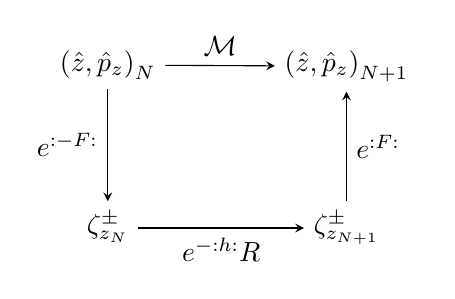
\begin{tikzpicture}
        \matrix (m) [matrix of math nodes,row sep=4em,column sep=4em,minimum width=2em]{
            \left(\hat{z}, \hat{p}_z\right)_N    &    \left(\hat{z}, \hat{p}_z\right)_{N+1} \\
            \zeta_{z_N}^{\pm}{}                  &    \zeta_{z_{N+1}}^{\pm}{}  \\
        };
        \path[-stealth]
        (m-1-1) edge node [above] {\( \mathcal{M} \)} (m-1-2)
        (m-1-1) edge node [left] {\( e^{:-F:} \)} (m-2-1)
        (m-2-1.east|-m-2-2) edge node [below] {\( e^{-:h:} R \)} (m-2-2)
        (m-2-2) edge node [right] {\( e^{:F:} \)} (m-1-2);
    \end{tikzpicture}
    \caption{Illustration of the coordinate transformations and change of the one-turn map. This diagram reads from Courant-Snyder coordinates at turn \(N\) in the top left, and shows both paths to reach the Courant-Snyder coordinates at turn \(N+1\) in the top right.}
    \label{figure:coordinate_transformations}
\end{figure}

\subsection{Spectral Contribution}
\label{subsec:spectral_contribution}

Each term in the summations of \cref{equation:linearly_normalized_coordinates_after_N_turns} corresponds to a certain mode in the beam motion and contributes to a specific frequency in the spectrum of the motion~\cite{PHD:Bengtsson}.
Said spectrum may be determined by a frequency analysis of the turn-by-turn beam position data, through means of a Fourier transform.
In this spectrum, an \gls{RDT} \(f_{jklm}\) at a specific location in the machine contributes to lines in the horizontal and vertical spectra according to~\cite{PHD:Bengtsson,PRAB:Franchi:Emittance_Sharing_Coupling}:

\begin{equation}
    \begin{aligned}
        H(1-j+k, m-l) &= 2 j \abs{f_{jklm}} \left( 2 I_x \right)^{\frac{j+k-1}{2}} \left( 2 I_y \right)^{\frac{l+m}{2}} \text{ ,}\\
        V(k-j, 1-l+m) &= 2 l \abs{f_{jklm}} \left( 2 I_x \right)^{\frac{j+k}{2}} \left( 2 I_y \right)^{\frac{l+m-1}{2}} \text{ ,}
    \end{aligned}
    \label{equation:rdt_contribution_to_spectrum_line}
\end{equation}
where in the parentheses multiples of the fractional tunes are given.
For example, \(H(0,1)\) indicates an observed line at \(1 \times Q_y\) in the horizontal spectrum.
% \Cref{figure:example_spectrum} shows an example of a spectrum from a measurement at the \gls{LHC}, where the main lines are highlighted.

In principle the \(\abs{f_{jklm}}\) may be determined by a comparison of the amplitude of various spectral lines.
In practice, some additional considerations need to be taken, as decoherence of a kicked beam can lead to a reduction in the amplitude of the spectral lines observed, or the fact that the contributions of different \glspl{RDT} might not be distinct.
More details are given in \cref{chapter:lhc_omc}.

\subsection{Amplitude Detuning}
\label{subsection:amplitude_detuning}

The \gls{ampdet} is the variation of the \gls{tune} with the single particle emittance.
It can be described with a Taylor expansion of the tune \(Q_z\) around the unperturbed tune \(Q_{z, 0}\) as:

\begin{equation}
    \begin{aligned}
    Q_z \left( \varepsilon_x, \varepsilon_y \right) & = Q_{z, 0} + \frac{\partial Q_z}{\partial \varepsilon_x} \varepsilon_x + \frac{\partial Q_z}{\partial \varepsilon_y} \varepsilon_y \\
                                                    & + \frac{1}{2!} \left(\frac{\partial^2 Q_z}{\partial \varepsilon_x^2} \varepsilon_x^2 + \frac{\partial^2 Q_z}{\partial \varepsilon_x \partial \varepsilon_y} \varepsilon_x \varepsilon_y + \frac{\partial^2 Q_z}{\partial \varepsilon_y^2} \varepsilon_y^2 \right) + \ldots \text{ ,}
    \end{aligned}
    \label{equation:tune_taylor_expansion}
\end{equation}
where \(\varepsilon_z = 2 J_z\) is the invariant of motion in the transverse plane \(z\).
The first order terms of the amplitude detuning, \(\frac{\partial Q_z}{\partial \varepsilon_x}\) and \(\frac{\partial Q_z}{\partial \varepsilon_y}\), are generated by octupoles and by the second order contribution of sextupoles~\cite{BOOK:Bazzani:Normal_Form_Approach_Betatron_Motion}; while the following terms come from higher order multipoles.
The amplitude detuning is a good indication of the machine non-linearities.

\section{Betatron Coupling}
\label{section:betatron_coupling}

When the betatronic motion of particles in transverse planes are independent of each other, they are said to be \concept{uncoupled}.
In particle colliders such as the \gls{LHC} this is the desired behaviour.
When these motions share a dependency, they are said to be \concept{coupled}, and one refers to this phenomenon as \gls{betatron_coupling}, or linear coupling.
The transverse motions of particles in an accelerator may couple due to a variety of factors, with solenoid and \gls{skew} quadrupole fields being the primary sources of linear coupling.

In the \gls{LHC} the main contribution to coupling comes from unwanted \gls{skew} quadrupolar fields.
These mostly arise from \gls{normal} quadrupoles mounted with a rotation error with respect to the longitudinal axis, but also from field imperfection from other magnets and feed-down from higher order magnets.
An example of a normal and skew quadrupole is given in \cref{figure:normal_vs_skew_quadrupole}.

\begin{figure}[!hbt]
    \centering
    \begin{subfigure}[b]{0.49\textwidth}
        \centering
        \includegraphics[width=\textwidth]{Figures/Beam_Dynamics_Theory/bfield_normal_multipole_order_2.pdf}
        \caption{Normal quadrupole.}
        \label{subfigure:normal_quadrupole}
    \end{subfigure}
    \hfill
    \begin{subfigure}[b]{0.49\textwidth}
        \centering
        \includegraphics[width=\textwidth]{Figures/Beam_Dynamics_Theory/bfield_skew_multipole_order_2.pdf}
        \caption{Skew quadrupole.}
        \label{subfigure:skew_quadrupole}
    \end{subfigure}
    \caption{Illustration of a \gls{normal} (left) and \gls{skew} (right) magnetic quadrupole and their magnetic field lines.}
    \label{figure:normal_vs_skew_quadrupole}
\end{figure}

\Gls{betatron_coupling} needs to be kept under control as it can perturb the tune feedback systems and push tunes into resonances, lead to a reduction in the dynamic aperture~\cite{PA:Ripken:Impact_Linear_Coupling_Nonlinear_Dynamics} or loss of beam stability~\cite{MASTERS:Soubelet:Optics_Octupole_PyHEADTAIL,PRAB:Carver:Transverse_Instabilities_With_Coupling}.

\subsection{Parametrization of Betatron Coupling}
\label{subsection:parametrization_of_betatron_coupling}

There are different ways to parametrize coupled motion in a particle accelerator, the two most common being the Edwards-Teng~\cite{IEEE:Edwards:Parametrization_Linear_Coupled_Motion} and Mais-Ripken~\cite{AIP:Willeke:Methods_Beam_Optics} parametrizations.
For coupled motion a dependency between the horizontal and vertical planes is introduced, and as mentioned in \cref{subsection:equations_of_motion_and_twiss_parameters} the transverse motions can no longer be described by two independent \(2 \times 2\) matrices.
Instead, it is described by a \(4 \times 4\) matrix \(\hat{\mathbf{M}}\) such that

\begin{equation}
    \hat{\mathbf{M}} = \begin{pmatrix}
        \mathbf{P} & \mathbf{p} \\
        \mathbf{q} & \mathbf{Q}
    \end{pmatrix} \text{ ,}
    \label{equation:coupled_motion_matrix}
\end{equation}
where \(\mathbf{P}\), \(\mathbf{p}\), \(\mathbf{q}\) and \(\mathbf{Q}\) are \(2 \times 2\) matrices.
In the absence of \gls{betatron_coupling}, it follows that \(\mathbf{p}\) and \(\mathbf{q}\) are \num{0}.
Magnetic elements introducing coupling between the horizontal and vertical planes have non-zero terms in the respective \(\mathbf{p}\) and \(\mathbf{q}\) of their transfer matrices.
For instance, the transfer matrix of a \gls{skew} quadrupole can be written

\begin{equation}
    \mathbf{M}_\mathrm{skew\ quad.} = \begin{pmatrix}
        \mathbf{M_x}    & \mathbf{M_{xy}}  \\
        \mathbf{M_{yx}} & \mathbf{M_y}   \\
    \end{pmatrix} \text{ ,}
    \label{equation:skew_quad_transfer_matrix}
\end{equation}
where, using \(\omega = \sqrt{k_{1s}} \ge 0\) for clarity, the various \(2 \times 2\) matrices are expressed as~\cite{Lecture:Wolski:Dynamical_Maps_Linear_Elements}:

\begin{equation}
    \begin{aligned}
        \mathbf{M_x} &= \begin{pmatrix}
            \frac{1}{2} \left( \cos \left(\omega L\right) + \cosh \left(\omega L\right)\right)        &  \frac{1}{2 \omega} \left( \sin \left(\omega L\right) + \sinh \left(\omega L\right)\right) \\
            -\frac{\omega}{2} \left( \sin \left(\omega L\right) - \sinh \left(\omega L\right)\right)  &  \frac{1}{2} \left( \cos \left(\omega L\right) + \cosh \left(\omega L\right) \right)
        \end{pmatrix} \text{ ,} \\
        \mathbf{M_{xy}} &= \begin{pmatrix}
            \frac{1}{2} \left( \cos \left(\omega L\right) - \cosh \left(\omega L\right)\right)        &  \frac{1}{2 \omega} \left( \sin \left(\omega L\right) - \sinh \left(\omega L\right)\right) \\
            -\frac{\omega}{2} \left( \sin \left(\omega L\right) + \sinh \left(\omega L\right)\right)  &  \frac{1}{2} \left( \cos \left(\omega L\right) - \cosh \left(\omega L\right)\right)
        \end{pmatrix} \text{ ,} \\
        \mathbf{M_{yx}} &= \begin{pmatrix}
            \frac{1}{2} \left( \cos \left(\omega L\right) - \cosh \left(\omega L\right)\right)              &  \frac{1}{2 \omega} \left( \sin \left(\omega L\right) - \sinh \left(\omega L\right)\right) \\
            -\frac{\omega}{2} \left( \sin \left(\omega L\right) + \sinh \left(\omega L\right)\right)  &  \frac{1}{2} \left( \cos \left(\omega L\right) - \cosh \left(\omega L\right)\right)
        \end{pmatrix} \text{ ,} \\
        \mathbf{M_y} &= \begin{pmatrix}
            \frac{1}{2} \left( \cos \left(\omega L\right) + \cosh \left(\omega L\right)\right)              &  \frac{1}{2 \omega} \left( \sin \left(\omega L\right) + \sinh \left(\omega L\right)\right) \\
            -\frac{\omega}{2} \left( \sin \left(\omega L\right) - \sinh \left(\omega L\right)\right)  &  \frac{1}{2} \left( \cos \left(\omega L\right) + \cosh \left(\omega L\right)\right)
        \end{pmatrix} \text{ .}
    \end{aligned}
    \label{equation:skew_quad_transfer_matrix_sub_matrices}
\end{equation}

\subsubsection*{Edwards-Teng Parametrization}

The effect of \gls{betatron_coupling} can, figuratively, be seen as a rotation of the beam ellipse.
In the Edwards-Teng parametrization presented in~\cite{IEEE:Edwards:Parametrization_Linear_Coupled_Motion}, the linear coupling is then described by a symplectic rotation \(\mathbf{R}\) of \(\hat{\mathbf{M}}\) into its normal modes form \(\overline{\mathbf{M}}\), as shown in \cref{equation:edwards_teng_parametrization}.
In this new frame the motion is decoupled, and all the information on the coupling is held by the matrix \(\mathbf{R}\).

\begin{equation}
    \overline{\mathbf{M}} = \left(
        \begin{array}{cc}
            \mathbf{X} & 0 \\
            0 & \mathbf{Y}
    \end{array} \right) = \mathbf{R} \hat{\mathbf{M}} \mathbf{R}^{-1} \text{ .}
    \label{equation:edwards_teng_parametrization}
\end{equation}

Edwards and Teng have characterized the transformation \(\mathbf{R}\) with the symplectic matrix:

\begin{equation}
    \mathbf{R} =\left(
        \begin{array}{cc}
            \mathbf{I} \cos \theta & -\mathbf{K}^{-1} \sin \theta \\
            \mathbf{K} \sin \theta & \mathbf{I} \cos \theta
    \end{array} \right) \text{ ,}
    \label{equation:edwards_teng_rotation_matrix}
\end{equation}
where \(\mathbf{I}\) is the \(2 \times 2\) unit matrix and \(\mathbf{K}\) is a \(2 \times 2\) symplectic matrix, such that \(det(\mathbf{K}) = 1\).
The coupled motion may then be described by the uncoupled \gls{Twiss_parameters} seen in \cref{subsection:equations_of_motion_and_twiss_parameters}, together with the elements of matrix \(\mathbf{K}\) and Teng's angle of rotation \(\theta\).
In the case that \(\theta = 0\), the matrix \(\mathbf{R}\) is the identity matrix and as a result it will not rotate any of the modes: this corresponds to uncoupled motion.

The Edwards-Teng parameterization is used in the \gls{MADX} code~\cite{CODE:MADX_guide} when handling coupled motion.
In \gls{MADX} the relevant parameters are \(\alpha_{x, y}\), \(\beta_{x, y}\), \(\mu_{x, y}\), \(\gamma_{x, y}\) and \(r_{11}\), \(r_{12}\), \(r_{21}\), \(r_{22}\), where \(r_{11} \ldots r_{22}\) correspond to the elements of \(\mathbf{K}\) multiplied by \(\tan(\theta)\).

\subsubsection*{Mais-Ripken Parametrization}

The approach of Mais and Ripken was developed in~\cite{REPORT:Ripken:AllGerman} and is more accessible in~\cite{AIP:Willeke:Methods_Beam_Optics, REPORT:Borchardt:Calculation_Beam_Envelopes}.
It defines so-called \concept{Ripken parameters} \(\alpha_{kj}\), \(\beta_{kj}\) and \(\gamma_{kj}\), where \(k = 1 \ldots 3\) refers to the plane (\(x, y, \ldots\)) and the index \(j\) refers to the eigenmodes, that are accurate in the presence of coupling.
In the coupled case, all \(\beta_N\) are non-zero and \(\beta_{11}, \beta_{22}\) are distinctively different from \(\beta_x, \beta_y\), respectively.
The relations linking these new parameters to the \gls{Twiss_parameters} can be found in~\cite{IOP:Lebedev:Betatron_Motion_Coupling}.
% The relations linking these new parameters to the Twiss parameters is~\cite{IOP:Lebedev:Betatron_Motion_Coupling}:

% \begin{equation}
%     \begin{aligned}
%     \beta_x &= \frac{\beta_{11}}{1-u} \text{ ,} \quad \alpha_x = \frac{\alpha_{11}}{1-u}, \\
%     \beta_y &= \frac{\beta_{21}}{1-u} \text{ ,} \quad \alpha_y = \frac{\alpha_{21}}{1-u},
%     \end{aligned}
%     \label{equation:ripken_to_twiss_parameters}
% \end{equation}
% where \(\sin \phi = \pm \sqrt{u}\) is the rotation of the x-y plane. When φ = 0 there is no coupling and β x = β 11
The Mais-Ripken parameterization is the basis of the \gls{PTC}~\cite{CODE:Schmidt_Forest:PTC}'s handling of coupled dynamics. 

\subsubsection*{Coupling and Beam Matrix}

Considering the \num{2}D case of a given transverse direction the so-called \concept{beam matrix} or \concept{sigma matrix}, which is the covariance matrix of the particle distribution, is expressed as:

\begin{equation}
    \sigma = \begin{pmatrix}
        \sigma_{11} & \sigma_{12} \\
        \sigma_{21} & \sigma_{22}
    \end{pmatrix} = \begin{pmatrix}
        \left\langle z^2 \right\rangle   & \left\langle z p_z \right\rangle   \\
        \left\langle p_z z \right\rangle & \left\langle p_{z}^2 \right\rangle
    \end{pmatrix}  \text{ .}
    \label{equation:2d_sigma_matrix}
\end{equation}
\vspace{1pt}

\noindent
where the brackets indicate an average over all particles in the beam.
Note that this matrix is symmetric with \(\sigma_{12} = \sigma_{21}\).

Considering that the \gls{Twiss_parameters} and the emittance defining the phase space ellipse are related to the various moments of the beam distribution as

\begin{equation}
    \begin{gathered}
        \epsilon_z = \sqrt{\left\langle z^2 \right\rangle \left\langle p_z^2 \right\rangle - \left\langle z p_z \right\rangle^2}  \text{ ,}  \\
        \beta_z    = \frac{\left\langle z^2 \right\rangle}{\epsilon_z}                                                            \text{ ,}  \\
        \alpha_z   = -\frac{\left\langle z p_z \right\rangle}{\epsilon_z}                                                         \text{ ,}  \\
        \gamma_z   = \frac{\left\langle p_z^2 \right\rangle}{\epsilon_z}                                                          \text{ ,}
    \end{gathered}
\end{equation}
one can relate them to the sigma matrix via the emittance through:

\begin{equation}
    \sigma = \varepsilon_z \begin{pmatrix}
        \beta_z & - \alpha_z \\
        - \alpha_z & \gamma_z
    \end{pmatrix}  \text{ .}
    \label{equation:2d_sigma_matrix_to_twiss_parameters}
\end{equation}
\vspace{1pt}

\noindent
When considering the full \num{4}D transverse space one can express the beam matrix \(\Sigma\) as a block diagonal \(4 \times 4\) matrix with the respective horizontal and vertical sigma matrices on the diagonal and zeros elsewhere.
In the presence of coupling, the general covariance matrix has non-zero terms outside its diagonal and takes the form of \cref{equation:4d_sigma_matrix}:

% See https://research.bangor.ac.uk/portal/files/28932262/untitled.pdf
\begin{equation}
    \Sigma = \begin{pmatrix} 
        \sigma_{11} & \sigma_{12} & \sigma_{13} & \sigma_{14} \\
        \sigma_{21} & \sigma_{22} & \sigma_{23} & \sigma_{24} \\
        \sigma_{31} & \sigma_{32} & \sigma_{33} & \sigma_{34} \\
        \sigma_{41} & \sigma_{42} & \sigma_{43} & \sigma_{44}
    \end{pmatrix} = \begin{pmatrix}
        \left\langle x^2 \right\rangle           &  \left\langle x p_x \right\rangle           &  \left\langle x y \right\rangle           &  \left\langle x p_y \right\rangle           \\
        \left\langle x p_x \right\rangle  &  \left\langle p_x^2 \right\rangle         &  \left\langle p_x y \right\rangle  &  \left\langle p_x p_y \right\rangle  \\
        \left\langle x y \right\rangle           &  \left\langle p_x y \right\rangle           &  \left\langle y^2 \right\rangle           &  \left\langle y p_y \right\rangle           \\
        \left\langle x p_y \right\rangle  &  \left\langle p_x p_y \right\rangle  &  \left\langle y p_y \right\rangle  &  \left\langle p_y^2 \right\rangle
    \end{pmatrix} \text{ .}
    \label{equation:4d_sigma_matrix}
\end{equation}
\vspace{1pt}

Through \(\Sigma\) the coupling can be characterized by the values of the cross-planes elements \(\left\langle x y \right\rangle\), \(\left\langle x p_y \right\rangle\), \(\left\langle p_x y \right\rangle\) and \(\left\langle p_x p_y \right\rangle\).
Through the symmetry (for instance, \(\left\langle x y \right\rangle = \left\langle y x \right\rangle\)) only those four terms are needed.

The angle of rotation \(\theta\) in the Edwards-Teng parametrization is related to these terms through~\cite{EPAC:Cai:Luminosity_of_Asymmetric_e+e-_Collider_with_Coupling_Lattices}:

% See: https://ados.web.psi.ch/opa/inside.pdf Eq. (37)
\begin{equation}
    \tan{2 \theta} = \frac{2 \Sigma_{xy}}{\Sigma_{xx} - \Sigma_{yy}} = \frac{2 \sigma_{13}}{\sigma_{11} \sigma_{33}} \text{ .}
    \label{equation:edwards_teng_theta_to_sigma_matrix_terms}
\end{equation}

In the Mais-Ripken parameterization, the Ripken parameters are constructed in order to be related to the \(\Sigma\) matrix in a similar way than shown in \cref{equation:2d_sigma_matrix_to_twiss_parameters} for the \num{2}D uncoupled case.

\subsection{Coupled Motion}
\label{subsection:coupled_motion}

In the first order, according to \cref{equation:resonance_condition}, linear coupling drives the two resonances \(Q_x + Q_y = p\) and \(Q_x - Q_y = p\), with \(p \in \mathcal{Z}\).
These are respectively called the \concept{sum and difference resonances}, and in their vicinity the beam dynamics are heavily influenced.
% To higher order \gls{betatron_coupling} may also give stationary terms in the Hamiltonian (a tune shift), driving the \(2 Q_x\) and \(2 Q_y\) resonances, but these effects are typically negligible.

The impact of linear coupling on the beam motion has been studied through Hamiltonian perturbation theory~\cite{PHREV:Guignard:Betatron_Coupling_Radiation,BOOK:Wiedemann:Particle_Accelerator_Physics}, and through the normal form and \gls{RDT} formalism~\cite{PHD:Franchi}.
As the transverse tunes approach the difference resonance, the emittance is described by:

\begin{equation}
    \varepsilon_x + \varepsilon_y = \mathrm{const} \text{ ,}
    \label{equation:coupled_emittances_difference_resonance}
\end{equation}
and as the resonance is approached the beam motion may not become unstable.
Instead, there is a periodic exchange of emittance between the transverse planes, which leads to a beating in the betatron oscillation amplitudes.

The relation between the \concept{unperturbed tunes} \((Q_x, Q_y)\) and the \concept{coupled tunes} \((Q_1, Q_2)\) is given by~\cite{CAS:Bryant:Theory_Weak_Betatron_Coupling}:

\begin{equation}
    \begin{aligned}
        Q_1 &= Q_x- \frac{\Delta}{2} + \frac{\sqrt{\Delta^2 + \abs{C^{-}}}}{2} \text{ ,} \\
        Q_2 &= Q_y+ \frac{\Delta}{2} - \frac{\sqrt{\Delta^2 + \abs{C^{-}}}}{2} \text{ ,}
    \end{aligned}
    \label{equation:unperturbed_tunes_to_coupled_tunes}
\end{equation}
with \(\Delta\) being the unperturbed fractional tune split and \glssymbol{Cminus} the linear coupling coefficient, a parameter describing the strength of the coupling.

When \(\Delta \gg \abs{C^{-}}\), away from the resonance, the observed oscillations modes \((Q_1, Q_2)\) are almost identical to the uncoupled tunes \((Q_x, Q_y)\).
When the tunes are moved closer together, approching the difference resonance (\(\Delta \rightarrow 0\)), the perturbed tunes are forced apart by the coupling and a minimal tune separation \(\Delta Q_{\mathrm{min}}\) can be observed.
The \glssymbol{Cminus} of \cref{equation:unperturbed_tunes_to_coupled_tunes}, named the \gls{Cminus}, corresponds this separation.
\Cref{figure:closest_tune_approach} shows an illustration of the phenomenon in the vicinity of the resonance, where both the unperturbed (dashed) and coupled (colored) fractional tunes are plotted against the uncoupled tune split.

\begin{figure}[!htb]
    \centering
    \includegraphics[width=0.9\linewidth]{Figures/Beam_Dynamics_Theory/closest_tune_approach_schematic.pdf}
    \caption{Illustration of coupled and uncoupled fractional tunes versus the uncoupled tune split. Courtesy of J. Keintzel~\cite{PHD:Keintzel}.}
    \label{figure:closest_tune_approach}
\end{figure}

On the other hand, when approaching the sum resonance the emittances follow:

\begin{equation}
    \varepsilon_x - \varepsilon_y = \mathrm{const} \text{ .}
    \label{equation:coupled_emittances_sum_resonance}
\end{equation}

This resonance allows for unstable motion as only the difference in emittance is constrained.
Therefore, it is common to choose a working point far from the sum resonance.
In the \gls{LHC}, the working points (visible on \cref{figure:tune_diagram_fifth_order}) are set such that the linear coupling is dominated by the difference resonance: the fractional tunes are \((Q_x, Q_y) = (0.28 \text{,} 0.31)\) at injection and \((Q_x, Q_y) = (0.31 \text{,} 0.32)\) for squeezed beams and collisions\footnote{The LHC working point is actually more diverse and will be discussed in more details in the next chapter.}.

\subsection{Linear Coupling Resonance Driving Terms}
\label{subsection:measurement_coupling_rdts}

Linear coupling in the \gls{LHC} is dominated by the contribution of \gls{skew} quadrupole fields, which lead to terms \(\propto xy\) in the Hamiltonian.
According to the resonance relation of \cref{equation:resonance_condition} and as seen in \cref{subsection:coupled_motion}, this gives rise to the \glspl{RDT} \(f_{1001}\) and \(f_{0110}\), which correspond to the \(Q_x - Q_y = p\) difference resonance; and \(f_{1010}\) which corresponds to the \(Q_x + Q_y = p\) sum resonance.

The \(f_{1001}\) and \(f_{0110}\) describe the same dynamics but the former is for the horizontal plane while the latter is for the vertical plane.
Since they describe the same dynamics it is custom to label both of them as \(f_{1001}\), which is a convention used throughout this document.

It was mentioned in \cref{subsection:coupled_motion} that the \gls{LHC} working point is selected to be close to the stable difference resonance, and as a consequence in the LHC the \(\abs{f_{1001}}\) dominates relative to the \(\abs{f_{1010}}\).
These \glspl{RDT} can be expressed as a function of the uncoupled lattice parameters at the location of both the coupling-contributing elements and the observation point \(s\) as~\cite{PHREV:Guignard:Betatron_Coupling_Radiation}:

\begin{equation}
    \begin{aligned}
        f_{1001}(s) &= - \frac{1}{4 \left(1 - e^{2 \pi i \left(Q_x - Q_y \right)}\right)} \sum_l k_l \sqrt{\beta_x^l \beta_y^l} e^{i \left(\Delta \phi_x^{s l} - \Delta \phi_y^{s l}\right)} \text{ ,} \\
        f_{1010}(s) &= - \frac{1}{4 \left(1 - e^{2 \pi i \left(Q_x + Q_y \right)}\right)} \sum_l k_l \sqrt{\beta_x^l \beta_y^l} e^{i \left(\Delta \phi_x^{s l} + \Delta \phi_y^{s l}\right)} \text{ ,}
    \end{aligned}
    \label{equation:coupling_rdts_from_skew_quads}
\end{equation}
where \(k_l\) is the \(l\)th integrated \gls{skew} quadrupole strength, \(\beta_{x,y}^{l}\) are the \glspl{beta-function} at the location of the \(l\)th skew quadrupole, \(Q_{x,y}\) are the horizontal and vertical tunes, and \(\Delta \phi_{x,y}^{s l}\) are the phase advances from the \(l\)th skew quadrupole to the observation point at the longitudinal coordinate \(s\).
The summation is done over all contributing \gls{skew} quadrupoles.

These \glspl{RDT} can be related to the strength of the coupling \(\Delta Q_{\mathrm{min}}\), and as such the \glssymbol{Cminus} can be expressed in relation to the \(f_{1001}\) \gls{RDT}.
In~\cite{PHD:Franchi} a simple version of this relation was established as:

\begin{equation}
    \abs{C^{-}} \approx 4 \Delta \frac{1}{N} \sum_{i=1}^N \abs{f_{1001}}_i \text{ ,}
    \label{equation:deltaqmin_from_f1001_franchi}
\end{equation}
where the summation is done over the \(N\) observation points, and \(\Delta\) is the fractional tune split.
A more accurate relation was established in~\cite{PRAB:Persson:Improved_Control_Betatron_Coupling}, which is:

\begin{equation}
    \abs{C^{-}} = \abs{\frac{4 \Delta}{2 \pi R} \oint d s f_{1001} e^{-i \left(\phi_x - \phi_y \right) + i s \Delta / R} } \text{ ,}
    \label{equation:deltaqmin_from_f1001}
\end{equation}
where the dependence of variables on the position \(s\) was omitted for clarity.

In~\cite{PHREV:Guignard:Betatron_Coupling_Radiation} the equations of motion are solved perturbatively under the influence of a weak \gls{skew} quadrupole strength \(j(s)\).
Assuming that the machine is close to the difference coupling resonance, \(\Delta = Q_x - Q_y \rightarrow 0\), the \glssymbol{Cminus} can be approximated as:

\begin{equation}
    \abs{C^{-}} = \frac{1}{2 \pi} \abs{ \oint ds \sqrt{\beta_x(s) \beta_y(s)} j(s) e^{-i \left( \phi_x - \phi_y \right) + i \frac{s \Delta}{R}} } \text{ ,}
    \label{equation:deltaqmin_guignard}
\end{equation}
where \(s\) is the position around the ring, \(\beta_{x,y}\) are the horizontal and vertical \(\beta\)-functions, \(\phi_{x,y}\) are the phase advances and \(R\) is the radius of the machine.

\section{Luminosity}
\label{section:luminosity}

The \gls{LHC} machine being a particle collider, it is operated to produce collisions between two counter-rotating beams and to produce data for \gls{HEP} \glspl{experiment}.
As the studied interactions coming from these collisions are rare, a substantial volume of statistics is required. 
Naturally, the performance of the machine is then described by the number of collisions provided to experiments as well as the center-of-mass energy of these collisions.

As a figure of merit for the number of collisions the \gls{luminosity} is used.
The \concept{instantaneous luminosity} \(\mathcal{L}\) is the proportional factor between the number of events per unit of time \(dR / dt\) and the process cross-section \(\sigma_{\mathrm{cross}}\):

\begin{equation}
    \dfrac{dR}{dt} = \mathcal{L} \sigma_{\mathrm{cross}} \text{ .}
    \label{equation:instantaneous_luminosity_definition}
\end{equation}

The instantaneous luminosity is given in units of inverse barns per second (\unit{\per\barn\per\second}), where \(\left[ b \right] = \) \qty{1e-24}{\square\centi\meter}.
For a collider with Gaussian beams, it can be expressed as~\cite{CERN:Herr:Concept_Luminosity}:

\begin{equation}
    \mathcal{L} = \frac{f_{\mathrm{rev}} N_1 N_2}{4 \pi \sigma_x \sigma_y} S \text{ ,}
    \label{equation:luminosity_gaussian_beams}
\end{equation}
where \(f_{\mathrm{rev}}\) is the revolution frequency of particle bunches, \(N_1\) and \(N_2\) are the number of particles in each beam, and \(\sigma_{x,y}\) are the transverse beam sizes at the interaction points.
\(S\) is the \concept{luminosity reduction factor} and depends on various parameters such as crossing angles, orbit offsets, beam-beam interactions, beam tilts in the case of \gls{flat_optics} etc.
For Gaussian bunches colliding with a \concept{crossing angle} \(\theta\), where \(\sigma_s \gg \sigma_{x,y}\) and neglecting other contributions, the luminosity reduction factor is approximated by~\cite{CERN:Herr:Concept_Luminosity}:

\begin{equation}
    S \approx \frac{1}{\sqrt{1 + \left( \frac{\theta}{2} \frac{\sigma_s}{\sigma_x} \right)^2}} \text{ .}
    \label{equation:luminosity_reduction_factor}
\end{equation}
\\
The luminosity can be influenced by the local presence of \gls{betatron_coupling} through its impact on beam size, as will be discussed in \cref{chapter:ir_local_coupling}.
As seen in \cref{equation:gaussian_beam_transverse_beam_size} the beam sizes directly depend on the \(\beta\)-function at the \gls{IP}, \glssymbol{betastar}, which then defines the collider's performance from the point of view of the optics.
Indeed, the smaller the \(\beta^{\ast}\) the smaller the beam sizes, and the more collisions will be produced per bunch crossing.

The \concept{integrated luminosity}, the accumulated luminosity over a given period of time, is given by:

\begin{equation}
    \mathcal{L}_{\mathrm{int}} = \int_{t_1}^{t_2} \mathcal{L} \mathrm{d}t \text{ .}
    \label{equation:integrated_luminosity}
\end{equation}

The integrated luminosity is usually in units of \unit{\per\femto\barn} \(=\) \qty{1e39}{\per\square\centi\meter}.
The total number of collisions, or events, over said time period is then:

\begin{equation}
    \mathrm{N_{events}} = \mathcal{L}_{\mathrm{int}} \sigma_{\mathrm{cross}} \text{ .}
    \label{equation:total_number_collisions}
\end{equation}

Throughout luminosity production, the instantaneous luminosity naturally decreases as more and more particles are lost to collisions~\cite{PRES:Hostettler:LHC_Lumi_Lifetime}.
Any particle losses happening before colliding the beams will lead to a reduction of the initial \(N_{1,2}\) and of the resulting integrated luminosity of the given fill.\\

\Gls{luminosity} production requires a good control of the linear optics, both for the quality of the optics themselves but also for a smooth and safe operation.
Many non-linear contributions may also influence the dynamics away from the linear regime, leading to a deterioration of the dynamics and, down the line, the luminosity.
Therefore for a particle collider like the \gls{LHC} a good control of all effects influencing the beam dynamics is required, and methods to both measure and correct any deviations from the ideal machine are a necessity.
An overview of these is given in \cref{chapter:lhc_omc}.

\glsresetall                                     % reset glossary entries counts for the next chapter

\chapter{Optics Measurements and Corrections at the LHC}
\label{Chapter:LHC_OMC} % For referencing the chapter elsewhere, use \cref{Chapter:LHC_OMC}

The Large Hadron Collider (LHC) is a \qty{26.659}{\kilo\metre} synchrotron collider located at the European Center for Nuclear Research (CERN), on the French-Swiss border.
It is part of CERN's Accelerator Complex, illustrated in \cref{figure:cern_accelerator_complex}, a chain of particle accelerators progressively bringing protons and heavy ions up to an energy of \qty{6.8}{\tera\electronvolt} per beam, as of \num{2023}.

\begin{figure}[!htb]
  \centering
  \includegraphics*[width=0.9\linewidth]{Figures/Optics_Measurements_Corrections_at_LHC/cern_accelerator_complex.png}
  \caption{The CERN Accelerator Complex in \num{2022}, not to scale~\cite{Website:CERN_Accelerator_Complex_Resource}. For typical LHC operation, a proton beam is produced in \(\mathrm{LINAC}\)~\num{4} and follows the chain: \(\mathrm{LINAC}\)\num{4} \(\rightarrow\) \(\mathrm{PSB}\) \(\rightarrow\) \(\mathrm{PS}\) \(\rightarrow\) \(\mathrm{SPS}\) \(\rightarrow\) \(\mathrm{LHC}\).}
  \label{figure:cern_accelerator_complex}
\end{figure}

Accelerated particles go through a chain of different particle accelerators before reaching their experimental destinations.
For protons colliding in the LHC, the first step is a linear accelerator, LINAC\num{4}, which accelerates them up to a kinetic energy of \qty{160}{\mega\electronvolt}.
Next, the protons are injected into the Proton Synchrotron Booster (PSB), where they are accelerated to an energy of \qty{1.4}{\giga\electronvolt}.
The next stage is the Proton Synchrotron, in which they will reach \qty{25}{\giga\electronvolt}; then the Super Proton Synchrotron (SPS) where they are accelerated to \qty{450}{\giga\electronvolt}, when they are finally injected into the LHC.

The LHC circulates two counter-rotating hadron beams, each in their ring, which are made to collide at four Interaction Points (IPs) to provide data for High Energy Physics (HEP) experiments.
The main data-taking experiments on the LHC are ATLAS~\cite{Website:ATLAS,Website:ATLAS_CDS}, LHCf~\cite{Website:LHCf,Website:LHCf_CDS}, ALICE~\cite{Website:ALICE,Website:ALICE_CDS}, CMS~\cite{Website:CMS,Website:CMS_CDS}, TOTEM~\cite{Website:TOTEM,Website:TOTEM_CDS}, LHCb~\cite{Website:LHCb,Website:LHCb_CDS} and MoEDAL~\cite{Website:MOEDAL,Website:MOEDAL_CDS}.
The LHC is currently the world's highest-energy hadron colliding machine, colliding beams at \qty{13.6}{\tera\electronvolt} center-of-mass energy as of Run~\num{3}, \num{2023}.

%----------------------------------------------------------------------------------------

\section{The LHC Lattice}
\label{section:lhc_lattice}

The LHC lattice consists of eight \intro{octants} each intersected by an \intro{Insertion Region} (IR).
Conventionally, the segment between two \IRs is called an \intro{arc} and the arc between IR1 and IR2 is named Arc12, and similarly for other arcs.
An octant is defined as going from mid-arc to mid-arc around a given \IR which is located at its center.
Each octant is named according to the \IR at its center: the octant with \(\mathrm{IR1}\) at its center is named Octant1, and similarly for other octants.
An illustration and a detailed description on naming conventions can be found in \cref{appendix:naming_conventions}.
% The \IRs host either an \intro{Interaction Point} (IP) where beams are made to collide (ATLAS at IP1, ALICE at IP2, CMS at IP5 and LHCb at IP8) or important instrumentation (momentum cleaning at IR3, Radio-Frequency cavities at IR4, beam dump system at IR6 and betatron cleaning at IR7).

Beam~1 rotates clockwise in its ring when viewing the LHC from above, and Beam~2 rotates counter-clockwise as viewed from above.
The beams occupy separate apertures, or beam pipes, except in the \IRs where they are eventually made to collide.
The layout of the LHC can be seen in \cref{figure:lhc_layout}, and full details can be found in the LHC Design Report~\cite{BOOK:Bruning:LHC_Design_Report_Main_Ring,BOOK:Bruning:LHC_Design_Report_Infrastructure,BOOK:Benedikt:LHC_Design_Report_Injector_Chain}.

\begin{figure}[!htb]
  \centering
  \includegraphics*[width=0.8\linewidth]{Figures/Optics_Measurements_Corrections_at_LHC/temp_lhc_schematic_layout.png}
  \caption{Schematic of the LHC layout, adapted from~\cite{JOI:Aaboud:Comparison_Simulated_Observed_Beam_Background_ATLAS}. \todo{Or get and adapt Axel code.}}
  \label{figure:lhc_layout}
\end{figure}

\subsection{The LHC Arcs}
\label{subsection:lhc_arcs}

\begin{figure}[!hbt]
  \centering
  \includegraphics*[width=0.9\linewidth]{Figures/Optics_Measurements_Corrections_at_LHC/lhc_fodo_cell.pdf}
  \caption{\todo{Caption lhc fodo cell.}}
  \label{figure:lhc_fodo_cell}
\end{figure}

\begin{figure}[!hbt]
  \centering
  \includegraphics*[width=0.9\linewidth]{Figures/Optics_Measurements_Corrections_at_LHC/lhc_arc23.pdf}
  \caption{\todo{Caption lhc arc23.}}
  \label{figure:lhc_arc23}
\end{figure}

\subsection{The LHC Experimental Interaction Regions (EIR)}
\label{subsection:lhc_eirs}

An insertion region in which beams are made to collide is called an \intro{Interaction Region}, or sometimes experimental interaction region.

\todo{Mention for figure that the matching section marked in the plot includes the dispersion suppressor.}

\begin{figure}[!hbt]
  \centering
  \includegraphics*[width=0.9\linewidth]{Figures/Optics_Measurements_Corrections_at_LHC/ir5_surroundings_optics_2.pdf}
  \caption{The horizontal and vertical \betafunctions in the LHC around IP5 at injection optics (top) and collision optics (bottom). Notice the drastically different scales on the vertical axes.}
  \label{figure:ir5_and_around}
\end{figure}

\subsection{Interaction Points}
\label{subsection:interaction_points}

\subsection{The LHC Triplet}
\label{subsection:lhc_triplet}

\subsection{Separation Dipoles}
\label{subsection:separation_dipoles}

\subsection{Matching Section}
\label{subsection:matching_section}

\subsection{Dispersion Suppressor}
\label{subsection:dispersion_suppressor}

\begin{figure}[!hbt]
  \centering
  \includegraphics*[width=0.9\linewidth]{Figures/Optics_Measurements_Corrections_at_LHC/lhc_dispersion_suppressor.pdf}
  \caption{\todo{Caption lhc dispersion suppressor.}}
  \label{figure:lhc_dispersion_suppressor}
\end{figure}

%----------------------------------------------------------------------------------------

\section{The Operational Cycle of the LHC}
\label{section:lhc_operational_cycle}

The LHC operational cycle~\cite{Report:LHCModes}, shown in \cref{figure:lhc_cycle}, starts with a pre-cycle of certain magnetic elements~\cite{Report:LHCMagnetsPreCycles}.
During pre-cycle no beams are present in the rings and the respective element currents are increased up to several \qty{}{\tera\electronvolt}, to ensure the reproducibility of the magnetic fields over successive fills.
After the pre-cycle, beams are injected from the Super Proton Synchrotron (SPS) at an energy of \qty{450}{\giga\electronvolt}.
At injection optics the \(\beta^{\ast}_{x,y}\) is \qty{11}{\metre}.
The number of bunches, their intensity and their filling pattern~\cite{Report:LHCStandardFillingSchemes} depends strongly on the experimental demands.
For optics measurements a single low intensity bunch of about \num{e10} particles is used for each beam.
After injection, the beam energy is increased up to collision energy (\qty{6.8}{\tera\electronvolt} in Run~3) while the \(\beta^{\ast}\) is squeezed.
This process, called combined ramp and squeeze has been used in the LHC since 2017~\cite{IPAC:Camillocci:CombinedRampAndSqueeze}.
Before then the squeezing process only started once the energy had reached collision value.
At top energy with squeezed optics, also called as flat-top, the optics is confirmed and eventually adjusted before collisions start with stable beams.
The fill ends when dumping the beams, after which the cycle ends by a ramp down of the magnets' currents.

\begin{figure}[h]
    \centering
    \includegraphics*[width=0.9\linewidth]{Figures/Optics_Measurements_Corrections_at_LHC/lhc_cycle.pdf}
    \caption{Illustration of the LHC operational cycle.}
    \label{figure:lhc_cycle}
\end{figure}

Starting in Run~\num{3}, some additional complexities were added to the cycle that are not shown in \cref{figure:lhc_cycle}.
In \num{2022} a \betastar-leveling was introduced, were collisions start at a higher \(\beta^{\ast}\) than \qty{30}{\centi\meter}, and the \(\beta^{\ast}\) is progressively reduced to \qty{30}{\centi\meter} in order to limit pile-up for the experiments.
\todo{REF.}
In \num{2023}
\todo{REF.}

%----------------------------------------------------------------------------------------

\section{Optics Measurements and Corrections}
\label{section:optics_measurements_and_corrections}

The LHC requires good control of the optics functions, and for instance a good control of the \betafunctions is essential for safe beam operations due to the destructive power of the LHC beams.
Moreover, a good control of the \(\beta^{\ast}\) is necessary to guarantee good luminosity production.
To validate the machine optics and to identify possible errors beam measurements are performed, from which corrections bringing the machine as close to the nominal scenario as possible are calculated and applied. 
This chapter gives an overview of the LHC machine and its operational cycle, as well as the essential beam instrumentation used for optics measurements.
Additionally, concepts of corrections methods are given.

\subsection{Beam Instrumentation for Optics Measurements}

\subsubsection{Beam Position Monitors}

% \subsubsection{Beam Current Monitors}

\subsubsection{BBQ System for Tune Measurements}

\subsubsection{Excitation Devices}


Measurements of beam optics are done by generating large transverse beam oscillations, typically much larger than the natural beam size.
A non-destructive method for beam excitation in hadron machines is achieved using an AC-dipole

\subsection{Optics Measurements}
\label{subsection:optics_measurements}

- excite
- harmonic analysis
- optics analysis

\subsubsection{Turn-by-turn Measurements}

\subsection{Correction Principles}

\subsubsection{Global Corrections}

\subsubsection{Local Corrections}

Here mention the need for new stuff as things get hairy with the LHC upgrades.
% \chapter{Interaction Region Local Coupling Correction in the LHC} % Main chapter title
\label{chapter:IR_Local_Coupling} % For referencing the chapter elsewhere, use \cref{chapter:IR_Local_Coupling}

\todo{Some paragraph before the first section.}

%----------------------------------------------------------------------------------------

\section{Local Betatron Coupling in the Interaction Regions}

\textbf{List of things to include in this section:}
\begin{itemize}
    \item Refer to previous chapter plots of IR for the very large \(\beta\)-functions in the triplet quadrupoles, tilts in these magnets have the potential to drastically contribute to the magnitude of the \(f_{1001}\) term, and therefore to the coupling in the interaction region and, if not compensated properly, to the coupling in the whole machine
    \item Equivalency of Ripken and Tracking when looking at beam size (or later?)
    \item Projection of the beam size growth and lumi in the LHC vs HL-LHC
    \item Include the parts in the "relevant theory" section of my PRAB paper
    \item ALICE \num{2018} ion run lumi issue
\end{itemize}

\begin{equation}
    \langle z \rangle = \sqrt{\varepsilon_1 \beta_{1z} + \varepsilon_2 \beta_{2z}}, \quad z \in\{x, y\} ,
    \label{equation:lebedev_beam_size}
\end{equation}
where \(\varepsilon_1\) and \(\varepsilon_2\) are the horizontal and vertical emittances, respectively.
\Cref{figure:ip_ellipses_from_coupling} shows a reconstruction of transverse beam sizes at IP\num{5} under varying strength of a local coupling bump.
While the beam ellipses show a \(\gg\) \qty{99}{\percent} overlap indicating a negligible tilt effect, the beam size in the most affected case is about \qty{250}{\percent} of the uncoupled case.

\begin{figure}[!htb]
    \centering
    \includegraphics*[width=0.99\columnwidth]{Figures/IR_Coupling_Correction/triplet_tilts_to_rdts.pdf}
    \caption{\todo{The Cminus here was \num{3.84e-2}.}}
    \label{figure:triplet_tilts_to_rdts}
\end{figure}

\begin{figure}[!htb]
    \centering
    \includegraphics*[width=0.75\columnwidth]{Figures/IR_Coupling_Correction/ellipses_various_coupling_bumps.pdf}
    \caption{Transverse beam sizes at IP\num{5} at \qty{6.8}{\tera\electronvolt} and \(\beta^{\ast}=\)~\qty{30}{\centi\meter} with normalized emittances \(\varepsilon_x = \varepsilon_y =\)~\qty{3.75}{\micro\meter} and for different strengths of a local coupling bump around the IP. The ellipses are reconstructed through the \(\sigma_{11}\), \(\sigma_{13}\) and \(\sigma_{33}\) terms of the sigma matrix, obtained from MAD-X.}
    \label{figure:ip_ellipses_from_coupling}
\end{figure}

Instantaneous luminosities calculated for~\cref{figure:lhc_vs_hllhc_beam_size_and_lumi_growths}, in the absence of crossing angles, are done so according to~\cite{CERN:Herr:Concept_Luminosity}:

\begin{equation}
    \mathcal{L} = \frac{N_1 N_2 f_{rev} N_b}{2 \pi \sqrt{\left( \sigma_{x, 1}^2 + \sigma_{x, 2}^2 \right)} \sqrt{\left( \sigma_{y, 1}^2 + \sigma_{y, 2}^2 \right)}} ,
    \label{equation:luminosity_double_beams}
\end{equation}
where \(N_{n}\) is the number of protons per bunch in beam \(n\), \(f_{rev}\) the revolution frequency of particles, \(N_b\) the number of bunches per beam and \(\sigma_{z, n}\) is the size at the IP of beam \(n\) in the transverse plane \(z\), calculated according to \cref{equation:lebedev_beam_size}.

\begin{figure}[!htb]
    \centering
    \includegraphics*[width=0.99\columnwidth]{Figures/IR_Coupling_Correction/lhc_vs_hllhc_combined.pdf}
    \caption{Relative values of the RMS beam size at IP\num{1} (\textcolor{mplblue}{blue}) as well as luminosity (\textcolor{mplorange}{orange}) for different strengths of a local coupling bump around the IP made with skew quadrupoles, for the LHC (filled) and HL-LHC V1.5 (dashed). Beam sizes are calculated according to \cref{equation:lebedev_beam_size} and luminosities according to \cref{equation:luminosity_double_beams}. In the case of the HL-LHC, the relative beam size increase and subsequent luminosity loss are greater due to the larger \(\beta\)-functions in the triplet.}
    \label{fig:lhc_vs_hllhc_beam_size_and_lumi_growths}
\end{figure}

\section{Current Correction Methods and Their Limitations}

Overview of IR Difficulties (phase advances suck, DFFT of x -jpx, no instruments, SbS errors)

In the LHC, a skew quadrupole corrector is installed on each side of colliding IPs, just before the third triplet quadrupole \(\mathrm{Q3}\) on the side of the IP.
Due to their location, these correctors are single aperture magnets meaning that both beams are passing through a single cavity, and feel the same magnetic field.
As the triplet quadrupoles - also single aperture magnets - are expected to be most of the contribution to local coupling, the local error to be corrected should be the same for both beams and such an arrangement of correctors is manageable.

Say that looking at RDTs is just not straightforward, and give example with plot below. Can you guess who's better? I forgot already.
\begin{figure}
    \centering
    \includegraphics*[width=0.99\linewidth]{Figures/IR_Coupling_Correction/similar_rdts_different_ip1_lumi.pdf}
    \caption{Similarly looking coupling RDTs from two measurements (top and bottom) in the LHC \num{2022} commissioning. One scenario leads to a \qty{20}{\percent} luminosity decrease at IP\num{1} compared to the other. Can you tell which is which?}
    \label{figure:guess_rdts}
\end{figure}

\begin{table}[!hbt]
    \centering
    \begin{tblr}{colspec={ccccc}}
        \hline
        \textbf{Magnet} & \textbf{K\(_{1S}\) [m\(^{-2}\)]}    \\
        \hline
        MQSX.3R[IP] \(\rightarrow K_{1S}\)  &  \num{1E-4}   \\
        MQSX.3L[IP] \(\rightarrow K_{1S}\)  &  \num{-1E-4}  \\
        \hline
    \end{tblr}
    \caption{Definition of one unit of the colinearity knob, a powering setting of the IR skew quadrupole correctors.}
    \label{table:colin_knob}
\end{table}

\begin{figure}
    \centering
    \includegraphics[width=0.9\linewidth]{Figures/IR_Coupling_Correction/corrector_package.png}
    \caption{Layout of the triplet magnets and the linear and nonlinear correctors in the LHC experimental insertions~\cite{CERN:Bruning:Dynap_Studies}, showing common aperture magnets. The Q\num{1}, Q\num{2}a/b and Q\num{3} are triplet quadrupoles while the C\num{0}, C\num{1}, C\num{2} and C\num{3} are corrector packages with the field order indicated below. D\num{1} is the separation dipole, diverging Beam \num{1} and Beam \num{2} to their respective beam lines. The skew quadrupole correctors correspond to order a\num{2} and are located in the C\num{2} package.}
    \label{figure:lhc_corrector_layout}
\end{figure}

\todo{Here include also the stuff that didn't work (CRDTs, k-modulation, etc.)}

\section{Rigid Waist Shift for Local Coupling Correction}

\subsection{Concept and Simulations}

\begin{figure}
    \centering
    \includegraphics[width=0.9\textwidth]{Figures/IR_Coupling_Correction/rigid_waist_shift_effect_combined.pdf}
    \caption{Simulated effect of the designed rigid waist shift knob on the \(\beta^{\ast} =\) \qty{30}{\centi\metre} collision optics. The \textcolor{mplblue}{blue} line represents the waist displacement from the design location and is almost completely linear with the knob setting. The \textcolor{mplorange}{orange} and \textcolor{mplgreen}{green} lines represent the horizontal and vertical \(\beta\)-functions change at the IP point itself as the waist is displaced, respectively. The minima of the parabolas are not found at the zero knob setting as the design optics include a very small waist.}
    \label{figure:rigid_waist_shift_knob_effect1}
\end{figure}

\begin{figure}[!htb]
    \centering
    \includegraphics*[width=\columnwidth]{Figures/IR_Coupling_Correction/waist_shift_leaks_rdts.pdf}
    \caption{Linear coupling RDTs in the vicinity of IP\num{1} under a coupling bump, with (\textcolor{mplr}{red}) and without (\textcolor{mplb}{blue}) an RWS. The vertical \textcolor{mqsx_green}{green} lines represent the positions of the skew quadrupoles correctors (MQSX.\num{3}[RL]\num{1}) used to implement the coupling bump. A colinearity knob setting of \num{10} and a rigidity waist shift knob setting of \num{1} were used, which results in a \qty{0.5}{\percent} change in the triplet powering knob and a \qty{43.5}{\centi\meter} shift of the beam waists.}
    \label{figure:rdt_leak}
\end{figure}

\begin{figure}[!htb]
    \centering
    \includegraphics*[width=0.99\columnwidth]{Figures/IR_Coupling_Correction/colin_knob_vs_waist_shift.pdf}
    \caption{Impact of the colinearity knob on the global \(\abs{C^{-}}\), calculated according to \cref{equation:deltaqmin_from_f1001}, with and without applying an RWS.}
    \label{figure:knob_to_cminus_with_waist}
\end{figure}

\Cref{figure:cminus_colin_vs_tilt_with_waist} shows the values of the resulting \(\abs{C^{-}}\) across the parameter space when an RWS is applied.

\begin{figure}[!htb]
    \centering
    \includegraphics*[width=0.99\columnwidth]{Figures/IR_Coupling_Correction/cminus_colin_tilt_compensation_with_waist.pdf}
    \caption{Resulting \(\abs{C^{-}}\) (\cref{equation:deltaqmin_from_f1001}) for various combinations of tilt error and colinearity knob settings, when applying an RWS.}
    \label{figure:cminus_colin_vs_tilt_with_waist}
\end{figure}

\Cref{figure:beam_size_colin_vs_tilt_no_waist} shows the resulting beam size increase as a ratio to the nominal beam size across the same parameter space, highlighting that minimization of the growth is possible though a wrong setting would enhance the phenomenon.

\begin{figure}[!htb]
    \centering
    \includegraphics*[width=0.99\columnwidth]{Figures/IR_Coupling_Correction/ip_beam_size_growth_colin_tilt_compensation_no_waist.pdf}
    \caption{Resulting beam size (\cref{equation:lebedev_beam_size}) increase for identical settings of tilt error and colinearity knob settings as \cref{figure:cminus_colin_vs_tilt_with_waist}, but without an RWS.}
    \label{figure:beam_size_colin_vs_tilt_no_waist}
\end{figure}

\subsection{Determining Corrections}

Blah.

\subsubsection*{Rigid Waist Shift Procedure}

Bleh.

%----------------------------------------------------------------------------------------

\section{Experimental Results from the LHC \num{2022} Commissioning}

Can refer to appendix \Cref{appendix:experimental_knobs} for the fills used.

\begin{table}[!htb]
    \centering
    \caption{Luminosity gains observed at the main experiments ATLAS and CMS from the method's suggested corrections.}
    \begin{tblr}{colspec={ccc}}
        \hline
        \SetCell[r=2,c=1]{m,c} \textbf{Experiment} & \SetCell[c=2]{c} \textbf{Luminosity Gain [\unit{\percent}]}                     \\
        \cline{2,3}                                &    \(\beta^{\ast} = \) \qty{30}{cm}    &    \(\beta^{\ast} = \) \qty{42}{cm}    \\
        \hline
        \textbf{ATLAS (IP\num{1})}                 &    \num{9.7}                           &     \num{5.2}                          \\
        \textbf{CMS (IP\num{5})}                   &    \num{3.5}                           &     \num{1.5}                          \\
        \hline
    \end{tblr}
    \label{table:rws_lumi_gains}
\end{table}

\section{Operation with Limited Correctors Availability}

Mitigation Options in Case of MQSX Failures
\todo{Uncomment text when I get here, take mostly the structure of the IPAC23 article and project update V. Go deeper in details (see commented out subsections).}

% \subsection{Lifetime Considerations of MQSX Elements}

% Explain that there is a real risk that some of our MQSX magnets die, especially the ones in IR1 (ATLAS).
% In this case, we will need a containment plan, as not only are they used for the but the local corrections they are a part of are a baseline for us to compute higher order terms corrections.

% \Cref{table:correctors_peak_dose} reproduced from slide 23~\cite{Evian21:Cerutti:TripletLifetime}:

% \begin{table}[!htb]
%     \centering
%     \caption{Expected total received dose of the corrector magnets located in the triplets for the main IRs. Table reproduced from~\cite{Evian21:Cerutti:TripletLifetime}. The entries marked with \asterisk assume an IR\num{1} polarity inversion in the middle of \num{2025}.}
%     \begin{tblr}{colspec={ccc}}
%         \hline
%         \SetCell[r=3,c=1]{m,c} \textbf{Magnets}             &  \SetCell[c=2]{c} \textbf{Peak Dose [\unit{\mega\gray}]}                                                                                     \\
%         \cline{2,3}                                         &  With ATLAS Variable (Fixed) Angle                        &    +\num{2025} (as \num{2023}/\num{2024})                                        \\
%         \cline{2,3}                                         &  After \qty{395}{\femto\barn^{-1}}                        &    After \qty{480}{\femto\barn^{-1}}                                             \\
%         \hline
%         \textcolor{red}{\textbf{MCBX\num{1} (IR\num{1})}}   &    \textcolor{red}{\num{8.5} (\num{8.5})}                 &     \textcolor{red}{\num{11} (\num{11}) $/$ \asterisk \num{10.5} (\num{10.5})}   \\
%         \textcolor{red}{\textbf{MCBX\num{1} (IR\num{5})}}   &    \num{6}                                                &     \textcolor{red}{\num{7.5}}                                                   \\
%         \textbf{MCBX\num{2} (IR\num{1})}                    &    \num{3.5} (\num{3.5})                                  &     \num{4} (\num{4}) $/$ \asterisk \num{4} (\num{4})                            \\
%         \textbf{MCBX\num{2} (IR\num{5})}                    &    \num{2}                                                &     \num{2.5}                                                                    \\
%         \textcolor{red}{\textbf{MQSX (IR\num{1})}}          &    \textcolor{red}{\num{7.5} (\num{7.5})}                 &     \textcolor{red}{\num{9} (\num{9}) $/$ \asterisk \num{9} (\num{9})}           \\
%         \textcolor{red}{\textbf{MQSX (IR\num{5})}}          &    \textcolor{red}{\num{8} (\num{8})}                     &     \textcolor{red}{\num{9.5} (\num{9.5})}                                       \\
%         \textbf{MCBX\num{3} (IR\num{1})}                    &    \num{5} (\num{5})                                      &     \num{6} (\num{6.5}) $/$ \asterisk \num{6} (\num{6})                          \\
%         \textbf{MCBX\num{3} (IR\num{5})}                    &    \num{3}                                                &     \num{3.5}                                                                    \\
%         \hline
%     \end{tblr}
%     \label{table:correctors_peak_dose}
% \end{table}

% \todo{Important quote from the end of the presentation:}
% "Assuming a limit of \qty{6}{\mega\gray} for the corrector magnets in the triplet, this is expected to be reached in the four \(\mathrm{MCBX.1}\) and four \MQSX by the end of \num{2024}."

% This means in simple terms that MQSX dying will drastically impact the LHC's operations, and potentially shut the machine down.

% \subsection{Tilt of Triplet Elements}

% Talk about what we want to do (tilt Q3 or Q2) to induce a skew component + simulation results.
% Found settings of the Q3 or Q2 that would negate the MQSX one determined in beam test / commissioning.
% Show some plots, and come up with the tilt values that would be needed to do the compensation.

% Also show we have a very minimal beta-beating from this.
% Show we have had a look at different optics (30cm and 1m betastar) and it works for both.

% \subsubsection*{Operational Constraints}

% The LHC systems are not meant for this, but for vertical alignment of these magnets!
% System relies on bellows: 2 pieds IP side and 1 pied other side for Q2 for instance.
% This means that inducing rotation is not only not the design purpose, but also imperfect (on move les 2 pieds pour essayer de mimer une rotation mais c'est pas parfait).
% Would be very good to have a plot of the assemblies here to show what I mean. Ask MP people? See in the LHC design report?

% It is considered by MP people to be quite dangerous to do this unless forced to (read an MQSX dies), especially in cold mass, as if we damage the belows then we're in for 1 year of shutdown to repair it.
% Say that for these reasons we decided not to test this concept in the machine, unfortunately.

% Could show plots here (see "Living with Local Coupling" section of my project update V) about the effect on luminosity: what reduction are we looking at 

% \subsection{Warm Skew Quadrupole Replacement}

% Here talk about how there is space between D1 and TAN for a magnet, and we could put a warm skew quadrupole there.
% Show some schematic.
% Show some calculations of how the gradient should be, how long the element should be etc.

% It has considerations such as being imbalanced (asymmetric) with the remaining MQSX, limiting the available aperture etc.

% \subsection{Feed-Down from High Order Correctors}

% Mention here that we consider using sextupolar and octupolar (MCSSX and MCSX) magnets to generate feed-down to coupling.
% However, these elements are not strong enough to generate the same effect that the MQSX do, so this is not really an option.

% \subsection{Adapting the Optics Squeezing Scheme}

% We could change things in the squeeze to compensate for the absence of an MQSX.
% Potentially squeeze harder on one IP (the one with a missing element).
% Potentially squeeze similarly for both but when the unaffected IP stops the squeeze, the other one keeps going to lower \betastar, and the lost luminosity at beginning of fill is made up for starting this moment.
% Not cool because LHCb prefers long fill + impact on BBLR?

% Plot to show the ratio of luminosity as in PowerPoint?

% \subsection{Potential MDs / Exp. Results}

% Talk about how this could be tested.
% If we do get MD blocks for this in September, include the data here.

% %----------------------------------------------------------------------------------------

\section{Conclusions}

%----------------------------------------------------------------------------------------
% \chapter{Machine Learning for Interaction Region Local Coupling}
\label{chapter:ml_local_coupling}

Machine learning methods have found their application in a variety of fields including technology development, scientific research, medical diagnosis and business insights.
The now widespread application of machine learning techniques demonstrates their applicability to various challenges and tasks.

In recent years machine learning has been successfully applied to various areas of accelerator physics~\cite{PRAB:Edelen:Machine_Learning_Optimization_Particle_Accelerator_Systems,PRAB:Gao:Bayesian_Optimization_Trajectory_Alignment,PRAB:Ivanov:Physics_Based_Deep_Neural_Networks_Beam_Dynamics,PRL:Roussel:Phase_Space_Reconstruction_Neural_Networks,PRAB:Kranjcevic:Multiobjective_Optimization_Dynamic_Aperture,PRL:Jalas:Bayesian_Optimization_Laser_Plasma_Accelerator,PRL:Duris:Bayesian_Optimization_Free_Electron_Laser,IPAC:Biedron:Adding_Data_Science_and_More_Intelligence_to_Our_Accelerator_Toolbox,IEEE:Edelen:Neural_Networks_Modeling_Control_Particle_Accelerators,PRAB:Emma:Machine_Learning_Longitudinal_Phase_Space_Prediction,IBIC:Xu:Machine_Learning_Image_Processing_Technology_Application_in_Bunch_Longitudinal_Phase_Data_Information_Extraction}, including at the \gls{LHC}~\cite{PRAB:Fol:Detection_Faulty_BPMs,EPJP:Fol:Supervised_Learning_Reconstruction_Magnet_Errors,PHD:Fol:Application_ML_Beam_Optics}.
The primary purpose of the work presented hereafter is to explore the possibility of applying machine learning techniques to the subject of local \gls{IR} coupling in the LHC.

%----------------------------------------------------------------------------------------

\section{Relevant Concepts of Machine Learning}
\label{section:concepts_of_machine_learning}

Machine learning can be seen as the intersection of statistics and computer science.
The key characteristics of machine learning are described by T. Mitchell as~\cite{BOOK:Mitchell:Machine_Learning}:

\begin{quoteblock}
    Machine learning techniques aim to build computer programs and algorithms that automatically improve with experience by learning from examples with respect to some class of task and performance measure, without being explicitly programmed.
\end{quoteblock}

A key characteristic distinguishing machine learning from conventional programming is the program's ability to automatically achieve performance improvements based on provided data.
This section provides a quick introduction to relevant paradigms and concepts of machine learning, primarily derived from~\cite{BOOK:Mitchell:Machine_Learning,BOOK:Hastie:Elements_Statistical_Learning} where one can find detailed discussions on the subject.
The focus is kept only on particular concepts relevant to the work presented in this chapter.

\subsection{Defining a Machine Learning Task}

In the context of machine learning, \concept{learning} refers to the process of improving performance.
Generally speaking a model can improve its performance by adjusting its parameters with respect to provided data, in order to refine the approximation function that is derived from said data. 
It is important to note that a trained model will always remain an approximation of the relationship in the underlying data, but with a good enough training this approximation should be sufficiently reliable for the specific task at hand.
The requirements on the model's performance in terms of accuracy, precision and reliability depend on a particular task and application domain.

The chosen performance criteria, the type of experience to be gained through learning and the specific approach and algorithm are specific to the task that must be learned.
These three parameters - task, measure of performance and source of experience - are the fundamentals of a well-defined machine learning problem.
In practice, it is reflected in the selection of appropriate learning method and function approximation algorithm, definition of the loss function and its acceptable values, as well as the preparation of data.
The latter can be non-trivial and require dedicated techniques and algorithms.

\subsection{Supervised and Unsupervised Learning}

Two main approaches are available in machine learning depending on the problem definition and the availability and structure of the learning examples.

\concept{Unsupervised learning} is characterized by the use of unlabeled datasets.
Unsupervised learning algorithms solve tasks where only input data is available, and are used to analyze and cluster inputs by discovering patterns in data without the need for human intervention, hence them being \textit{unsupervised}.
They are suitable for tasks such as anomaly detection, signal denoising, dimensionality reduction, and feature extraction.
% They are used for tasks such as clustering, association and dimensionality reduction.
% Clustering groups unlabeled data based on their similarities or differences, association finds relationships between variables in a given dataset and dimensionality reduction reduces the number of data inputs to a manageable size while also preserving the data integrity.

\concept{Supervised learning} is characterized by the use of labeled datasets.
These datasets are used to train - or supervise - the model to learn how to accurately classify data or predict outcomes.
During the training, predictions are computed from the inputs and compared to the known corresponding outputs.
By adjusting the parameters of the model - or approximation function - the quantified difference between computed predictions and correct outputs, the so-called \concept{loss function}, is minimized.
% Providing known labeled inputs and outputs allows the model to measure its accuracy and adjust its parameters during learning.
Supervised learning is typically used for \concept{classification} and \concept{regression} tasks.
Classification tasks aim to accurately assign test data into specific categories, and regression tasks aim to understand and approximate the relationship between dependent and independent variables in order to predict the outcome of a given input.

\subsection{Regression Models}

In the case of regression problems, the regression function is what is being approximated by the model.
The core model principles are outlined below.

\subsubsection*{Linear Models}

Linear models compute the estimates of the output values using a linear function of the input variables~\cite{PNAS:Lai:Strong_Consistency_Least_Squares_Estimates_Regression_Models}.
For regression tasks, the estimation for the predicted output \(\hat{y}\) of a linear model is expressed as:

\begin{equation}
    \hat{y} = w_0 + \sum_{i=1}^{N} w_i x_i \text{ ,}
    \label{equation:linear_regression_prediction}
\end{equation}
where \(\vec{x}\) is the input vector containing \(N\) features, and \(\vec{w}\) is the vector containing the learned coefficients of the model, with \(w_0\) being the bias.
In a simple case (see \cref{figure:ml_underfitting_overfitting} below) \(\hat{y}\) is a scalar, but it is usually a vector of dimension \(K\).
In this case the model parameters \(w\) are then represented as an \(N \times K\) matrix.

Typically, linear regression models are trained using the \concept{least squares} method, which minimizes the residual sum of squared errors between the predicted and actual output values.
Given a set of \(N\) samples from the training dataset, and \(y\) being the true output for a given sample, the linear model's parameters are updated during training with each incoming sample, minimizing:

\begin{equation}
    RSS(\hat{w}) = \sum_{m=1}^{N} (y_m - \hat{y}_m)^2 \text{ .}
    \label{equation:least_squares_rss}
\end{equation}

After training, the resulting coefficients should be sufficiently general to generate accurate predictions for all provided data samples.

\subsubsection*{Polynomial Regression}

Some learning tasks, due to the complex properties of the data, require non-linear predictors.
For instance, this is the case when fitting a one dimensional polynomial function of degree \(n\):

\begin{equation}
    p(x) = a_0 + a_1 x + a_2 x^2 + \dots + a_n x^n \text{ ,}
    \label{equation:polynomial_function}
\end{equation}
\vspace{1pt}

\noindent
where \((a_0, \ldots, a_n)\) is a vector of coefficients of size \(n+1\).
One way to train a model to approximate such a function is to reduce the problem to linear regression~\cite{BOOK:ShalevShwartz:Understanding_Machine_Learning}.
To do so one can introduce a mapping such that \(\psi(x)=\left(1, x, x^2, \ldots, x^n\right)\), which reduces the problem to:

\begin{equation}
    p(\psi(x)) = a_0 + a_1 x + a_2 x^2 + \ldots + a_n x^n = \langle \vec{a}, \psi(x) \rangle \text{ ,}
    \label{equation:polynomial_function_linear_mapping}
\end{equation}
\vspace{1pt}

\noindent
and the optimal vector \(\vec{a}\) can be found by minimizing the residual sum of squares (RSS) as in \cref{equation:least_squares_rss}.

\subsection{Generalization, Underfitting and Overfitting}
\label{subsection:generalization_underfitting_overfitting}

In supervised learning, one tries to train a model capable of making correct predictions on new, unseen data based on the experience and tuning acquired on the training data's known outputs.
This ability to predict on new data is called \concept{generalization}, and is the most important aspect of the built model~\cite{PR:Rosenblatt:Perceptron,BOOK:Bishop:Neural_Networks_Pattern_Recognition}.
A separate and unrelated test dataset is usually used in order to evaluate the predictive power of the model.
Most of the time, training and test datasets share enough similarities - properties and relations in the underlying data - such that the model can accurately predict on the test set.

However, in the case of highly complex models high accuracy can be achieved on the training data with poor prediction performance on the test data.
When too complex, models can tend to fit very closely to individual data points in the training data and extrapolate unexisting relations that will later on perform badly on new data.
This phenomenon is called \concept{overfitting}.
Similarly, when too simple for the data at hand the model will not be able to capture the underlying relations and will not be able to perform accurate predictions even on training data.
This is referred to as \concept{underfitting}.

\Cref{figure:ml_underfitting_overfitting} illustrates these concepts by showing an underfitting model, a model that generalizes well, and an overfitting model.
Though simple, this example highlights the importance of building a model that generalizes well.

\begin{figure}[!htb]
    \centering
    \includegraphics*[width=\textwidth]{Figures/ML_for_IR_Coupling/ml_underfitting_overfitting.pdf}
    \caption{Three examples showcasing models approximating (\textcolor{mplblue}{blue}) a true function (\textcolor{mplorange}{orange}) after training on provided samples (\textcolor{mplb}{dark blue}). Of the three models one is too simple and underfits (left), one generalizes properly (middle), and one is too complex and overfits (right). This plot was reproduced from the \textit{scikit-learn} documentation~\cite{CODE:scikit-learn, Website:ScikitLearn:Overfitting_Example}.}
    \label{figure:ml_underfitting_overfitting}
\end{figure}

One of the common ways to identify underfitting or overfitting is to provide validation data to the model in addition to the training data.
The training set is then used to drive the learning procedure, and after training the error is evaluated on the validation set.
When done properly, the model's performance on both training and validation sets should be nearly equal.
If the performance on the training set is substantially higher, the model has been overfitted and further adjustments on the model complexity are then required.

\subsubsection*{Regularized Regression}

A potential approach to avoid overfitting is to apply regularization during the model training by imposing a penalty on the update of the model's parameters.
As the model parameters are updated to attempt to fit every incoming input-output pair, the penalty constrains the change of these parameters such that the model becomes more robust against variations in the data.
This technique is known as \textit{L2 regularization}, and in the context of supervised regression \concept{ridge regression}~\cite{MIT:Rifkin:Regularized_Least_Squares}.

A ridge regressor minimizes the residual sum of squares introduced above by introducing a tuning parameter \(\alpha\) which mitigates the potential linear dependencies between different input variables in the dataset.
In the presence of such dependencies, parameters might be updated inappropriately during training in response to small changes in the model or the data.
The regression task is formulated as:
\begin{equation}
    \min _w \left|\left| w \vec{x} - \vec{y} \right|\right|_2^2 + \alpha \left|\left| w \right|\right|_2^2 \text{ ,}
    \label{equation:ridge_regression_regularization}
\end{equation}
where \(w\) is the matrix containing the parameters of the model, \(\vec{x}\) is the input data vector and \(\vec{y}\) the vector of targets to be predicted by the model.
With higher values of \(\alpha\) the changes in model parameters are reduced at each update step, helping to not overreact to correlated changes in the data.

It is also possible to mitigate overfitting by decreasing the number of input features while retaining only uncorrelated features for function approximation by the model.
\concept{Lasso regression}~\cite{JRSS:Tibshirani:Regression_Shrinkage_Selection_Via_Lasso} uses an \(L1\) norm to drive some regression coefficients to \(0\), which improves the model in terms of variance and allows for automatic feature selection.

To tune additional model parameters such as the ridge penalty \(\alpha\) or the number of input features to be retained in Lasso regression one can use \concept{cross-validation}, a resampling method which consists in randomly dividing the dataset into equally sized parts.
For instance, the dataset is divided in ten subsets and the model is fitted on nine of those while the loss is computed on the remaining subset.
This procedure is repeated for each of the ten subsets to be used for loss computation, and all ten estimates of the prediction error are averaged.
As the practice is part of the training process cross-validation is only applied to the training dataset, and the test dataset is still used only to evaluate a trained model's performance on unobserved data.

\section{Identification of Local Coupling Sources}

In the previous chapter, the negative impact of local \gls{IR} linear coupling in the \gls{LHC} has been extensively discussed, as well as the necessity of its identification and mitigation.
The precise knowledge of a coupling source's location and relative strength would be a valuable asset for further correction.
However, it was illustrated in \cref{section:current_correction_methods_and_their_limitations} how simply looking at patterns and jumps in the coupling \glspl{RDT} was not always sufficient to accurately pinpoint the  location of a source, nor can it be used in locations with little instrumentation or unfavorable conditions.
As machine learning techniques have found their application in a wide range of particle accelerator control tasks in the past~\cite{IPAC:Fol:Machine_Learning_Methods_for_Optics_Measurements_and_Corrections_at_LHC, IEEE:Edelen:Neural_Networks_Modeling_Control_Particle_Accelerators, EPAC:Bozoki:Neural_Networks_Orbit_Control_Accelerators, IPAC:Meier:Orbit_Correction_Studies_using_Neural_Networks, EPAC:Kijima:Beam_Diagnostic_System_for_Accelerator_using_Neural_Networks, PRAB:Fol:Detection_Faulty_BPMs, EPJP:Fol:Supervised_Learning_Reconstruction_Magnet_Errors}, the possibility of applying machine learning techniques to the detection of local IR coupling sources in the LHC was explored.

In order to perform a prediction of betatron coupling sources' locations, one first needs to compute the \(f_{1001}\) and \(f_{1010}\) coupling RDTs which will serve as input data for the model.
The strength and variations of the coupling RDTs throughout the machine is then used to estimate the location of coupling sources and their relative strengths.

In terms of machine learning, this task can be defined as a regression problem that can be solved by training a model using measurements and corresponding solutions.
Such a regression model requires a large dataset in order to be able to generalize and produce reliable results.
As in the real machine the true location of coupling sources is unknown, no real-world data is available for the training of machine learning models.

\subsection{Dataset Generation}

In order to create a training dataset simulations were performed with the \acrshort{MAD}-X~\cite{CODE:MADX_guide} code, in which random rotations around the \(s\)-axis are introduced into individually powered IR quadrupoles, in each IR.
The tilt generates a \gls{skew} quadrupolar component at the affected element and thus turns it into a source of coupling.
It has to be noted though, that in simulations only quadrupole tilts - given by the \(\mathrm{DPSI}\) variable in MAD-X - were used to generate coupling sources, which means other potential sources such as feed-down from higher order magnets were ignored in this study.

When generating the data from simulations, the introduced tilt components form the training output and the produced coupling RDTs generated from the perturbed optics functions are the input in the training dataset.
The data was generated for both Beam 1 and 2 using the \(\beta^{\ast}=\)~\qty{30}{\centi\meter} optics.
\Cref{figure:ml_local_sources_rdts} shows the reconstructed coupling RDTs for a given simulation in which a truncated Gaussian distribution of tilts was assigned to all independently powered IR quadrupoles Q\num{1} to Q\num{11} in IRs \numlist{1;2;5;8}.

\begin{figure}[!htb]
    \centering
    \includegraphics*[width=0.99\textwidth]{Figures/ML_for_IR_Coupling/ml_local_sources_rdts_combined.pdf}
    \caption{Beam~\num{1} (top) and Beam~\num{2} (bottom) coupling RDTs \(f_{1001}\) (\textcolor{mplblue}{blue}) and \(f_{1010}\) (\textcolor{mplorange}{orange}) after the implementation of tilt errors in the independently powered IR quadrupoles Q\num{1} to Q\num{11} in IRs \numlist{1;2;5;8}, for the \qty{6.8}{\tera\electronvolt} and \(\beta^{\ast}=\)~\qty{30}{\centi\meter} optics.}
    \label{figure:ml_local_sources_rdts}
\end{figure}

The standard deviation of the applied tilt errors Gaussian distribution was aligned with expected values from the element alignment precision in the LHC, after discussions with the alignment group.
Each sample of the dataset is obtained by applying the following steps in simulations:
\begin{enumerate}
    \item A truncated Gaussian distribution of tilt errors (\(\mathrm{DPSI}\)) is applied to quadrupoles Q\num{1} to Q\num{11} in IRs \numlist{1;2;5;8} for Beam~\num{1}.
    \item Quadrupoles located outside the IRs are excluded as these sources can be identified and compensated by other means.
    \item The coupling RDTs \(f_{1001}\) and \(f_{1010}\) are calculated at each \acrshort{BPM} from \gls{Twiss_parameters} for Beam~\num{1}.
    \item The \(\mathrm{DPSI}\) values for triplets are exported and applied to Beam 2, as these are common magnets and should share the error.
    \item A truncated Gaussian distribution similar to the one of step \num{1} is applied to the remaining quadrupoles Q\num{4} to Q\num{11} in IRs \numlist{1;2;5;8} for Beam~\num{2}.
    \item Coupling RDTs for Beam~\num{2} are calculated at each BPM as done for Beam~\num{1}.
    \item The real and imaginary parts of the coupling RDTs at each BPM and for each beam are concatenated in order to obtain a single vector of values for a given sample.
\end{enumerate}

To train the model the relation is flipped, and the introduced tilt errors have to be found based on given coupling RDTs computed from the perturbed optics.
Therefore, the coupling RDTs reconstructed at each BPM are considered as model input and a vector containing the predicted \(\mathrm{DPSI}\) value attributed to each affected quadrupole is the desired output.
\Cref{figure:ml_supervised_training_schematic} shows a conceptual schematic of the dataset generation and supervised model training process for this given application.
% More specifically,each block is repeated many times: the former during dataset generation and the latter for supervised training.

\begin{figure}[!htb]
    \centering
    \includegraphics*[width=0.99\textwidth]{Figures/ML_for_IR_Coupling/supervised_training_schematic.pdf}
    \caption{Conceptual representation of the dataset generation and supervised model training. This diagram is heavily inspired from~\cite{PHD:Fol:Application_ML_Beam_Optics}.}
    \label{figure:ml_supervised_training_schematic}
\end{figure}

A dataset of \num{50000} samples (each an individual simulation following the steps above) was divided into train and test sets (\qty{75}{\percent} and \qty{25}{\percent} respectively).
Each sample pair consists in \num{4424} inputs - real and imaginary parts of each coupling RDT for each BPM for each beam - and \num{160} outputs: one \(\mathrm{DPSI}\) value at each affected IR quadrupole.

In addition, in order to reproduce the uncertainty of the RDTs reconstructed from measurements, both train and test datasets were augmented by adding Gaussian noise to the RDTs.
The standard deviation of the added noise was determined by a statistical analysis of several measurements from the LHC Run~\num{2}.
\Cref{figure:rdts_stdev_batch} shows the standard deviation of measured coupling RDTs across Beam~\num{1} BPMs for a batch of measurements taken on April~\num{3}, \num{2018}.

\begin{figure}[!htb]
    \centering
    \includegraphics*[width=0.95\textwidth]{Figures/ML_for_IR_Coupling/ml_rdts_batch_stdev.pdf}
    \caption{Standard deviation of the coupling RDTs at BPMs for Beam~\num{1}, from a batch of measurements taken on April~\num{3}, \num{2018}. These data points were later divided into IR and arc BPMs to determine applied noise levels.}
    \label{figure:rdts_stdev_batch}
\end{figure}

After analyzing several such batches, the following noise levels to be added were determined:
\begin{itemize}
  \item Coupling RDTs at arc BPMs were noised with a truncated Gaussian distribution of standard deviation ranging from \num{0} to \num{1E-5} absolute error.
  \item Inner BPMs located in the IRs (number \num{1} to \num{6} from the IP) were noised with a truncated Gaussian distribution of standard deviation ranging from \num{0} to \num{1E-2} absolute error.
\end{itemize}

A new dataset was created for each combination of the noise levels mentioned above.
For instance, a given set had IR BPMs noised with a standard deviation of \num{1E-3} and arc BPMs with \num{1E-6}.
Similarly, several such datasets were created for different standard deviation of the introduced tilt errors.

\subsection{Model Training and Evaluation}

In this study models have been evaluated based on their \(R^2\) scores (coefficient of determination) as well as the normalized mean absolute error between the true output values and the model predictions.
Several models suited for regression tasks were tested, that are listed below, and a minimal amount of hyperparameter tuning was performed.

Each model was trained and evaluated on the various datasets generated, in order to assess their performance and usability in various realistic contexts of noise in the data. 
A simple least squares linear regression~\cite{PNAS:Lai:Strong_Consistency_Least_Squares_Estimates_Regression_Models} showed very good results on clean data, however its performance dropped drastically when applied to the noised datasets, down to unusable accuracy.
A decision tree regressor~\cite{BOOK:Breiman:Classification_Regression_Trees} and a random forest regressor~\cite{ML:Breiman:Random_Forests} showed poor performance on all datasets.
A ridge regressor model (see \cref{subsection:generalization_underfitting_overfitting}) showcased good performance on both clean and relatively low-noise datasets.

\Cref{figure:ridge_performance} shows the test performance of the ridge regressor~\cite{MIT:Rifkin:Regularized_Least_Squares} on noised datasets depending on the level of noise added to different BPMs, where the impact of noise on the reconstructed coupling RDTs is apparent.
In the top plot the Mean Absolute Error (MAE) - the sum of absolute errors divided by the sample size - was normalized to the standard deviation of the applied magnet tilts, \(\sigma_{\mathrm{DPSI}} =\)~\qty{1E-4}{\radian}.
In this figure each curve represents a noise level applied to arc BPMs data while each point on these curves corresponds to a noise level applied to the inner BPMs.
While dense, this representation allows to see the performance of the model on a wide range of noised datasets, for a single given distribution of the tilt errors.

\begin{figure}[!htb]
    \centering
    \includegraphics*[width=0.95\textwidth]{Figures/ML_for_IR_Coupling/ml_ridge_performance.pdf}
    \caption{Normalized mean absolute error (top) and \(R^2\) scores (bottom) of a ridge regressor on various datasets corresponding to different noise levels added to the coupling RDTs. The \(\sigma\) values indicated correspond to the standard deviation of the Gaussian noise distributions added to the coupling RDTs data.}
    \label{figure:ridge_performance}
\end{figure}

To the left of the plot at data points corresponding to low noise levels in IR BPMs, where for two of the curves (\textcolor{mplblue}{blue} and \textcolor{mplorange}{orange}) the model's performance is excellent.
Moving up one order of magnitude in the arc BPMs noise level (\textcolor{mplgreen}{green}) leads to a significant performance drop.
Point to the right of the plot, corresponding to increasing noise in IR BPMs data, also showcase a drop in performance down to an unusable model, with \(R^2 = 0.54\) in the worst case.

\Cref{figure:ridge_histograms} shows histograms of the distributions of true attributed errors, of the ridge regressor's predictions and of deviations to the true values.
These were obtained by evaluating the model on a noised dataset with \(\sigma_{\mathrm{DPSI}} =\)~\qty{1E-4}{\radian}, \(\sigma_{\mathrm{IRs}} = 10^{-5}\) and \(\sigma_{\mathrm{arcs}} = 10^{-6}\) (corresponding to the third leftmost point on the \textcolor{mplorange}{orange} curve in \cref{figure:ridge_performance}).
One can notice the histogram of deviations much more narrowly centered on \num{0} than that of the attributed errors, which is the sign of good performance.

\begin{figure}[!htb]
    \centering
    \includegraphics*[width=0.7\textwidth]{Figures/ML_for_IR_Coupling/ridge_histograms.pdf}
    \caption{Histograms of the true applied \(\mathrm{DPSI}\) values (\textcolor{ridgepurple}{purple}), the values predicted by the Ridge model (\textcolor{ridgeblue}{blue}) and the deviations from the predictions to the true values (\textcolor{ridgesalmon}{pink}) for a noised sample in the test dataset (\(\sigma_{\mathrm{DPSI}} =\)~\qty{1E-4}{\radian} and \(\sigma_{\mathrm{Arcs, IRs}} = 10^{-5}\)).}
    \label{figure:ridge_histograms}
\end{figure}

\Cref{figure:ridge_predictions} shows the ridge model's predictions on a sample from the same noised test dataset (\(\sigma_{\mathrm{DPSI}} =\)~\qty{1E-4}{\radian}, \(\sigma_{\mathrm{IRs}} = 10^{-5}\) and \(\sigma_{\mathrm{arcs}} = 10^{-6}\)), where a good agreement between the predicted and the assigned true values can be observed.
Prediction performance significantly degrades with the addition of noise, with sometimes predictions being off by an order of magnitude or more in the worst cases.

\begin{figure}[!htb]
    \centering
    \includegraphics*[width=0.95\textwidth]{Figures/ML_for_IR_Coupling/ml_ridge_regression_sample_predictions.pdf}
    \caption{True assigned (\textcolor{mplblue}{blue}) and predicted (\textcolor{mplorange}{orange}) \(\mathrm{DPSI}\) values with a ridge model for a given test dataset sample. Here the magnet names have been switched for numbers in order to improve clarity.}
    \label{figure:ridge_predictions}
\end{figure}

Results showing the best \(R^{2}\) scores obtained by each model on both clean and noised datasets are presented in \cref{table:ml_models_comparison}, where the ridge regressor clearly outperforms its counterparts.

\begin{table}[!hbt]
    \centering
    \begin{tblr}{colspec={ccc}}
        \hline
        \textbf{Model}             &   Clean Data     &   Noised Data     \\
        \hline
        Ridge Regressor            &   \num{0.9911}   &   \num{0.8934}    \\
        Linear Regression          &   \num{0.9913}   &   \num{0.5638}    \\
        Decision Tree Regressor    &   \num{0.1385}   &   \num{-0.0018}   \\
        Random Forest Regressor    &   \num{0.0175}   &   \num{-0.0009}   \\
        \hline
    \end{tblr}
    \caption{Comparison of the \(R^2\) score averaged over \num{1000} samples taken from the test dataset for different models. For the results in this table, the standard deviations of the applied noise were \(\sigma = 10^{-4}\) for IR BPMs and  \(\sigma = 10^{-6}\) for arc BPMs. The distribution of tilt errors had a standard deviation of \(\sigma =\)~\qty{1E-4}{\radian}.}
    \label{table:ml_models_comparison}
\end{table}

From the results on clean data or low noise levels in \cref{figure:ridge_performance,table:ml_models_comparison}, one can view this study as a good proof of principle for the application of machine learning to coupling sources detection.
However, with realistic noise levels even the best performing model is not yet good enough to be used in operation or incorporated in correction techniques.
Nonetheless, while predictions might not yield accurate numbers they still provide a good indication of suspected locations of coupling sources, which may be valuable for the alignment group.

There is also potential for performance improvements.
Assigning more computing resources to the determination of model parameters through hyperparameter tuning is a first step towards better performance, but will not circumvent certain models' shortcomings.
More complex models such as Convolutional Neural Networks (CNNs) have in the past been successfully used with impressive success on regression tasks - such as in \acrshort{HEP}~\cite{JOI:Aurisano:Convolutional_Neural_Network_Neutrino_Event_Classifier} and recently in optics measurements studies~\cite{IPAC:Fol:Optics_Corrections_Using_Machine_Learning_in_the_LHC} - and would be a promising tool that could yield better prediction accuracy especially on noised datasets.
Another avenue of improvements would be to create a pipeline where first a denoising step is applied on the coupling RDTs data using another model trained for the task - this has been successfully done with auto-encoder neural networks~\cite{IPAC:Fol:Denoising_Optics_Measurements_Autoencoder_Neural_Networks} - before feeding the results to the above prediction models.
With good enough noise cleaning, the prediction models should reach the level of performance displayed in this study on clean or low noise datasets.

Currently, the main limitation of these trained models comes from the fact that only skew quadrupole components were considered in the study for the introduction of coupling.
In the real machine, other effects such as field errors in higher order magnets or orbit offsets in sextupoles would also lead to a coupling contribution, which the models would try to and blame on a quadrupole.
However, the effect of higher orders to coupling is small and assuming most contributions are in the form of tilted quadrupoles is reasonable.
Circumventing the limitation would be feasible but need much more complex and inclusive simulations.

\section{Summary}
\label{section:ml_conclusions_outlooks}

Following the successful application of machine learning methods to various tasks in particle accelerators in recent years, we explored the possibility of training machine learning models to predict linear coupling sources in the \gls{LHC} \glspl{IR} in the form of quadrupole tilts.
Several datasets were generated for training, corresponding to realistic tilt error distributions and noise levels aiming to reproduce measurements uncertainty.

We have shown that specific machine learning models among those tested are capable of predicting the IR quadrupole tilts by assigning a representative value to specific magnets with good accuracy on datasets generated from simulations.
A ridge regressor shows the best performance among the tested models, including on datasets with reasonably small amounts of noise.

While usability in operation would require better accuracy on datasets with higher noise, this is a successful proof of concept for the application of machine learning techniques to the subject of local coupling corrections in particle accelerators.
Potential improvements such as using previously successful but more complex models and workflows have been identified which could allow to improve the performance of models discussed in this study.
On the other hand, upgrading to better beam instrumentation that would yield more precise reconstructed coupling \acrshortpl{RDT} would also allow using the currently developed models with confidence.

\glsresetall                                     % reset glossary entries counts for the next chapter

% \chapter{Other Optics Studies and Software Developments}
\label{chapter:Others_and_Software}

\todo{Write a short intro here. Do not format the body before having this written.}

\section{Measured Phase Error Dependency on BPM Type and Location in the LHC}

\section{Simulations of Sextupolar Contribution to Amplitude Detuning in the LHC}

\todo{Write / include a small section on amplitude detuning in the theory chapter.}
\cite{PRAB:White:Direct_Amplitude_Detuning_AC_Dipole}

\section{OMC Software Developments}

\section{Summary}

% % Summary

\chapter{Conclusions}
% \addcontentsline{toc}{chapter}{Conclusions}  % if not numbered chapter

\label{Conclusion} % For referencing the chapter elsewhere, use \Cref{Conclusion}

%----------------------------------------------------------------------------------------

Food for thought here:
\begin{enumerate}
    \item 
\end{enumerate}

%----------------------------------------------------------------------------------------



%----------------------------------------------------------------------------------------
%	BIBLIOGRAPHY
%----------------------------------------------------------------------------------------

\printbibliography
\addcontentsline{toc}{chapter}{Bibliography}

%----------------------------------------------------------------------------------------
%	THESIS CONTENT - APPENDICES
%----------------------------------------------------------------------------------------

\appendix % Cue to tell LaTeX that the following "chapters" are Appendices

% \chapter{Thin Kick Hamiltonian Derivation}
\label{appendix:hamiltonian_derivation}

This appendix contains the full derivation leading to the result of \cref{equation:h_thin_kick_expansion}, showing the hamiltonian thin kick expansion.

\section{Multinomial Expansion}
\label{section:multinomial_expansion}

Let us start by reminding the multinomial expansion rule.
For any positive integer \(m\) and non-negative integer \(m\), the multinomial expansion describes the expansion of a sum of \(m\) numbers raised to the power \(n\):

\begin{equation}
    (x_1 + \ldots + x_m)^n = \sum_{k_1 + \ldots + k_m = n} \frac{n!}{k_1! \ldots k_m!} x_1^{k_1} \ldots x_m^{k_m} \text{ .}
    \label{equation:multinomial_expansion}
\end{equation}

Another form of writing the multinomial expansion is with the Kronecker delta:

\begin{equation}
    \delta_{i,j} = 
        \begin{cases} 
            0 & \text{if } i \neq j \text{ ,} \\
            1 & \text{if } i = j \text{ .}
        \end{cases}
    \label{equation:kronecker_delta}
\end{equation}

In this case, \cref{equation:multinomial_expansion} can be written:

\begin{equation}
    (x_1 + \ldots + x_m)^n = \sum_{k_1 + \ldots + k_m \leq n} \delta_{j + k + l + m, n} \frac{n!}{k_1! \ldots k_m!} x_1^{k_1} \ldots x_m^{k_m}
    \label{equation:multinomial_expansion_kronecker}
\end{equation}

Note that in this form, the indices of the summation \(k_1 + k_2 + \ldots + k_m\) are \emph{less than or equal} to \(n\).
Let us illustrate with the following example:

\begin{equation}
    \begin{aligned}
    (a + b + c + d)^n &= \sum_{j + k + l + m = n}  \frac{n!}{j! k! l! m!} a^j b^k c^l d^m  \\
                      &= \sum_{j + k + l + m \leq n} \delta_{j + k + l + m, n} \frac{n!}{j! k! l! m!} a^j b^k c^l d^m  \\
                      &= \sum^n_{j=0} \sum^n_{k=0} \sum^n_{l=0} \sum^n_{m=0} \delta_{j + k + l + m, n} \frac{n!}{j! k! l! m!} a^j b^k c^l d^m
    \end{aligned}
\end{equation}

\section{Hamiltonian Derivation}

Starting from \cref{equation:hill_solution}, the transverse coordinates \(x\) and \(y\) can be expressed from action and angle variables:

\begin{equation}
    \begin{aligned}
        x(s) &= \sqrt{2 J_x \beta_x} \cos \left( \phi_x + \phi_{x,0} \right) \text{ ,} \\
        y(s) &= \sqrt{2 J_y \beta_y} \cos \left( \phi_y + \phi_{y,0} \right) \text{ .}
    \end{aligned}
    \label{equation:hill_solution_xy_from_action_angle_variables}
\end{equation}

Here the dependence on the longitudinal coordinate \(s\) has been removed for clarity compared to \cref{equation:hill_solution}.
Using Euler's formula, these can be rewritten as:

\begin{equation}
    \begin{aligned}
        x &= \sqrt{2 J_x \beta_x} \frac{e^{i \left( \phi_x + \phi_{x,0} \right)} + e^{-i \left( \phi_x + \phi_{x,0} \right)}}{2} \\
        y &= \sqrt{2 J_y \beta_y} \frac{e^{i \left( \phi_y + \phi_{y,0} \right)} + e^{-i \left( \phi_y + \phi_{y,0} \right)}}{2} \\
    \end{aligned}
    \label{equation:hill_solution_xy_from_action_angle_variables_euler}
\end{equation}

As seen in \cref{section:non_linear_magnetic_multipoles}, the multipole expansion of the transverse planes Hamiltonian for a multipole of order \(n\) goes as:

\begin{equation}
    \mathcal{H} = \operatorname{Re} \left[ (K_n + i J_n) \frac{(x + i y)^n}{n!} \right]
\end{equation}

This is a slight change over \cref{equation:hamiltonian_multipole_order_n} as here the terms \(K_n\) and \(J_n\), representing the \emph{integrated magnet strengths}, are used over \(B_n\) and \(A_n\).
When plugging in the forms of \cref{equation:hill_solution_xy_from_action_angle_variables_euler}, one gets:

\begin{equation}
    \begin{aligned}
        \mathcal{H} = \operatorname{Re} \biggl[
            \frac{1}{2^n \cdot n!}  (K_n + iJ_n)
            \biggl(
                & \sqrt{2 J_x \beta_x} e^{i \left( \phi_x + \phi_{x,0} \right)}\\
                & + \sqrt{2 J_x \beta_x} e^{-i \left(\phi_x + \phi_{x,0} \right)}\\
                & + i \sqrt{2 J_y \beta_y} e^{i \left(\phi_y+ \phi_{y,0} \right)} \\
                & + i \sqrt{2 J_y \beta_y} e^{-i \left(\phi_y + \phi_{y,0} \right)} 
            \biggr)^n 
            \biggr]
    \end{aligned}
    \label{equation:hamiltonian_multipole_order_n_xy}
\end{equation}

Now, we can do the multinomial expansion of last term via \cref{equation:multinomial_expansion}.
Let us define \(a\), \(b\), \(c\), and \(d\) such that \(\left( a + b + c + d \right)^n\) equals this last term.
This yields:

\begin{equation}
    \begin{aligned}
        a^j &= \left( \sqrt{2 J_x \beta_x} e^{i \left( \phi_x + \phi_{x,0} \right)} \right)^j = 2^{\frac{j}{2}} J_x^{\frac{j}{2}} \beta_x^{\frac{j}{2}} e^{i j \left( \phi_x + \phi_{x,0} \right)} \text{ ,} \\
        b^k &= \left( \sqrt{2 J_x \beta_x} e^{-i \left( \phi_x + \phi_{x,0} \right)} \right)^k = (2 J_x)^{\frac{k}{2}} \beta_x^{\frac{k}{2}} e^{-i k \left( \phi_x + \phi_{x,0} \right)}           \text{ ,} \\
        c^l &= \left( i \sqrt{2 J_y \beta_y} e^{i \left( \phi_y + \phi_{y,0} \right)} \right)^l = i^l  (2 J_y)^{\frac{l}{2}} \beta_y^{\frac{l}{2}} e^{i l \left( \phi_y + \phi_{y,0} \right)}      \text{ ,} \\
        d^m &= \left( i \sqrt{2 J_y \beta_y} e^{i \left( \phi_y + \phi_{y,0} \right)} \right)^m = i^m (2 J_y)^{\frac{m}{2}} \beta_y^{\frac{m}{2}} e^{-i m \left( \phi_y + \phi_{y,0} \right)}      \text{ .} \\
    \end{aligned}
    \label{equation:variables_definition_for_multinomial_expansion}
\end{equation}

Combining these terms two by two gives:

\begin{equation}
    \begin{aligned}
        a^j b^k &= \phantom{i^{l+m}} (2J_x)^{\frac{j+k}{2}} \beta_x^{\frac{j+k}{2}} e^{i \left(j-k\right) \left(\phi_x + \phi_{x,0}\right)} \text{ ,} \\
        c^l d^m &= i^{l+m}           (2J_y)^{\frac{l+m}{2}} \beta_y^{\frac{l+m}{2}} e^{i \left(l-m\right) \left(\phi_y + \phi_{y,0}\right)}
    \end{aligned}
    \label{equation:ab_cd_combining}
\end{equation}

Combining these again, we get:

\begin{equation}
    \begin{aligned}
        a^j b^k c^l d^m &= i^{l+m} 
                   (2J_x)^{\frac{j+k}{2}} (2J_y)^{\frac{l+m}{2}} 
                   \beta_x^{\frac{j+k}{2}} \beta_y^{\frac{l+m}{2}} 
                   e^{i\left[ (j-k)(\phi_x + \phi_{x,0}) + (l-m)(\phi_y + \phi_{y,0}) \right]}
    \end{aligned}
\end{equation}

After isolating the terms independent of the position \(s\):

\begin{equation}
    \begin{aligned}
        a^j b^k c^l d^m = & i^{l+m} \beta_x^{\frac{j+k}{2}} \beta_y^{\frac{l+m}{2}} e^{i\left[ \left(j-k\right) \phi_x + \left(l-m\right)\phi_y \right]} \\
                          & \left(2 J_x\right)^{\frac{j+k}{2}} \left(2 J_y\right)^{\frac{l+m}{2}} e^{ i\left[ \left(j-k\right) \phi_{x,0} + \left(l-m\right) \phi_{y,0} \right]}
    \end{aligned}
\end{equation}

Going back to the \(\mathcal{H}\) form of \cref{equation:hamiltonian_multipole_order_n_xy}, using the \(a\), \(b\), \(c\), and \(d\) terms defined above and the multinomial expansion rules of \cref{equation:multinomial_expansion,equation:multinomial_expansion_kronecker}, we get for a given element:

\begin{equation}
    \begin{aligned}
        \mathcal{H} &=  \operatorname{Re} \left[ \frac{1}{2^n \cdot n!} (K_n + i J_n) (a + b + c + d)^n \right] \\
                    &=  \operatorname{Re} \left[ \frac{1}{2^n \cdot n!} (K_n + i J_n) \sum_{j + k + l + m = n} \frac{n!}{j! k! l! m!} a^j b^k c^l d^m \right] \\
                    &=  \operatorname{Re} \left[ (K_n + i J_n)  \sum_{j + k + l + m = n} \frac{1}{2^{j+k+l+m} \cdot j! k! l! m!} a^j b^k c^l d^m \right] \\
                    &=  \operatorname{Re} 
                    \biggl[ 
                        (K_n + i J_n) \sum_{j + k + l + m = n} \frac{1}{2^{j+k+l+m} \cdot j! k! l! m!} \\
                        & \begin{aligned} \phantom{ \operatorname{Re} \biggl[ (K_n + i J_n)  \sum_{j + k + l + m = n} \quad}
                        & i^{l+m} \beta_{x}^{\frac{j+k}{2}} \beta_{y}^{\frac{l+m}{2}} e^{i \left[ (j-k) \phi_x + (l-m) \phi_y \right]} \\
                        & (2 J_x)^{\frac{j+k}{2}} (2J_y)^{\frac{l+m}{2}} e^{i \left[ (j-k) \phi_{x,0} + (l-m) \phi_{y,0} \right]}
                    \biggr]
        \end{aligned}
    \end{aligned}
    \label{equation:hamiltonian_fully_multinomial_expanded}
\end{equation}

Noting that \(i\) is the imaginary unit, the real part of the sum is then directly influenced by the parity of (\(l + m\)).
The equation can be rewritten taking this into account, effectively selecting between the two terms:

\begin{equation}
    \Omega(i) =
        \begin{cases} 
        1 & \mbox{if } i \mbox{ is even}, \\
        0 & \mbox{if } i \mbox{ is odd}.
        \end{cases}
\end{equation}

And \cref{equation:hamiltonian_fully_multinomial_expanded} becomes:

\begin{equation}
    \begin{aligned}
        \mathcal{H} &= \sum_{j + k + l + m= n} \biggl[ \frac{K_n \Omega(l+m) + i J_n \Omega(l+m+1)}{2^{j+k+l+m} \cdot j! k! l! m!} i^{l+m} \beta_x^{\frac{j+k}{2}} \beta_y^{\frac{l+m}{2}} \\
                    & \begin{aligned}
                        \phantom{\biggl[ \sum_{j + k + l + m = n} \quad}
                    & (2 J_x)^{\frac{j+k}{2}} (2 J_y)^{\frac{l+m}{2}} e^{i \left[ (j-k) (\phi_x + \phi_{x,0}) + (l-m) (\phi_y + \phi_{y,0}) \right]}
                                \biggr]
                        \end{aligned}
    \end{aligned}
    \label{equation:hamiltonian_multinomial_expanded}
\end{equation}

One can then define \(h_{jklm}\) as:

\begin{equation}
    h_{jklm} = \frac{K_n \Omega(l+m) + i J_n \Omega(l+m+1)} {2^{j+k+l+m} \cdot j! k! l! m!} i^{l+m} \beta_x^{\frac{j+k}{2}} \beta_y^{\frac{l+m}{2}}
\end{equation}

Which reduces the above to \cref{equation:final_hamiltonian_derivation}, the form given in \cref{subsection:non_linear_transfer_maps}:

\begin{equation}
    \mathcal{H} = \sum_{jklm} h_{jklm} (2 J_x)^{\frac{j+k}{2}} (2J_y)^{\frac{l+m}{2}} e^{i\left[ (j-k)(\phi_x + \phi_{x,0}) + (l-m)(\phi_y + \phi_{y,0}) \right]}
    \label{equation:final_hamiltonian_derivation}
\end{equation}
where \(j+k+l+m=n\).

\todo{I HAVE A SIGN ERROR IN THE PHASES HELP}
\chapter{Element Naming Conventions in the LHC}
\label{appendix:naming_conventions}

%----------------------------------------------------------------------------------------

This appendix details the element naming convention in the LHC and HL-LHC.
\Cref{figure:lhc_segment_naming_scheme} below illustrates the established scheme using an example segment of the LHC.
A detailed listing of all LHC element and equipment names can be found at~\cite{CERN:Equipment_Codes}.

\begin{figure}[h]
    \centering
    \includegraphics*[width=0.9\linewidth]{Figures/Appendices/LHC_naming_scheme.pdf}
    \caption{Naming scheme in a segment of the LHC~\cite{CERN:Element_Naming}.}
    \label{figure:lhc_segment_naming_scheme}
\end{figure}

The general structure adheres to the following rules:
\begin{enumerate}
    \item Each octant is divided into two \intro{half-arcs} surrounding an \intro{insertion}.
    \item Each octant is also divided into a left side and a right side to said insertion.
    \item The center point of some octants is the \kl{Interaction Point} (IP), with their surrounding region sometimes also referred to as \kl{Interaction Region} (IR).
\end{enumerate}

From the standpoint of lattice definitions there are eight IPs, although this is merely for notational convenience. 
An \kl{Interaction Point} in the strict sense is a location where the two beams are made to collide, which only happens in octants \numlist{1;2;5;8} where experiments are run.
It is assumed through this document that when an IP or IR is referred, it refers to one of these octants.

Regardless of hosting an IP, all octants have in common that they host a long straight section in the middle as part of the insertion.
While the arcs can be considered generally uniform across LHC, the various long sections differ from octant to octant.

As the base pattern of the LHC arcs is a FODO lattice, the machine can be broken up into half-cells containing one quadrupole each.
As a result each half-cell is assigned a number such that the \(i^{\mathrm{th}}\) quadrupole away from the center of its octant is associated with the \(i^{\mathrm{th}}\) half-cell.
With this in mind, the general naming convention can be summarized as:

\begin{equation*}
        \langle \mathrm{TYPE} \rangle \langle \mathrm{SPECIAL} \rangle . \langle \mathrm{EXTRA} \rangle \langle \mathrm{HALF\_CELL} \rangle \langle \mathrm {LR} \rangle \langle \mathrm{OCTANT} \rangle . \mathrm{B} \langle \mathrm{12} \rangle
    \label{equation:lhc_naming_nomenclature}
\end{equation*}

The entries in the definition above are defined as follows:
\begin{itemize}
    \item \(\mathrm{TYPE}\): Entry specifying the type of element. Examples are given in \cref{table:element_prefix_examples}.
    \item \(\mathrm{SPECIAL}\): \textit{Optional} entry which can be used to subtype an element, e.g. \(\mathrm{H}\) or \(\mathrm{V}\) to signify that the element is acting on the horizontal or vertical plane.
    \item \(\mathrm{EXTRA}\): \textit{Optional} entry used to separate between otherwise identically named elements in regard to their type and number. E.g. \(\mathrm{A}\), \(\mathrm{B}\), \(\mathrm{C}\) to separate between three bending magnets in the same half-cell.
    \item \(\mathrm{LR}\): Entry specifying which side of the closest IP the element is on. The values for this entry are either \(\mathrm{L}\) (\textit{left}) or \(\mathrm{R}\) (\textit{right}).
    \item \(\mathrm{OCTANT}\): Entry specifying the octant the element is a part of. Valid entries are integers from \numrange{1}{8}.
    \item \(\mathrm{12}\): \textit{Optional} entry specifying which beam the element is part of. This is either \num{1} or \num{2}, unless the element is shared between the two beams in which case the element name ends with the \(\mathrm{OCTANT}\) entry.
\end{itemize}

\begin{table}[!hbt]
    \centering
    \begin{tblr}{colspec={lr}}
        \hline
        \textbf{Element Type} & \textbf{Prefix}   \\
        \hline
        Bending Magnet    & \(\mathrm{MB}\)       \\
        Quadrupole        & \(\mathrm{MQ}\)       \\
        Orbit Corrector   & \(\mathrm{MCB}\)      \\
        BPM               & \(\mathrm{BPM}\)      \\
        Crab Cavity       & \(\mathrm{ACFCA}\)    \\
        Drift             & \(\mathrm{DRIFT}\)    \\
        \hline
    \end{tblr}
    \caption{Example prefixes for different LHC element types. An extensive list of all elements can be found at~\cite{CERN:Equipment_Codes}}.
    \label{table:element_prefix_examples}
\end{table}

Let us illustrate with examples.
The element \(\mathrm{MQ.25L5.B1}\) is a quadrupole on the left side of IP\num{5}, in the \(25^{th}\) half-cell counting from IP\num{5} and for beam \num{1}.

The special identifier can be used in multiple ways.
For instance \(\mathrm{MQML.10R1.B1}\) is a different type of quadrupole in half-cell \num{10}, on the right side of IP\num{1} for beam \num{1}.
Here the special identifier describes the type of quadrupole.
For \(\mathrm{MCBH.21R5.B1}\), the special identifier \(\mathrm{H}\) signifies that it is a horizontal orbit corrector.

In the triplet quadrupoles one can notice for instance elements \(\mathrm{MQXB.A2L1}\) and \(\mathrm{MQXB.B2L1}\).
In this case the elements share the same type (\(\mathrm{MQXB}\) aka middle, single aperture inner triplet quadrupole), octant, side of IP and half-cell, which is why they make use of the extra specifiers \(\mathrm{A}\) and \(\mathrm{B}\) to tell them apart.
For this specific case these two magnets share a main power supply, but each has an additional power supply for small individual adjustments.

Note that these elements skip the appendage of \(\mathrm{.B} \langle 12 \rangle\) as they correspond to elements common to both beams, which can only happen in the IRs.
This is due to the fact that when the two beams are brought to collision they are bound to travel through the same equipment pieces as they get close to the IP.
% \chapter{Experimental Knobs Designed for the LHC}
\label{appendix:experimental_knobs}

One can find in this Appendix the full information of the different experimental \glspl{knob} that were designed for the \acrshort{LHC}.
The knobs are reported below as they have been implemented in the \gls{LSA} framework~\cite{ICALEPS:Jacquet:LHC_Software_Architecture} and used in the \num{2022} commissioning.
In each case, the values correspond to a \gls{trim} factor of \num{1} for the knob, unless indicated otherwise, and scale linearly with the trim factor.
These knobs have been designed for all beam processes of the LHC \Gls{run}~\num{3} optics as they were at the time of the \num{2022} commissioning, for a beam energy of \qty{6800}{\giga\electronvolt}.

%----------------------------------------------------------------------------------------

\section{Definitions of the Colinearity Knobs}
\label{section:colinearity_knobs_lsa}

\Cref{table:lsa_colinearity_knobs} shows the settings used in \gls{LSA} to define the colinearity knobs at IR\num{1} and IR\num{5}.
These knobs control the \gls{skew} quadrupole correctors left and right of the \gls{IP}, the MQSX magnets.

\begin{table}[!hbt]
    \begin{subtable}[h]{0.5\textwidth}
        \centering
        \begin{tblr}{colspec={cc}}
            \hline
            \textbf{Component}              & \textbf{Value} \\
            \hline
            RQSX\num{3}.L\num{1}/K\num{1}S  &  \num{1E-4}    \\
            RQSX\num{3}.R\num{1}/K\num{1}S  &  \num{-1E-4}   \\
            \hline
        \end{tblr}
        \caption{Colinearity knob for IR\num{1}.}
        \label{table:lsa_ip1_colinearity_knob}
    \end{subtable}
    \hfill
    \begin{subtable}[h]{0.5\textwidth}
        \centering
        \begin{tblr}{colspec={cc}}
            \hline
            \textbf{Component}              & \textbf{Value} \\
            \hline
            RQSX\num{3}.L\num{5}/K\num{1}S  &  \num{1E-4}    \\
            RQSX\num{3}.R\num{5}/K\num{1}S  &  \num{-1E-4}   \\
            \hline
        \end{tblr}
        \caption{Colinearity knob for IR\num{5}.}
        \label{table:lsa_ip5_colinearity_knob}
    \end{subtable}
    \caption{Definitions of the colinearity knobs for IR\num{1} (left) and IR\num{5} (right) as implemented in LSA.}
    \label{table:lsa_colinearity_knobs}
\end{table}

\section{Definitions of the Rigid Waist Shift Knobs}
\label{section:rigid_waist_shift_knobs_lsa}

\Cref{table:lsa_rigid_waist_shift_knobs} shows the settings used in \gls{LSA} to define the \gls{RWS} knobs at IR\num{1} and IR\num{5}.
These knobs control the triplet magnets left and right of the \gls{IP} in order to move all four betatron waists simultaneously.
A trim of the \gls{RWS} acts on the common powering circuit of the triplet magnet.

\begin{table}[!hbt]
    \begin{subtable}[h]{0.45\textwidth}
        \centering
        \begin{tblr}{colspec={cc}}
            \hline
            \textbf{Component}             & \textbf{Value} \\
            \hline
            MQXA\num{1}.L\num{1}/K\num{1}  &  \num{-4.38891E-5}  \\
            MQXA\num{1}.R\num{1}/K\num{1}  &  \num{-4.38891E-5}  \\
            MQXB\num{2}.L\num{1}/K\num{1}  &  \num{4.38891E-5}   \\
            MQXB\num{2}.R\num{1}/K\num{1}  &  \num{4.38891E-5}   \\
            MQXA\num{3}.L\num{1}/K\num{1}  &  \num{-4.38891E-5}  \\
            MQXA\num{3}.R\num{1}/K\num{1}  &  \num{-4.38891E-5}  \\
            \hline
        \end{tblr}
        \caption{RWS knob for IR\num{1}.}
        \label{table:lsa_ip1_rigid_waist_shift}
    \end{subtable}
    \hfill
    \begin{subtable}[h]{0.45\textwidth}
        \centering
        \begin{tblr}{colspec={cc}}
            \hline
            \textbf{Component} & \textbf{Value} \\
            \hline
            MQXA\num{1}.L\num{5}/K\num{1}  &  \num{-4.38891E-5}  \\
            MQXA\num{1}.R\num{5}/K\num{1}  &  \num{-4.38891E-5}  \\
            MQXB\num{2}.L\num{5}/K\num{1}  &  \num{4.38891E-5}   \\
            MQXB\num{2}.R\num{5}/K\num{1}  &  \num{4.38891E-5}   \\
            MQXA\num{3}.L\num{5}/K\num{1}  &  \num{-4.38891E-5}  \\
            MQXA\num{3}.R\num{5}/K\num{1}  &  \num{-4.38891E-5}  \\
            \hline
        \end{tblr}
        \caption{RWS knob for IR\num{5}.}
        \label{table:lsa_ip5_rigid_waist_shift}
    \end{subtable}
    \caption{Definitions of the Rigid Waist Shift knobs for IR\num{1} (left) and IR\num{5} (right) as implemented in LSA.}
    \label{table:lsa_rigid_waist_shift_knobs}
\end{table}

\section{Definitions of the Optics Rematching Knobs}
\label{section:optics_rematching_knobs_lsa}

\Cref{table:lsa_ip1_pos_rematching_knob,table:lsa_ip1_neg_rematching_knob} show the settings used in \gls{LSA} to define the \gls{optics} rematching knobs needed after applying the \gls{RWS} \gls{knob}, at IR\num{1}.
\Cref{table:lsa_ip1_pos_rematching_knob} gives the settings that rematch the optics when the IR\num{1} RWS knob is trimmed with a factor of \num{1}, while \cref{table:lsa_ip1_neg_rematching_knob} gives the settings that rematch the optics when the IR\num{1} RWS knob is applied with a factor of \num{-1}.
These knobs control the independent magnets Q\num{4} to Q\num{10} left and right of the \gls{IP} for both beams.

\begin{table}[!hbt]
    \centering
    \begin{tblr}{colspec={ccc}}
        \hline
        \textbf{Component}                   & \textbf{Beam 1 Value}  &  \textbf{Beam 2 Value} \\
        \hline
        RQ{4}.L\num{1}B[\num{12}]/K\num{1}   &  \num{7.351348E-5}     &  \num{3.132269E-7}     \\
        RQ{4}.R\num{1}B[\num{12}]/K\num{1}   &  \num{4.704082E-5}     &  \num{5.434962E-5}     \\
        RQ{5}.L\num{1}B[\num{12}]/K\num{1}   &  \num{-2.142214E-4}    &  \num{1.283481E-4}     \\
        RQ{5}.R\num{1}B[\num{12}]/K\num{1}   &  \num{-2.086652E-4}    &  \num{-1.782987E-5}    \\
        RQ{6}.L\num{1}B[\num{12}]/K\num{1}   &  \num{1.252269E-4}     &  \num{-6.654750E-5}    \\
        RQ{6}.R\num{1}B[\num{12}]/K\num{1}   &  \num{2.181278E-4}     &  \num{4.843161E-5}     \\
        RQ{7}.L\num{1}B[\num{12}]/K\num{1}   &  \num{-1.654347E-5}    &  \num{-6.727209E-6}    \\
        RQ{7}.R\num{1}B[\num{12}]/K\num{1}   &  \num{-2.380601E-5}    &  \num{7.671464E-5}     \\
        RQ{8}.L\num{1}B[\num{12}]/K\num{1}   &  \num{4.701971E-5}     &  \num{-7.422834E-6}    \\
        RQ{8}.R\num{1}B[\num{12}]/K\num{1}   &  \num{-5.166308E-5}    &  \num{2.816191E-5}     \\
        RQ{9}.L\num{1}B[\num{12}]/K\num{1}   &  \num{1.183309E-4}     &  \num{-1.835947E-4}    \\
        RQ{9}.R\num{1}B[\num{12}]/K\num{1}   &  \num{1.395191E-4}     &  \num{-6.844480E-5}    \\
        RQ{10}.L\num{1}B[\num{12}]/K\num{1}  &  \num{-2.470503E-5}    &  \num{-1.415361E-4}    \\
        RQ{10}.R\num{1}B[\num{12}]/K\num{1}  &  \num{-1.960854E-5}    &  \num{-1.257251E-4}    \\
        \hline
    \end{tblr}
    \caption{Definition of the optics rematching knob for IR\num{1} as implemented in LSA. These settings rematch the optics for a Rigid Waist Shift knob trimmed with a factor \num{1}.}
    \label{table:lsa_ip1_pos_rematching_knob}
\end{table}

\begin{table}[!hbt]
    \centering
    \begin{tblr}{colspec={ccc}}
        \hline
        \textbf{Component}                   & \textbf{Beam 1 Value}  & \textbf{Beam 2 Value}  \\
        \hline
        RQ{4}.L\num{1}B[\num{12}]/K\num{1}   &  \num{2.890068E-5}     &  \num{5.819791E-5}     \\
        RQ{4}.R\num{1}B[\num{12}]/K\num{1}   &  \num{-3.102580E-5}    &  \num{1.740345E-5}     \\
        RQ{5}.L\num{1}B[\num{12}]/K\num{1}   &  \num{1.794669E-5}     &  \num{-2.591577E-4}    \\
        RQ{5}.R\num{1}B[\num{12}]/K\num{1}   &  \num{2.076919E-4}     &  \num{-5.673007E-5}    \\
        RQ{6}.L\num{1}B[\num{12}]/K\num{1}   &  \num{4.143969E-5}     &  \num{3.008508E-4}     \\
        RQ{6}.R\num{1}B[\num{12}]/K\num{1}   &  \num{-1.848040E-4}    &  \num{-6.006251E-5}    \\
        RQ{7}.L\num{1}B[\num{12}]/K\num{1}   &  \num{5.634562E-5}     &  \num{-3.647266E-5}    \\
        RQ{7}.R\num{1}B[\num{12}]/K\num{1}   &  \num{-8.441509E-6}    &  \num{5.911061E-7}     \\
        RQ{8}.L\num{1}B[\num{12}]/K\num{1}   &  \num{3.582289E-5}     &  \num{-1.783459E-4}    \\
        RQ{8}.R\num{1}B[\num{12}]/K\num{1}   &  \num{1.446909E-4}     &  \num{1.123520E-4}     \\
        RQ{9}.L\num{1}B[\num{12}]/K\num{1}   &  \num{-1.056186E-4}    &  \num{6.796452E-5}     \\
        RQ{9}.R\num{1}B[\num{12}]/K\num{1}   &  \num{-1.686284E-4}    &  \num{1.143128E-4}     \\
        RQ{10}.L\num{1}B[\num{12}]/K\num{1}  &  \num{-8.416329E-5}    &  \num{-1.871513E-5}    \\
        RQ{10}.R\num{1}B[\num{12}]/K\num{1}  &  \num{-4.208946E-5}    &  \num{4.750863E-5}     \\
        \hline
    \end{tblr}
    \caption{Definition of the optics rematching knob for IR\num{1} as implemented in LSA. These settings rematch the optics for a Rigid Waist Shift knob trimmed with a factor \num{-1}.}
    \label{table:lsa_ip1_neg_rematching_knob}
\end{table}

Similarly, \cref{table:lsa_ip5_pos_rematching_knob,table:lsa_ip5_neg_rematching_knob} show the settings used in \gls{LSA} to define the optics rematching knobs needed after applying the Rigid Waist Shift knob, at IR\num{5}.
\Cref{table:lsa_ip5_pos_rematching_knob} gives the settings that rematch the optics when the IR\num{5} RWS knob is trimmed with a factor of \num{1}, while \cref{table:lsa_ip5_neg_rematching_knob} gives the settings that rematch the optics when the IR\num{5} RWS knob is applied with a factor of \num{-1}.
These knobs control the independent magnets Q\num{4} to Q\num{10} left and right of the IP for both beams.

\begin{table}[!hbt]
    \centering
    \begin{tblr}{colspec={ccc}}
        \hline
        \textbf{Component}                   & \textbf{Beam 1 Value}  & \textbf{Beam 2 Value}  \\
        \hline
        RQ{4}.L\num{5}B[\num{12}]/K\num{1}   &  \num{4.732644E-5}     &  \num{7.708167E-7}     \\
        RQ{4}.R\num{5}B[\num{12}]/K\num{1}   &  \num{2.995622E-5}     &  \num{5.229277E-5}     \\
        RQ{5}.L\num{5}B[\num{12}]/K\num{1}   &  \num{-1.540577E-4}    &  \num{1.320986E-4}     \\
        RQ{5}.R\num{5}B[\num{12}]/K\num{1}   &  \num{-1.541586E-4}    &  \num{-2.507269E-5}    \\
        RQ{6}.L\num{5}B[\num{12}]/K\num{1}   &  \num{8.088711E-5}     &  \num{-7.675093E-5}    \\
        RQ{6}.R\num{5}B[\num{12}]/K\num{1}   &  \num{9.079173E-5}     &  \num{8.686051E-5}     \\
        RQ{7}.L\num{5}B[\num{12}]/K\num{1}   &  \num{-5.050462E-5}    &  \num{6.267658E-6}     \\
        RQ{7}.R\num{5}B[\num{12}]/K\num{1}   &  \num{-2.046442E-5}    &  \num{7.702426E-5}     \\
        RQ{8}.L\num{5}B[\num{12}]/K\num{1}   &  \num{8.284445E-5}     &  \num{1.469226E-5}     \\
        RQ{8}.R\num{5}B[\num{12}]/K\num{1}   &  \num{-1.498689E-5}    &  \num{6.506405E-5}     \\
        RQ{9}.L\num{5}B[\num{12}]/K\num{1}   &  \num{1.330684E-4}     &  \num{-1.746977E-4}    \\
        RQ{9}.R\num{5}B[\num{12}]/K\num{1}   &  \num{1.770079E-4}     &  \num{-7.499273E-5}    \\
        RQ{10}.L\num{5}B[\num{12}]/K\num{1}  &  \num{3.745423E-6}     &  \num{-1.405645E-4}    \\
        RQ{10}.R\num{5}B[\num{12}]/K\num{1}  &  \num{3.1220939E-5}    &  \num{-1.199213E-4}    \\
        \hline
    \end{tblr}
    \caption{Definition of the optics rematching knob for IR\num{5} as implemented in LSA. These settings rematch the optics for a Rigid Waist Shift knob trimmed with a factor \num{1}.}
    \label{table:lsa_ip5_pos_rematching_knob}
\end{table}

\begin{table}[!hbt]
    \centering
    \begin{tblr}{colspec={ccc}}
        \hline
        \textbf{Component}                   & \textbf{Beam 1 Value}  & \textbf{Beam 2 Value}  \\
        \hline
        RQ{4}.L\num{5}B[\num{12}]/K\num{1}   &  \num{3.261927E-5}     &  \num{6.393201E-5}     \\
        RQ{4}.R\num{5}B[\num{12}]/K\num{1}   &  \num{-3.059847E-5}    &  \num{2.057514E-5}     \\
        RQ{5}.L\num{5}B[\num{12}]/K\num{1}   &  \num{1.578156E-5}     &  \num{-2.813483E-4}    \\
        RQ{5}.R\num{5}B[\num{12}]/K\num{1}   &  \num{2.063856E-4}     &  \num{-5.432443E-5}    \\
        RQ{6}.L\num{5}B[\num{12}]/K\num{1}   &  \num{2.618065E-5}     &  \num{3.291553E-4}     \\
        RQ{6}.R\num{5}B[\num{12}]/K\num{1}   &  \num{-1.651558E-4}    &  \num{-7.698741E-5}    \\
        RQ{7}.L\num{5}B[\num{12}]/K\num{1}   &  \num{6.293434E-5}     &  \num{-4.279221E-5}    \\
        RQ{7}.R\num{5}B[\num{12}]/K\num{1}   &  \num{-1.308196E-5}    &  \num{1.068785E-5}     \\
        RQ{8}.L\num{5}B[\num{12}]/K\num{1}   &  \num{1.700830E-5}     &  \num{-2.078329E-4}    \\
        RQ{8}.R\num{5}B[\num{12}]/K\num{1}   &  \num{1.206262E-4}     &  \num{1.153268E-4}     \\
        RQ{9}.L\num{5}B[\num{12}]/K\num{1}   &  \num{-9.633770E-5}    &  \num{4.971278E-5}     \\
        RQ{9}.R\num{5}B[\num{12}]/K\num{1}   &  \num{-1.705114E-4}    &  \num{1.199293E-4}     \\
        RQ{10}.L\num{5}B[\num{12}]/K\num{1}  &  \num{-8.920503E-5}    &  \num{-1.382229E-5}    \\
        RQ{10}.R\num{5}B[\num{12}]/K\num{1}  &  \num{-6.293434E-5}    &  \num{4.006792E-5}     \\
        \hline
    \end{tblr}
    \caption{Definition of the optics rematching knob for IR\num{5} as implemented in LSA. These settings rematch the optics for a Rigid Waist Shift knob trimmed with a factor \num{-1}.}
    \label{table:lsa_ip5_neg_rematching_knob}
\end{table}

\glsresetall                                     % reset glossary entries counts for the next chapter

% \chapter{List of LHC Fills Used for Measurements}
\label{appendix:measurement_fills}

One can find in this Appendix the fully detailed list of LHC fills used for the experimental campaign.

%----------------------------------------------------------------------------------------

\section{Fills Used During the \num{2021} Beam Tests}

One can find in this Appendix the fully detailed list of LHC fills used for the experimental campaign.
\Cref{table:beam_test_fills} reports this list together with the dates, energies, the reason for the following beam dump and some eventual comments.

\begin{table}[!hbt]
    \centering
    \begin{tblr}{colspec={ccccc}}
        \hline
        \textbf{Fill \#}  & \textbf{Date}  &  \textbf{Energy}                & \textbf{IR[15]} \(\bm{\beta^{\ast}}\)  & \textbf{Measurement}           \\
        \hline
        7504              &  20/10/2021    &  \qty{450}{\giga\electronvolt}  &  \qty{11}{\metre}                      &  SbS Corrections Calculations  \\
        7509              &  22/10/2021    &  \qty{450}{\giga\electronvolt}  &  \qty{11}{\metre}                      &  SbS Corrections Trim          \\
        \hline
    \end{tblr}
    \caption{List of the LHC fills used in the experimental campaign, during the LHC \num{2021} Beam Tests.}
    \label{table:beam_test_fills}
\end{table}

\section{Fills Used During the LHC Run~\num{3} Commissioning}

One can find in this Appendix the fully detailed list of LHC fills considered for the experimental campaign.
\Cref{table:run3_fills} reports this list together with the dates, energies, the reason for the following beam dump and some eventual comments.

\begin{table}[!hbt]
    \centering
    \begin{tblr}{colspec={ccccc}}
        \hline
        \textbf{Fill \#}  &  \textbf{Date}  &  \textbf{Energy}                &  \textbf{IR[\num{15}]} \(\bm{\beta^{\ast}}\)  &  \textbf{Measurement}             \\
        \hline
        % Initial SbS Corrections were determined in Beam Test and already trimmed in
        7595              &  09/05/2022     &  \qty{6.8}{\tera\electronvolt}  &  \qty{30}{\centi\metre}                       &  SbS Corrections Refinement       \\
        7598              &  10/05/2022     &  \qty{6.8}{\tera\electronvolt}  &  \qty{30}{\centi\metre}                       &  IR\num{5} Rigid Waist Shift            \\
        7682              &  01/06/2022     &  \qty{6.8}{\tera\electronvolt}  &  \qty{30}{\centi\metre}                       &  IR\num{1} Rigid Waist Shift            \\
        8067              &  29/07/2022     &  \qty{6.8}{\tera\electronvolt}  &  \qty{30}{\centi\metre}                       &  IR\num{1} \& IR\num{5} RWS Corrections Trim  \\
        % 8067  &  29/07/2022  &  \qty{6.8}{\tera\electronvolt}  &  \qty{30}{\centi\metre}  &  IR\num{1} Corrections Trim        \\
        \hline
    \end{tblr}
    \caption{List of the LHC fills used in the experimental campaign, during the LHC \num{2022} Commissioning.}
    \label{table:run3_fills}
\end{table}

\section{Fills Used During the LHC Run~3 MD Blocks}

 One can find in this Appendix the fully detailed list of LHC fills considered for the experimental campaign.
\Cref{table:md_fills} reports this list together with the dates, energies, the reason for the following beam dump and some eventual comments. 
\todo{Complete this section.} 

\begin{table}[!hbt]
    \centering
    \begin{tblr}{colspec={ccccc}}
        \hline
        \textbf{Fill \#}  &  \textbf{Date}  &  \textbf{Energy}                &  \textbf{IR[\num{15}]} \(\bm{\beta^{\ast}}\)  &  \textbf{Measurement}       \\
        \hline
        ????              &  02/10/2022     &  \qty{6.8}{\tera\electronvolt}  &  \qty{30}{\centi\metre}                       &  IR\num{5} Colin Knob Carry Over  \\
        ????              &  ??/??/????     &  ????                           &  \qty{30}{\centi\metre}                       &  ?                          \\
        ????              &  ??/??/????     &  ????                           &  \qty{30}{\centi\metre}                       &  ?                          \\
        \hline
    \end{tblr}
    \caption{List of the LHC fills used in the experimental campaign, during the LHC \num{2022} MDs.}
    \label{table:md_fills}
\end{table}

% \chapter{Comparison of Different Predictive Machine Learning Models}
\label{appendix:ml_models}

%----------------------------------------------------------------------------------------

Some content.

\section{Models for the Prediction of Betatron Coupling Sources}

\section{Models for the Prediction of Correction Settings}

%----------------------------------------------------------------------------------------

\end{document}